%%%%%%%%%%%%%%%%%%%%%%%%%%%%%%%%%%%%%%%%%%%%%%%%%%%%%%%%%%%%%%%%%%%%%%%%%%%%%
%
% Package pgfplots.sty documentation. 
%
% Copyright 2007-2009 by Christian Feuersaenger.
%
% This program is free software: you can redistribute it and/or modify
% it under the terms of the GNU General Public License as published by
% the Free Software Foundation, either version 3 of the License, or
% (at your option) any later version.
% 
% This program is distributed in the hope that it will be useful,
% but WITHOUT ANY WARRANTY; without even the implied warranty of
% MERCHANTABILITY or FITNESS FOR A PARTICULAR PURPOSE.  See the
% GNU General Public License for more details.
% 
% You should have received a copy of the GNU General Public License
% along with this program.  If not, see <http://www.gnu.org/licenses/>.
%
%
%%%%%%%%%%%%%%%%%%%%%%%%%%%%%%%%%%%%%%%%%%%%%%%%%%%%%%%%%%%%%%%%%%%%%%%%%%%%%

%%%%%%%%%%%%%%%%%%%%%%%%%%%%%%%%%%%%%%%%%%%%%%%%%%%%%%%%%%%%%%%%%%%%%%%%%%%%%
%
% Package pgfplots.sty documentation. 
%
% Copyright 2007/2008 by Christian Feuersaenger.
%
% This program is free software: you can redistribute it and/or modify
% it under the terms of the GNU General Public License as published by
% the Free Software Foundation, either version 3 of the License, or
% (at your option) any later version.
% 
% This program is distributed in the hope that it will be useful,
% but WITHOUT ANY WARRANTY; without even the implied warranty of
% MERCHANTABILITY or FITNESS FOR A PARTICULAR PURPOSE.  See the
% GNU General Public License for more details.
% 
% You should have received a copy of the GNU General Public License
% along with this program.  If not, see <http://www.gnu.org/licenses/>.
%
%
%%%%%%%%%%%%%%%%%%%%%%%%%%%%%%%%%%%%%%%%%%%%%%%%%%%%%%%%%%%%%%%%%%%%%%%%%%%%%
\pdfminorversion=5 % to allow compression
\pdfobjcompresslevel=2
\documentclass[a4paper]{ltxdoc}

\usepackage{makeidx}

% DON't let hyperref overload the format of index and glossary. 
% I want to do that on my own in the stylefiles for makeindex...
\makeatletter
\let\@old@wrindex=\@wrindex
\makeatother

\usepackage{ifpdf}
\usepackage[pdfborder=0 0 0]{hyperref}
	\hypersetup{%
		colorlinks=true,	% use true to enable colors below:
		linkcolor=blue,%red,
		filecolor=blue,%magenta,
		pagecolor=blue,%red,
		urlcolor=blue,%cyan,
		citecolor=blue,
		%frenchlinks=false,	% small caps instead of colors
		pdfborder=0 0 0,	% PDF link-darstellung, falls colorlinks=false. 0 0 0: nix. 0 0 1: default.
		%plainpages=false,	% Das ist notwendig, wenn die Seitenzahlen z.T. in Arabischen und z.T. in römischen Ziffern gemacht werden.
		pdftitle=Package PGFPLOTS manual,
		pdfauthor=Christian Feuersänger,
		%pdfsubject=,
		pdfkeywords={pgfplots pgf tikz tex latex},
	}

\makeatletter
\let\@wrindex=\@old@wrindex
\makeatother


\makeatletter
% disables colorlinks for all following \ref commands
\def\pgfplotsmanualdisablecolorforref{%
	\pgfutil@ifundefined{pgfplotsmanual@oldref}{%
		\let\pgfplotsmanual@oldref=\ref
	}{}%
	\def\ref##1{%
		\begingroup
		\let\Hy@colorlink=\pgfplots@disabled@Hy@colorlink
		\let\Hy@endcolorlink=\pgfplots@disabled@Hy@endcolorlink
		\pgfplotsmanual@oldref{##1}%
		\endgroup
	}%
}%
\def\pgfplots@disabled@Hy@colorlink#1{\begingroup}%
\def\pgfplots@disabled@Hy@endcolorlink{\endgroup}%
\makeatother

% Formatiere Seitennummern im Index:
\newcommand{\indexpageno}[1]{%
	{\bfseries\hyperpage{#1}}%
}


\newcommand{\R}{\mathbb{R}}
\newcommand{\N}{\mathbb{N}}
\newcommand{\Z}{\mathbb{Z}}

\long\def\COMMENTLOWLEVEL#1\ENDCOMMENT{}
\def\ENDCOMMENT{}

\usepackage{textcomp}
\usepackage{booktabs}

\usepackage{calc}
\usepackage[formats]{listings}
%\usepackage{courier} % don't use it - the '^' character can't be copy-pasted in courier

\usepackage{array}
\lstset{%
	basicstyle=\ttfamily,
	language=[LaTeX]tex, % Seems as if \lstset{language=tex} must be invoked BEFORE loading tikz!?
	tabsize=4,
	breaklines=true,
	breakindent=0pt
}

\ifpdf
	\pdfinfo {
		/Author	(Christian Feuersaenger)
	}

\else
%	\def\pgfsysdriver{pgfsys-dvipdfm.def}
\fi
%\def\pgfsysdriver{pgfsys-pdftex.def}
\usepackage{pgfplots}
\usepackage{pgfplotstable}

\ifpdf
	% this allows to disable the clickable lib from command line using
	% \pdflatex '\def\pgfplotsclickabledisabled{1}%%%%%%%%%%%%%%%%%%%%%%%%%%%%%%%%%%%%%%%%%%%%%%%%%%%%%%%%%%%%%%%%%%%%%%%%%%%%%
%
% Package pgfplots.sty documentation. 
%
% Copyright 2007/2008 by Christian Feuersaenger.
%
% This program is free software: you can redistribute it and/or modify
% it under the terms of the GNU General Public License as published by
% the Free Software Foundation, either version 3 of the License, or
% (at your option) any later version.
% 
% This program is distributed in the hope that it will be useful,
% but WITHOUT ANY WARRANTY; without even the implied warranty of
% MERCHANTABILITY or FITNESS FOR A PARTICULAR PURPOSE.  See the
% GNU General Public License for more details.
% 
% You should have received a copy of the GNU General Public License
% along with this program.  If not, see <http://www.gnu.org/licenses/>.
%
%
%%%%%%%%%%%%%%%%%%%%%%%%%%%%%%%%%%%%%%%%%%%%%%%%%%%%%%%%%%%%%%%%%%%%%%%%%%%%%
%%%%%%%%%%%%%%%%%%%%%%%%%%%%%%%%%%%%%%%%%%%%%%%%%%%%%%%%%%%%%%%%%%%%%%%%%%%%%
%
% Package pgfplots.sty documentation. 
%
% Copyright 2007/2008 by Christian Feuersaenger.
%
% This program is free software: you can redistribute it and/or modify
% it under the terms of the GNU General Public License as published by
% the Free Software Foundation, either version 3 of the License, or
% (at your option) any later version.
% 
% This program is distributed in the hope that it will be useful,
% but WITHOUT ANY WARRANTY; without even the implied warranty of
% MERCHANTABILITY or FITNESS FOR A PARTICULAR PURPOSE.  See the
% GNU General Public License for more details.
% 
% You should have received a copy of the GNU General Public License
% along with this program.  If not, see <http://www.gnu.org/licenses/>.
%
%
%%%%%%%%%%%%%%%%%%%%%%%%%%%%%%%%%%%%%%%%%%%%%%%%%%%%%%%%%%%%%%%%%%%%%%%%%%%%%
\pdfminorversion=5 % to allow compression
\pdfobjcompresslevel=2
\documentclass[a4paper]{ltxdoc}

\usepackage{makeidx}

% DON't let hyperref overload the format of index and glossary. 
% I want to do that on my own in the stylefiles for makeindex...
\makeatletter
\let\@old@wrindex=\@wrindex
\makeatother

\usepackage{ifpdf}
\usepackage[pdfborder=0 0 0]{hyperref}
	\hypersetup{%
		colorlinks=true,	% use true to enable colors below:
		linkcolor=blue,%red,
		filecolor=blue,%magenta,
		pagecolor=blue,%red,
		urlcolor=blue,%cyan,
		citecolor=blue,
		%frenchlinks=false,	% small caps instead of colors
		pdfborder=0 0 0,	% PDF link-darstellung, falls colorlinks=false. 0 0 0: nix. 0 0 1: default.
		%plainpages=false,	% Das ist notwendig, wenn die Seitenzahlen z.T. in Arabischen und z.T. in römischen Ziffern gemacht werden.
		pdftitle=Package PGFPLOTS manual,
		pdfauthor=Christian Feuersänger,
		%pdfsubject=,
		pdfkeywords={pgfplots pgf tikz tex latex},
	}

\makeatletter
\let\@wrindex=\@old@wrindex
\makeatother


\makeatletter
% disables colorlinks for all following \ref commands
\def\pgfplotsmanualdisablecolorforref{%
	\pgfutil@ifundefined{pgfplotsmanual@oldref}{%
		\let\pgfplotsmanual@oldref=\ref
	}{}%
	\def\ref##1{%
		\begingroup
		\let\Hy@colorlink=\pgfplots@disabled@Hy@colorlink
		\let\Hy@endcolorlink=\pgfplots@disabled@Hy@endcolorlink
		\pgfplotsmanual@oldref{##1}%
		\endgroup
	}%
}%
\def\pgfplots@disabled@Hy@colorlink#1{\begingroup}%
\def\pgfplots@disabled@Hy@endcolorlink{\endgroup}%
\makeatother

% Formatiere Seitennummern im Index:
\newcommand{\indexpageno}[1]{%
	{\bfseries\hyperpage{#1}}%
}


\newcommand{\R}{\mathbb{R}}
\newcommand{\N}{\mathbb{N}}
\newcommand{\Z}{\mathbb{Z}}

\long\def\COMMENTLOWLEVEL#1\ENDCOMMENT{}
\def\ENDCOMMENT{}

\usepackage{textcomp}
\usepackage{booktabs}

\usepackage{calc}
\usepackage[formats]{listings}
%\usepackage{courier} % don't use it - the '^' character can't be copy-pasted in courier

\usepackage{array}
\lstset{%
	basicstyle=\ttfamily,
	language=[LaTeX]tex, % Seems as if \lstset{language=tex} must be invoked BEFORE loading tikz!?
	tabsize=4,
	breaklines=true,
	breakindent=0pt
}

\ifpdf
	\pdfinfo {
		/Author	(Christian Feuersaenger)
	}

\else
%	\def\pgfsysdriver{pgfsys-dvipdfm.def}
\fi
%\def\pgfsysdriver{pgfsys-pdftex.def}
\usepackage{pgfplots}
\usepackage{pgfplotstable}

\ifpdf
	% this allows to disable the clickable lib from command line using
	% \pdflatex '\def\pgfplotsclickabledisabled{1}\input{pgfplots.tex}'
	\expandafter\ifx\csname pgfplotsclickabledisabled\endcsname\relax
		\usepgfplotslibrary{clickable}
	\fi
\fi

%\usepackage{fp}
% ATTENTION:
% this requires pgf version NEWER than 2.00 :
%\usetikzlibrary{fixedpointarithmetic}

\usepgfplotslibrary{dateplot,units,groupplots}

\usepackage[a4paper,left=2.25cm,right=2.25cm,top=2.5cm,bottom=2.5cm,nohead]{geometry}
\usepackage{amsmath,amssymb}
\usepackage{xxcolor}
\usepackage{pifont}
\usepackage[latin1]{inputenc}
\usepackage{amsmath}
\usepackage{eurosym}
\usepackage{nicefrac}
\input{pgfplots-macros}

\usepackage{nicefrac}

\graphicspath{{figures/}}

\def\preambleconfig{width=7cm,compat=1.3}


\expandafter\pgfplotsset\expandafter{\preambleconfig}


\makeatletter
% And now, invoke
% 	/codeexample/typeset listing/.add={% Preamble:\pgfplotsset{\preambleconfig}}{}}
% since listings are VERBATIM, I need to do some low-level things
% here to get the correct \catcodes:
\pgfkeys{/codeexample/typeset listing/.add code={%
		\ifcode@execute
			\pgfutil@in@{axis}{#1}%
			\ifpgfutil@in@
				{\tiny
					\% Preamble: \pgfmanualpdfref{\textbackslash pgfplotsset}{\pgfmanual@pretty@backslash pgfplotsset}%
						\pgfmanual@pretty@lbrace \expandafter\pgfmanualprettyprintpgfkeys\expandafter{\preambleconfig}\pgfmanual@pretty@rbrace
				}%
			\fi
		\fi
	}{},%
	%/codeexample/typeset listing/.show code,
}%
\makeatother

\pgfplotsset{
	%every axis/.append style={width=7cm},
	filter discard warning=false,
}

\pgfqkeys{/codeexample}{%
	every codeexample/.append style={
		width=8cm,
		/pgfplots/legend style={fill=graphicbackground}
	},
	tabsize=4,
}

\usetikzlibrary{backgrounds,patterns}
% Global styles:
\tikzset{
  shape example/.style={
    color=black!30,
    draw,
    fill=yellow!30,
    line width=.5cm,
    inner xsep=2.5cm,
    inner ysep=0.5cm}
}

\newcommand{\FIXME}[1]{\textcolor{red}{(FIXME: #1)}}

% fuer endvironment 'sidewaysfigure' bspw
% \usepackage{rotating}

\newcommand\Tikz{Ti\textit kZ}
\newcommand\PGF{\textsc{pgf}}
\newcommand\PGFPlots{\pgfplotsmakefilelinkifuseful{pgfplots}{\textsc{pgfplots}}}
\newcommand\PGFPlotstable{\pgfplotsmakefilelinkifuseful{pgfplotstable}{\textsc{PgfplotsTable}}}

\makeindex

% Fix overful hboxes automatically:
\tolerance=2000
\emergencystretch=10pt

\tikzset{prefix=gnuplot/pgfplots_} % prefix for 'plot function'

\author{%
	Christian Feuers\"anger\footnote{\url{http://wissrech.ins.uni-bonn.de/people/feuersaenger}}\\%
	Institut f\"ur Numerische Simulation\\
	Universit\"at Bonn, Germany}


%\RequirePackage[german,english,francais]{babel}

\pgfplotsmanualexternalexpensivetrue

%\usetikzlibrary{external}
%\tikzexternalize[prefix=figures/]{pgfplots}

\title{%
	Manual for Package \PGFPlots\\
	{\small Version \pgfplotsversion}\\
	{\small\href{http://sourceforge.net/projects/pgfplots}{http://sourceforge.net/projects/pgfplots}}}

%\includeonly{pgfplots.libs}


\begin{document}

\def\plotcoords{%
\addplot coordinates {
(5,8.312e-02)    (17,2.547e-02)   (49,7.407e-03)
(129,2.102e-03)  (321,5.874e-04)  (769,1.623e-04)
(1793,4.442e-05) (4097,1.207e-05) (9217,3.261e-06)
};

\addplot coordinates{
(7,8.472e-02)    (31,3.044e-02)    (111,1.022e-02)
(351,3.303e-03)  (1023,1.039e-03)  (2815,3.196e-04)
(7423,9.658e-05) (18943,2.873e-05) (47103,8.437e-06)
};

\addplot coordinates{
(9,7.881e-02)     (49,3.243e-02)    (209,1.232e-02)
(769,4.454e-03)   (2561,1.551e-03)  (7937,5.236e-04)
(23297,1.723e-04) (65537,5.545e-05) (178177,1.751e-05)
};

\addplot coordinates{
(11,6.887e-02)    (71,3.177e-02)     (351,1.341e-02)
(1471,5.334e-03)  (5503,2.027e-03)   (18943,7.415e-04)
(61183,2.628e-04) (187903,9.063e-05) (553983,3.053e-05)
};

\addplot coordinates{
(13,5.755e-02)     (97,2.925e-02)     (545,1.351e-02)
(2561,5.842e-03)   (10625,2.397e-03)  (40193,9.414e-04)
(141569,3.564e-04) (471041,1.308e-04) 
(1496065,4.670e-05)
};
}%
\maketitle
\begin{abstract}%
\PGFPlots\ draws high--quality function plots in normal or logarithmic scaling with a user-friendly interface directly in \TeX. The user supplies axis labels, legend entries and the plot coordinates for one or more plots and \PGFPlots\ applies axis scaling, computes any logarithms and axis ticks and draws the plots, supporting line plots, scatter plots, piecewise constant plots, bar plots, area plots, mesh-- and surface plots and some more. It is based on Till Tantau's package \PGF/\Tikz.
\end{abstract}
\tableofcontents
\section{Introduction}
This package provides tools to generate plots and labeled axes easily. It draws normal plots, logplots and semi-logplots, in two and three dimensions. Axis ticks, labels, legends (in case of multiple plots) can be added with key-value options. It can cycle through a set of predefined line/marker/color specifications. In summary, its purpose is to simplify the generation of high-quality function and/or data plots, and solving the problems of
\begin{itemize}
	\item consistency of document and font type and font size,
	\item direct use of \TeX\ math mode in axis descriptions,
	\item consistency of data and figures (no third party tool necessary),
	\item inter document consistency using preamble configurations and styles.
\end{itemize}
Although not necessary, separate |.pdf| or |.eps| graphics can be generated using the |external| library developed as part of \Tikz.

\PGFPlots\ is build completely on \Tikz/\PGF. Knowledge of \Tikz\ will simplify the work with \PGFPlots, although it is not required.

\section[About PGFPlots: Preliminaries]{About {\normalfont\PGFPlots}: Preliminaries}
This section contains information about upgrades, the team, the installation (in case you need to do it manually) and troubleshooting. You may skip it completely except for the upgrade remarks.

However, note that this library requires at least \PGF\ version $2.00$. At the time of this writing, many \TeX-distributions still contain the older \PGF\ version $1.18$, so it may be necessary to install a recent \PGF\ prior to using \PGFPlots.

\subsection{Components}
\PGFPlots\ comes with two components:
\begin{enumerate}
	\item the plotting component (which you are currently reading) and
	\item the \PGFPlotstable\ component which simplifies number formatting and postprocessing of numerical tables. It comes as a separate package and has its own manual \href{file:pgfplotstable.pdf}{pgfplotstable.pdf}.
\end{enumerate}

\subsection{Upgrade remarks}
This release provides a lot of improvements which can be found in all detail in \texttt{ChangeLog} for interested readers. However, some attention is useful with respect to the following changes.

\subsubsection{New Optional Features}
\begin{enumerate}
	\item \PGFPlots\ 1.3 comes with user interface improvements. The technical distinction between ``behavior options'' and ``style options'' of older versions is no longer necessary (although still fully supported).

	\item \PGFPlots\ 1.3 has a new feature which allows to \emph{move axis labels tight to tick labels} automatically.

	Since this affects the spacing, it is not enabled be default.

	Use
\begin{codeexample}[code only]
\usepackage{pgfplots}
\pgfplotsset{compat=1.3}
\end{codeexample}
	in your preamble to benefit from the improved spacing\footnote{The |compat=1.3| setting is necessary for new features which move axis labels around like reversed axis. However, \PGFPlots\ will still work as it does in earlier versions, your documents will remain the same if you don't set it explicitly.}.
	Take a look at the next page for the precise definition of |compat|.

	\item \PGFPlots\ 1.3 now supports reversed axes. It is no longer necessary to use work--arounds with negative units.
\pgfkeys{/pdflinks/search key prefixes in/.add={/pgfplots/,}{}}

	Take a look at the |x dir=reverse| key.

	Existing work--arounds will still function properly. Use |\pgfplotsset{compat=1.3}| together with |x dir=reverse| to switch to the new version.
\end{enumerate}

\subsubsection{Old Features Which May Need Attention}
\begin{enumerate}
	\item The |scatter/classes| feature produces proper legends as of version 1.3. This may change the appearance of existing legends of plots with |scatter/classes|.

	\item Due to a small math bug in \PGF\ $2.00$, you \emph{can't} use the math expression `|-x^2|'. It is necessary to use `|0-x^2|' instead. The same holds for
		`|exp(-x^2)|'; use `|exp(0-x^2)|' instead.

		This will be fixed with \PGF\ $>2.00$.

	\item Starting with \PGFPlots\ $1.1$, |\tikzstyle| should \emph{no longer be used} to set \PGFPlots\ options.
	
	Although |\tikzstyle| is still supported for some older \PGFPlots\ options, you should replace any occurance of |\tikzstyle| with |\pgfplotsset{|\meta{style name}|/.style={|\meta{key-value-list}|}}| or the associated |/.append style| variant. See section~\ref{sec:styles} for more detail.
\end{enumerate}
I apologize for any inconvenience caused by these changes.

\begin{pgfplotskey}{compat=\mchoice{1.3,pre 1.3,default,newest} (initially default)}
	The preamble configuration 
\begin{codeexample}[code only]
\usepackage{pgfplots}
\pgfplotsset{compat=1.3}
\end{codeexample}
	allows to choose between backwards compatibility and most recent features.

	\PGFPlots\ version 1.3 comes with new features which may lead to different spacings compared to earlier versions:
	\begin{enumerate}
		\item Version 1.3 comes with the |xlabel near ticks| feature which places (in this case $x$) axis labels ``near'' the tick labels, taking the size of tick labels into account.
		
		Older versions used |xlabel absolute|, i.e.\ an absolute distance between the axis and axis labels (now matter how large or small tick labels are).

		The initial setting \emph{keeps backwards compatibility}.

		You are encouraged to use
\begin{codeexample}[code only]
\usepackage{pgfplots}
\pgfplotsset{compat=1.3}
\end{codeexample}
		in your preamble.
		
		\item Version 1.3 fixes a bug with |anchor=south west| which occurred mainly for reversed axes: the anchors where upside--down. This is fixed now.

		
		If you have written some work--around and want to keep it going, use

		|\pgfplotsset{compat/anchors=pre 1.3}|\pgfmanualpdflabel{/pgfplots/compat/anchors}{} 

		to disable the bug fix.
	\end{enumerate}

	Use |\pgfplotsset{compat=default}| to restore the factory settings.

	The setting |\pgfplotsset{compat=newest}| will always use features of the most recent version. This might result in small changes in the document's appearance.
\end{pgfplotskey}

\subsection{The Team}
\PGFPlots\ has been written mainly by Christian Feuers�nger with many improvements of Pascal Wolkotte and Nick Papior Andersen as a spare time project. We hope it is useful and provides valuable plots.

If you are interested in writing something but don't know how, consider reading the auxiliary manual \href{file:TeX-programming-notes.pdf}{TeX-programming-notes.pdf} which comes with \PGFPlots. It is far from complete, but maybe it is a good starting point (at least for more literature).

\subsection{Acknowledgements}
I thank God for all hours of enjoyed programming. I thank Pascal Wolkotte and Nick Papior Andersen for their programming efforts and contributions as part of the development team. I thank Stefan Tibus, who contributed the |plot shell| feature. I thank Tom Cashman for the contribution of the |reverse legend| feature. Special thanks go to Stefan Pinnow whose tests of \PGFPlots\ lead to numerous quality improvements. Furthermore, I thank Dr.~Schweitzer for many fruitful discussions and Dr.~Meine for his ideas and suggestions. Thanks as well to the many international contributors who provided feature requests or identified bugs or simply manual improvements!

Last but not least, I thank Till Tantau and Mark Wibrow for their excellent graphics (and more) package \PGF\ and \Tikz\ which is the base of \PGFPlots.

% main=manual.tex

\subsection{Installation and Prerequisites}
\subsubsection{Licensing}
This program is free software: you can redistribute it and/or modify
it under the terms of the GNU General Public License as published by
the Free Software Foundation, either version 3 of the License, or
(at your option) any later version.

This program is distributed in the hope that it will be useful,
but WITHOUT ANY WARRANTY; without even the implied warranty of
MERCHANTABILITY or FITNESS FOR A PARTICULAR PURPOSE.  See the
GNU General Public License for more details.

A copy of the GNU General Public License can be found in the package file
\begin{verbatim}
doc/latex/pgfplots/gpl-3.0.txt
\end{verbatim}
You may also visit~\url{http://www.gnu.org/licenses}.

\subsubsection{Prerequisites}
\PGFPlots\ requires \PGF\ with \textbf{at least version~$2.0$}. It is used with
\begin{verbatim}
\usepackage{pgfplots}
\end{verbatim}
in your preamble (see section~\ref{sec:tex:dialects} for information about how to use it with Con{\TeX}t and plain \TeX).


%\subsubsection{Installation}
There are several ways how to teach \TeX\ where to find the files. Choose the option which fits your needs best.

\subsubsection{Installation in Windows}
Windows users often use Mik\TeX\ which downloads the latest stable package versions automatically. You do not need to install anything manually here. 

However, Mik\TeX\ provides a feature to install packages locally in its own \TeX-Directory-Structure (TDS). This is the preferred way if you like to install newer version than those of Mik\TeX. The basic idea is to unzip \PGFPlots\ in a directory of your choice and configure the Mik\TeX\ Package Manager to use this specific directory with higher priority than its default paths. If you want to do this, start the Mik\TeX\ Settings using ``Start $\gg$ Programs $\gg$ Mik\TeX\ $\gg$ Settings''. There, use the ``Roots'' menu section. It contains the Mik\TeX\ Package directory as initial configuration. Use ``Add'' to select the directory in which the unzipped \PGFPlots\ tree resides. Then, move the newly added path to the list's top using the ``Up'' button. Then press ``Ok''. For Mik\TeX\ 2.8, you may need to uncheck the ``Show Mik\TeX-maintained root directories'' button to see the newly installed path.

Mik\TeX\ complains if the provided directory is not TDS conform (see section~\ref{pgfplots:tds} for details), so you can't provide a wrong directory here. This method does also work for other packages, but some packages may need some directory restructuring before Mik\TeX\ accepts them.

\subsubsection{Installation of Linux Packages}
At the time of this writing, I am unaware of \PGFPlots\ packages for recent stable Linux distributions. For Ubuntu, there are unofficial Ubuntu Package Repositories which can be added to the Ubuntu Package Tools. The idea is: add a simple URL to the Ubuntu Package Tool, run update and the installation takes place automatically. These URLs are maintained as PPA on Ubuntu Servers.

The \PGFPlots\ download area on sourceforge contains recent links about Ubuntu Package Repositories, go to 
\url{http://sourceforge.net/projects/pgfplots/files} 
and download the readme files with recent links.


\subsubsection{Installation in Any Directory - the \texttt{TEXINPUTS} Variable}
You can simply install \PGFPlots\ anywhere on your disc, for example into
\begin{verbatim}
/foo/bar/pgfplots.
\end{verbatim}
Then, you set the \texttt{TEXINPUTS} variable to
\begin{verbatim}
TEXINPUTS=/foo/bar/pgfplots//:
\end{verbatim}
The trailing~`\texttt{:}' tells \TeX\ to check the default search paths after \lstinline!/foo/bar/pgfplots!. The double slash~`\texttt{//}' tells \TeX\ to search all subdirectories.

If the \texttt{TEXINPUTS} variable already contains something, you can append the line above to the existing \texttt{TEXINPUTS} content.

Furthermore, you should set |TEXDOCS| as well,
\begin{verbatim}
TEXDOCS=/foo/bar/pgfplots//:
\end{verbatim}
so that the \TeX-documentation system finds the files |pgfplots.pdf| and |pgfplotstable.pdf| (on some systems, it is then enough to use |texdoc pgfplots|).

Please refer to your operating systems manual for how to set environment variables.

\subsubsection{Installation Into a Local TDS Compliant \texttt{texmf}-Directory}
\label{pgfplots:tds}
\PGFPlots\ comes in a ``\TeX\ Directory Structure'' (TDS) conforming directory structure, so you can simply unpack the files into a directory which is searched by \TeX\ automatically. Such directories are |~/texmf| on Linux systems, for example.

Copy \PGFPlots\ to a local \texttt{texmf} directory like \lstinline!~/texmf!. You need at least the \PGFPlots\ directories |tex/generic/pgfplots| and |tex/latex/pgfplots|. Then, run \lstinline!texhash! (or some equivalent path--updating command specific to your \TeX\ distribution). 

The TDS consists of several sub directories which are searched separately, depending on what has been requested: the sub-directories |doc/latex/|\meta{package} are used for (\LaTeX) documentation, the sub-directories |doc/generic/|\meta{package} for documentation which apply to \LaTeX\ and other \TeX\ dialects (like plain \TeX\ and Con\TeX t which have their own, respective sub-directories) as well.

Similarly, the |tex/latex/|\meta{package} sub-directories are searched whenever \LaTeX\ packages are requested. The |tex/generic/|\meta{package} sub-directories are searched for packages which work for \LaTeX\ \emph{and} other \TeX\ dialects.

Do not forget to run \lstinline!texhash!.

\subsubsection{Installation If Everything Else Fails...}
If \TeX\ still doesn't find your files, you can copy all \lstinline!.sty! and all |.code.tex|-files (perhaps all |.def| files as well) into your current project's working directory. In fact, you need all which is in the |tex/latex/pgfplots| and |tex/generic/pgfplots| sub directories.

Please refer to \url{http://www.ctan.org/installationadvice/} for more information about package installation.



\subsection{Troubleshooting -- Error Messages}
This section discusses some problems which may occur when using \PGFPlots.
Some of the error messages are shown in the index, take a look at the end of this manual (under ``Errors'').


\subsubsection{Problems with available Dimen-registers}
To avoid problems with the many required \TeX-registers for \PGF\ and \PGFPlots, you may want to include
\begin{verbatim}
\usepackage{etex}
\end{verbatim}
as first package. This avoids problems with ``no room for a new dimen''
\index{Error Messages!No room for a new dimen}%
in most cases. It should work with any modern installation of \TeX\ (it activates the e-\TeX\ extensions).

\subsubsection{Dimension Too Large Errors}
The core mathematical engine of \PGF\ relies on \TeX\ registers to perform fast arithmetics. To compute $50+299$, it actually computes |50pt+299pt| and strips the |pt| suffix of the result. Since \TeX\ registers can only contain numbers up to $\pm 16384$, overflow error messages like ``Dimension too large'' occur if the result leaves the allowed range. Normally, this should never happen -- \PGFPlots\ uses a floating point unit with data range $\pm 10^{324}$ and performs all mappings automatically. However, there are some cases where this fails. Some of these cases are:
\begin{enumerate}
	\item The axis range (for example, for $x$) becomes \emph{relatively} small. It's no matter if you have absolutely small ranges like $[10^{-17},10^{-16}]$. But if you have an axis range like $[1.99999999,2]$, where a lot of significant digits are necessary, this may be problematic.
	\item This may happen as well if you only view a very small portion of the data range.
	\item The |axis equal| key will be confused if $x$ and $y$ have a very different scale.
	\item You may have found a bug -- please contact the developers.
\end{enumerate}

\subsubsection{Restrictions for DVI-Viewers and \texttt{dvipdfm}}
\label{sec:drivers}%
\PGF\ is compatible with 
\begin{itemize}
	\item \lstinline!latex!/\lstinline!dvips!,
	\item \lstinline!latex!/\lstinline!dvipdfm!,
	\item \lstinline!pdflatex!,
	\item $\vdots$
\end{itemize}
However, there are some restrictions: I don't know any DVI viewer which is capable of viewing the output of \PGF\ (and therefor \PGFPlots\ as well). After all, DVI has never been designed to draw something different than text and horizontal/vertical lines. You will need to view the postscript file or the pdf-file. 

Then, the DVI/pdf combination doesn't support all types of shadings (for example, the |shader=interp| is only available for |dvips| and |pdftex| drivers).

Furthermore, \PGF\ needs to know a \emph{driver} so that the DVI file can be converted to the desired output. Depending on your system, you need the following options:
\begin{itemize}
	\item \lstinline!latex!/\lstinline!dvips! does not need anything special because \lstinline!dvips! is the default driver if you invoke \lstinline!latex!.
	\item \lstinline!pdflatex! will also work directly because \lstinline!pdflatex! will be detected automatically.
	\item \lstinline!latex!/\lstinline!dvipdfm! requires to use
\begin{verbatim}
\def\pgfsysdriver{pgfsys-dvipdfm.def}
%\def\pgfsysdriver{pgfsys-pdftex.def}
%\def\pgfsysdriver{pgfsys-dvips.def}
\usepackage{pgfplots}.
\end{verbatim}
	The uncommented commands could be used to set other drivers explicitly.
\end{itemize}
Please read the corresponding sections in~\cite[Section 7.2.1 and 7.2.2]{tikz} if you have further questions. These sections also contain limitations of particular drivers.

The choice which won't produce any problems at all is |pdflatex|.

\subsubsection{Problems with \TeX's Memory Capacities}
\PGFPlots\ can handle small up to medium sized plots. However, \TeX\ has never been designed for data plots -- you will eventually face the problem of small memory capacities. See section~\ref{sec:pgfplots:optimization} for how to enlarge them.

\subsubsection{Problems with Language Settings and Active Characters}
Both, \PGF\ and \PGFPlots\ use a lot of characters -- which may lead to incompatibilities with other packages which define active characters. Compatibility is better than in earlier versions, but may still be an issue. The manual compiles with the |babel| package for english and french, the |german| package does also work. If you experience any trouble, let me know. Sometimes it may work to disable active characters temporarily (|babel| provides such a command).

\subsubsection{Other Problems}
Please read the mailing list at

\url{http://sourceforge.net/projects/pgfplots/support}.

\noindent Perhaps someone has also encountered your problem before, and maybe he came up with a solution.

Please write a note on the mailing list if you have a different problem. In case it is necessary to contact the authors directly, consider the addresses shown on the title page of this document.
%
% main=pgfplots.tex

\section{User's Guide: Drawing Axes and Plots}
\subsection{\TeX-dialects: \LaTeX, Con{\TeX}t, plain \TeX }
\label{sec:tex:dialects}%
\PGFPlots\ is compatible with \LaTeX, Con{\TeX}t and plain \TeX. The only difference is how to specify environments. This affects any \PGF/\Tikz-environments and all \PGFPlots-environments like axis, semilogxaxis, semilogyaxis and loglogaxis:
\begin{description}
\def\HEAD{%
	\small
	%\lstset{boxpos=b,breaklines=false,aboveskip=3pt,belowskip=3pt}%
	%\hspace{-1cm}%
	\begin{tabular}{*{2}{p{4cm}}}%
}%
\item[\LaTeX:] |\usepackage{pgfplots}| and

{\HEAD
\begin{codeexample}[code only]
\begin{tikzpicture}
\begin{axis}
...
\end{axis}
\end{tikzpicture}
\end{codeexample}
&
\begin{codeexample}[code only]
\begin{tikzpicture}
\begin{semilogxaxis}
...
\end{semilogxaxis}
\end{tikzpicture}
\end{codeexample}
\\
\end{tabular}%
}

\begin{codeexample}[code only]
\documentclass[a4paper]{article}

% for dvipdfm:
%\def\pgfsysdriver{pgfsys-dvipdfm.def}
\usepackage{pgfplots}
\pgfplotsset{compat=1.3}% <-- moves axis labels near ticklabels (respects tick label widths)

\begin{document}
\begin{figure}
	\centering
	\begin{tikzpicture}
		\begin{loglogaxis}[xlabel=Cost,ylabel=Error]
		\addplot coordinates {
			(5,     8.31160034e-02)
			(17,    2.54685628e-02)
			(49,    7.40715288e-03)
			(129,   2.10192154e-03)
			(321,   5.87352989e-04)
			(769,   1.62269942e-04)
			(1793,  4.44248889e-05)
			(4097,  1.20714122e-05)
			(9217,  3.26101452e-06)
		};
		\addplot coordinates {
			(7,     8.47178381e-02)
			(31,    3.04409349e-02)
			(111,   1.02214539e-02)
			(351,   3.30346265e-03)
			(1023,  1.03886535e-03)
			(2815,  3.19646457e-04)
			(7423,  9.65789766e-05)
			(18943, 2.87339125e-05)
			(47103, 8.43749881e-06)
		};
		\legend{Case 1,Case 2}
		\end{loglogaxis}
	\end{tikzpicture}
	\caption{A larger example}
\end{figure}
\end{document}
\end{codeexample}

\item[Con{\TeX}t:] |\usemodule[pgfplots]| and

{\HEAD
\begin{codeexample}[code only]
\starttikzpicture
\startaxis
...
\stopaxis
\stoptikzpicture
\end{codeexample}
&
\begin{codeexample}[code only]
\starttikzpicture
\startsemilogxaxis
...
\stopsemilogxaxis
\stoptikzpicture
\end{codeexample}
\\
\end{tabular}%
}

A complete Con{\TeX}t--example file can be found in
\begin{codeexample}[code only]
doc/context/pgfplots/pgfplotsexample.tex.
\end{codeexample}

\item[plain \TeX:] |\input pgfplots.tex| and

{\HEAD
\begin{codeexample}[code only]
\tikzpicture
\axis
...
\endaxis
\endtikzpicture
\end{codeexample}
&
\begin{codeexample}[code only]
\tikzpicture
\semilogxaxis
...
\endsemilogxaxis
\endtikzpicture
\end{codeexample}
\\
\end{tabular}%
}

A complete plain--\TeX--example file can be found in
\begin{codeexample}[code only]
doc/plain/pgfplots/pgfplotsexample.tex.
\end{codeexample}
\end{description}
The default system drivers for |dvips| and |pdftex| work without any additional work; for |dvipdfm|, the |pgfsysdriver| macro needs to be redefined manually (see also section~\ref{sec:drivers}).


\subsection{A First Plot}
Plotting is done using \lstinline|\begin{axis} ... \addplot ...; \end{axis}|, where |\addplot| is the main interface to perform plotting operations.
\begin{codeexample}[]
\begin{tikzpicture}
	\begin{axis}[
		xlabel=Cost,
		ylabel=Error]
	\addplot[color=red,mark=x] coordinates {
		(2,-2.8559703)
		(3,-3.5301677)
		(4,-4.3050655)
		(5,-5.1413136)
		(6,-6.0322865)
		(7,-6.9675052)
		(8,-7.9377747)
	};
	\end{axis}
\end{tikzpicture}
\end{codeexample}


\begin{codeexample}[]
\begin{tikzpicture}
	\begin{axis}[
		xlabel=$x$,
		ylabel={$f(x) = x^2 - x +4$}
	]
	% use TeX as calculator:
	\addplot {x^2 - x +4};
	\end{axis}
\end{tikzpicture}
\end{codeexample}

\begin{codeexample}[]
\begin{tikzpicture}
	\begin{axis}[
		xlabel=$x$,
		ylabel=$\sin(x)$
	]
	% invoke external gnuplot as
	% calculator:
	\addplot gnuplot[id=sin]{sin(x)};
	\end{axis}
\end{tikzpicture}
\end{codeexample}

The |plot coordinates|, |plot expression| and |plot gnuplot| commands are three of the several supported ways to create plots, see section~\ref{sec:addplot} for more details\footnote{Please note that you need \lstinline{gnuplot} installed to use \lstinline{plot gnuplot}.} and the remaining ones (|plot file|, |plot shell|, |plot table| and |plot graphics|). The options `|xlabel|' and `|ylabel|' define axis descriptions.

\subsection{Two Plots in the Same Axis}
Multiple |\addplot|-commands can be placed into the same axis.
	% generated with this statement:
	%\addplot plot[id=filesuffix_noise,domain=-6:5,samples=10] gnuplot{(-x**5 - 242 + (-300 + 600*rand(0)))};
\begin{codeexample}[leave comments]
\begin{tikzpicture}
	\begin{axis}[
		height=9cm,
		width=9cm,
		grid=major,
	]
		
	\addplot gnuplot[id=filesuffix]{(-x**5 - 242)};
	\addlegendentry{model}

	\addplot coordinates {
		(-4.77778,2027.60977)
		(-3.55556,347.84069)
		(-2.33333,22.58953)
		(-1.11111,-493.50066)
		(0.11111,46.66082)
		(1.33333,-205.56286)
		(2.55556,-341.40638)
		(3.77778,-1169.24780)
		(5.00000,-3269.56775)
	};
	\addlegendentry{estimate}
	\end{axis}
\end{tikzpicture}
\end{codeexample}
A legend entry is generated if there are |\addlegendentry| commands (or one |\legend| command).

\subsection{Logarithmic Plots}
Logarithmic plots show $\log x$ versus $\log y$  (or just one logarithmic axis). \PGFPlots\ normally uses the natural logarithm, i.e. basis $e\approx2.718$ (see the key |log basis x|). Now, the axis description also contains minor ticks and the labels are placed at $10^i$.
\begin{codeexample}[]
\begin{tikzpicture}
\begin{loglogaxis}[xlabel=Cost,ylabel=Gain]
\addplot[color=red,mark=x] coordinates {
	(10,100)
	(20,150)
	(40,225)
	(80,340)
	(160,510)
	(320,765)
	(640,1150)
};
\end{loglogaxis}
\end{tikzpicture}
\end{codeexample}
A common application is to visualise scientific data. This is often provided in the format $1.42\cdot10^4$, usually written as 1.42e+04. Suppose we have a numeric table named |pgfplots.testtable|, containing
\begin{codeexample}[code only,tabsize=6]
Level Cost  Error
1     7     8.471e-02
2     31    3.044e-02
3     111   1.022e-02
4     351   3.303e-03
5     1023  1.038e-03
6     2815  3.196e-04
7     7423  9.657e-05
8     18943 2.873e-05
9     47103 8.437e-06
\end{codeexample}
then we can plot |Cost| versus |Error| using
\begin{codeexample}[]
\begin{tikzpicture}
\begin{loglogaxis}[
	xlabel=Cost,
	ylabel=Error]
\addplot[color=red,mark=x] coordinates {
	(5,    8.31160034e-02)
	(17,   2.54685628e-02)
	(49,   7.40715288e-03)
	(129,  2.10192154e-03)
	(321,  5.87352989e-04)
	(769,  1.62269942e-04)
	(1793, 4.44248889e-05)
	(4097, 1.20714122e-05)
	(9217, 3.26101452e-06)
};

\addplot[color=blue,mark=*] 
	table[x=Cost,y=Error] {pgfplots.testtable};

\legend{Case 1,Case 2}
\end{loglogaxis}
\end{tikzpicture}
\end{codeexample}
The first plot employs inline coordinates; the second one reads numerical data from file and plots column `|Cost|' versus `|Error|'.

\noindent
Besides the environment ``|loglogaxis|'' you can use
\begin{itemize}
	\item |\begin{axis}...\end{axis}| for normal plots,
	\item |\begin{semilogxaxis}...\end{semilogxaxis}| for plots which have a normal~$y$ axis and a logarithmic~$x$ axis,
	\item |\begin{semilogyaxis}...\end{semilogyaxis}| the same with $x$~and~$y$ switched,
	\item |\begin{loglogaxis}...\end{loglogaxis}| for double--logarithmic plots.
\end{itemize}
You can also use
\begin{codeexample}[code only]
\begin{axis}[xmode=normal,ymode=log]
...
\end{axis}
\end{codeexample}
which is the same as |\begin{semilogyaxis}...\end{semilogyaxis}|.
\begin{codeexample}[]
\begin{tikzpicture}
	\begin{semilogyaxis}[
		xlabel=Index,ylabel=Value]

	\addplot[color=blue,mark=*] coordinates {
		(1,8)
		(2,16)
		(3,32)
		(4,64)
		(5,128)
		(6,256)
		(7,512)
	};
	\end{semilogyaxis}%
\end{tikzpicture}%
\end{codeexample}

\subsection{Cycling Line Styles}
You can skip the style arguments for |\addplot[...]| to determine plot specifications from a predefined list:
\label{page:plotcoords:src}%
\pgfmanualpdflabel{\textbackslash plotcoords}{}%
\begin{codeexample}[width=4cm]
\begin{tikzpicture}
\begin{loglogaxis}[
	xlabel={Degrees of freedom},
	ylabel={$L_2$ Error}
]
\addplot coordinates {
	(5,8.312e-02)    (17,2.547e-02)   (49,7.407e-03)
	(129,2.102e-03)  (321,5.874e-04)  (769,1.623e-04)
	(1793,4.442e-05) (4097,1.207e-05) (9217,3.261e-06)
};

\addplot coordinates{
	(7,8.472e-02)    (31,3.044e-02)    (111,1.022e-02)
	(351,3.303e-03)  (1023,1.039e-03)  (2815,3.196e-04)
	(7423,9.658e-05) (18943,2.873e-05) (47103,8.437e-06)
};

\addplot coordinates{
	(9,7.881e-02)     (49,3.243e-02)    (209,1.232e-02)
	(769,4.454e-03)   (2561,1.551e-03)  (7937,5.236e-04)
	(23297,1.723e-04) (65537,5.545e-05) (178177,1.751e-05)
};

\addplot coordinates{
	(11,6.887e-02)    (71,3.177e-02)     (351,1.341e-02)
	(1471,5.334e-03)  (5503,2.027e-03)   (18943,7.415e-04)
	(61183,2.628e-04) (187903,9.063e-05) (553983,3.053e-05)
};

\addplot coordinates{
	(13,5.755e-02)     (97,2.925e-02)     (545,1.351e-02)
	(2561,5.842e-03)   (10625,2.397e-03)  (40193,9.414e-04)
	(141569,3.564e-04) (471041,1.308e-04) (1496065,4.670e-05)
};
\legend{$d=2$,$d=3$,$d=4$,$d=5$,$d=6$}
\end{loglogaxis}
\end{tikzpicture}
\end{codeexample}
\noindent
The |cycle list| can be modified, see the reference below.

\subsection{Scaling Plots}
You can use any of the \Tikz\ options to modify the appearance. For example, the ``|scale|'' transformation takes the picture as such and scales it.

\begin{codeexample}[]
\begin{tikzpicture}[scale=0.5]
	\begin{loglogaxis}[
		xlabel={Degrees of freedom},
		ylabel={$L_2$ Error}
	]
	\plotcoords
	\legend{$d=2$,$d=3$,$d=4$,$d=5$,$d=6$}
	\end{loglogaxis}
\end{tikzpicture}

\begin{tikzpicture}[scale=1.1]
	\begin{loglogaxis}[
		xlabel={Degrees of freedom},
		ylabel={$L_2$ Error}
	]
	\plotcoords
	\legend{$d=2$,$d=3$,$d=4$,$d=5$,$d=6$}
	\end{loglogaxis}
\end{tikzpicture}
\end{codeexample}
However, you can also scale plots by assigning a |width=5cm| and/or |height=3cm| argument. This only affects the distance of point coordinates, no font sizes or axis descriptions:
\begin{codeexample}[]
\begin{tikzpicture}
	\begin{loglogaxis}[
		width=6cm,
		xlabel={Degrees of freedom},
		ylabel={$L_2$ Error}
	]
	\plotcoords
	\legend{$d=2$,$d=3$,$d=4$,$d=5$,$d=6$}
	\end{loglogaxis}
\end{tikzpicture}

\begin{tikzpicture}
	\begin{loglogaxis}[
		width=8cm,
		xlabel={Degrees of freedom},
		ylabel={$L_2$ Error}
	]
	\plotcoords
	\legend{$d=2$,$d=3$,$d=4$,$d=5$,$d=6$}
	\end{loglogaxis}
\end{tikzpicture}
\end{codeexample}

Use the predefined styles |normalsize|, |small|, |footnotesize| to adopt font sizes and ticks automatically.

\endinput
%
% main=manual.tex

\section{The Reference}

\input pgfplots.reference.axis-addplot.tex
\input pgfplots.reference.preliminaryoptions.tex
\input pgfplots.reference.2dplots.tex
\input pgfplots.reference.3dplots.tex
\input pgfplots.reference.markers-meta.tex
\input pgfplots.reference.axisdescription.tex
\input pgfplots.reference.scaling.tex
\input pgfplots.reference.3dconfiguration.tex
\input pgfplots.reference.errorbars.tex
\input pgfplots.reference.numberformatting.tex
\input pgfplots.reference.specifyrange.tex
\input pgfplots.reference.tickoptions.tex
\input pgfplots.reference.gridoptions-axiscoordinates.tex
\input pgfplots.reference.styleoptions.tex
\input pgfplots.reference.alignment.tex
\input pgfplots.reference.closingplots.tex
\input pgfplots.reference.symbolic-transformations.tex
\input pgfplots.reference.coordfiltering.tex
\input pgfplots.reference.linefitting.tex
\input pgfplots.reference.miscellaneous.tex
%
\section{Related Libraries}
This section describes some libraries which come with \PGFPlots, but they are more or less special and need to be activated separately.
\pgfmanualpdflabel{\textbackslash usepgfplotslibrary}{}

\subsection{Dates as Input Coordinates}
\begin{pgfplotslibrary}{dateplot}
	A library which allows to use dates like |2008-01-01| or dates with time like |2008-01-01 11:35| as input coordinates in plots. The library converts dates to numbers and tick labels will be pretty-printed dates (or times).

	This library is documented in section~\ref{pgfplots:sec:symbolic:coords} on page~\pageref{pgfplots:sec:date:coords}.
\end{pgfplotslibrary}

\subsection{Clickable Plots}
\begin{pgfplotslibrary}{clickable}
	A library which generates small popups whenever one clicks into a plot. The popup displays the coordinate under the mouse pointer. Furthermore, the library allows to display slopes if one holds the mouse pressed and drags it to another point in the plot.


	It is completely sufficient to write 
\begin{codeexample}[code only]
\usepgfplotslibrary{clickable}
\end{codeexample}
	\noindent in the document preamble. This will automatically prepare every plot.

	The library works with Acrobat Javascript and \pdf\ forms: every plot becomes a push--button. 

	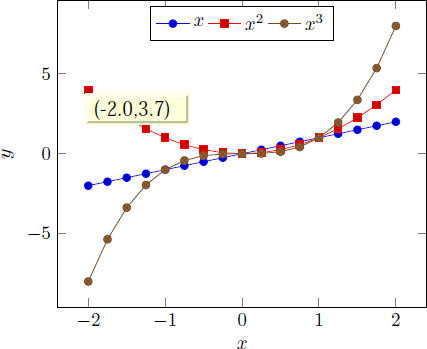
\includegraphics[height=6cm]{figures/pgfplotsclickable-fig1.png}
	\rlap{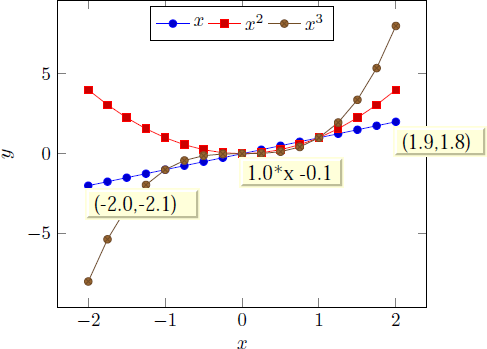
\includegraphics[height=6cm]{figures/pgfplotsclickable-fig2.png}}\hfill

	\nobreak
	These screen shots show the result of clicking into the axis range (left column) and of dragging from one point to another (right column). The second case shows the result of drag- and drop: it displays start- and end points and the equation for the line segment between between the first point of the drag- and drop and the second point where the mouse has been released. The line segment is 
	\[ l(x; x_0,y_0,x_1,y_1) = m \cdot x + n \]
	where $m = (y_1-y_0) / (x_1-x_0)$ is the slope and $n$ the offset chosen such that $l(x_0;\dotsc) = y_0$. For logarithmic plots, logarithms will be applied before computing slopes. 

	\noindent
	\hbox to \linewidth{%
	\hspace{-0.5cm}%
	\begin{tikzpicture}
		\node at (8cm,0cm)	{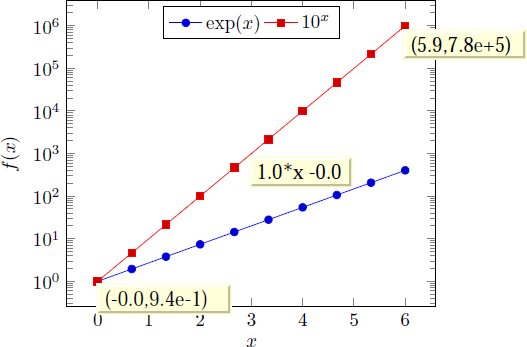
\includegraphics[height=6cm]{figures/pgfplotsclickable-fig4.png}};
		\node at (0cm,0cm)	{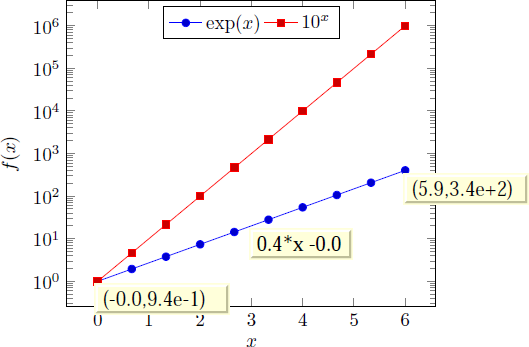
\includegraphics[height=6cm]{figures/pgfplotsclickable-fig3.png}};
	\end{tikzpicture}\hss}%

	\nobreak
	These screen shots show the result of drag- and drop for \emph{logarithmic} axes: the end points show, again, the coordinates (without logs) and the form field in the middle shows the slope and offset of the linear equation in log coordinates.

	The log basis for any logarithmic axes is usually~$10$, but it respects the current setting of |log basis x| and |log basis y|. The applied log will always use the same logarithm which is also used for the axis descriptions (this is not necessarily the same as used by \PGFPlotstable!).

	This document has been produced with the |clickable| library, so it is possible to load it into Acrobat Reader and simply click into a plot.
	
	\expandafter\ifx\csname pgfplotsclickabledisabled\endcsname\relax
	\else
	\paragraph{Attention:} For this document, the |clickable| library has been deactivated. You may find a different version on \url{http://sourceforge.net/projects/pgfplots}.
	\fi

	A click places an annotation at the coordinate under the mouse pointer, a snap--to--nearest feature is not available (yet?).

	\paragraph{Requirements:}
	\begin{itemize}
		\item The library relies on the \LaTeX\ packages |insdljs| (``Insert document level Javascript'') and |eforms| which are both part of the freely available |AcroTeX| education bundle~\cite{acrotex}\footnote{These packages rely on \LaTeX, so the library is only available for \LaTeX, not for plain \TeX\ or Con\TeX t.}. The |insdljs| package creates a temporary file with extension |.djs|.
		
		\item At the time of this writing, only Adobe Acrobat Reader interpretes Javascript and Forms properly. The library doesn't have any effect if the resulting document is used in other viewers (as far as I know).

	\end{itemize}
	Note that although this library has been written for \PGFPlots, it can be used independently of an \PGFPlots\ environment.

	\paragraph{Compatibility issues:}
	There a several restrictions when using this library. Most of them will vanish in future versions -- but up to now, I can't do magic.
	\begin{itemize}
		\item The library does not yet support rotated axes. Use |clickable=false| for those axes.
		\item The library works only with |pdflatex|, |dvips| or |dvipdfm| are not supported\footnote{In fact, they should be. I don't really know why they don't $\hdots$ any hint is welcome.}.

		\item Up to now, it is \emph{not} possible to use this library together with the |external| library and other image externalization methods of section~\ref{sec:pgfplots:importexport}.
		
		To be more precise, you can (with two extra preamble lines, see below) get correctly annotated, exported \pdf\ documents, but the |\includegraphics| command does not import the dynamic features.

		In case you decide to use this work--around, you need to insert
\begin{codeexample}[code only]
% \maxdeadcycles=10000 % in case you get the error `Output loop---<N> consecutive dead cycles.'
\usepackage[pdftex]{eforms}	
\end{codeexample}
		\noindent \emph{before} loading \pgfname, \Tikz\ or \PGFPlots. The |\maxdeadcycles| appears to be necessary for large documents, try it out.

		As long as you are working on a draft version of your document, you might want to use
\begin{codeexample}[code only]
\pgfkeys{/pgf/images/include external/.code={\href{file:#1}{\pgfimage{#1}}}
\end{codeexample}
		in your preamble. This will generate hyper links around the graphics files which link to the exported figures. Clicking on the hyper links opens the exported figure which, in turn, has been generated with the |clickable| library and allows dynamic features\footnote{This special treatment needs the external files in the same base directory as the main document, so this approach is most certainly \emph{not} suitable for a final document.}.


		\item The library automatically calls |\begin{Form}| at |\begin{document}| and |\end{Form}| at the end of the document. This environment of |hyperref| is necessary for dynamic user interaction and should be kept in mind if the document contains other form elements.
	\end{itemize}

	\paragraph{Acknowledgements:}
	\begin{itemize}
		\item I have used a javascript |sprintf| implementation of Kevin van Zonneveld~\cite{phptojs} (the javascript API has only a limited set of conversions).
	\end{itemize}
\end{pgfplotslibrary}

It is possible to customize |pgfplots.clickable| with several options.

\begin{pgfplotskey}{clickable=\mchoice{true,false} (initially true)}
	Allows to disable the library for single plots.
\end{pgfplotskey}

\begin{pgfplotskey}{annot/js fillColor=\marg{javascript color} (initially ["RGB",1,1,.855])}
	Sets the background (fill) color of the short popup annotations. 
	
	Possible choices are |transparent|, gray, RGB or CMYK color specified as four--element--arrays of the form
	|["RGB", |\meta{red}|,|\meta{green}|,|\meta{blue}|]|. Each color component is between $0$ and $1$.

	Again: this option is for Javascript. It is \emph{not} possible to use colors as in \pgfname.
\end{pgfplotskey}

\begin{pgfplotskey}{annot/point format=\marg{sprintf-format} (initially {(\%.1f,\%.1f)})}
	Allows to provide an |sprintf| format string which is used to fill the annotations with text. 
	The first argument to |sprintf| is the $x$-coordinate and the second argument is the $y$-coordinate.

	The |every semilogx axis|, |every semilogy axis| and |every loglog axis| styles have been updated to
\begin{codeexample}[code only]
\pgfplotsset{
	every semilogy axis/.append style={/pgfplots/annot/point format={(\%.1f,\%.1e)}},
	every semilogx axis/.append style={/pgfplots/annot/point format={(\%.1e,\%.1f)}},
	every loglog axis/.append style={/pgfplots/annot/point format={(\%.1e,\%.1e)}}
}
\end{codeexample}
	\noindent such that every logarithmic coordinate is displayed in scientific format.
\end{pgfplotskey}

\begin{pgfplotskey}{annot/slope format=\marg{sprintf-format} (initially \%.1f*x \%+.1f)}
	Allows to provide an |sprintf| format string which is used to fill the slope--annotation with text.
	The first argument is the slope and the second the line offset.
\end{pgfplotskey}

\begin{pgfplotskey}{annot/printable=\mchoice{true,false} (initially false)}
	Allows to configure whether the small annotations will be printed. Otherwise, they are only available on screen.
\end{pgfplotskey}

\begin{pgfplotskey}{annot/font=\marg{javascript font name} (initially font.Times)}
	Allows to choose a javascript font for the annotations. Possible choices are limited to what javascript accepts (which is \emph{not} the same as \LaTeX). The default fonts and its names are shown below.

	\begin{center}
	\begin{tabular}{ll}
		\toprule
		Font Name	& Name in Javascript\\
		\midrule
		Times-Roman           & font.Times\\
        Times-Bold            & font.TimesB\\
        Times-Italic          & font.TimesI\\
        Times-BoldItalic      & font.TimesBI\\
        Helvetica             & font.Helv\\
        Helvetica-Bold        & font.HelvB\\
        Helvetica-Oblique     & font.HelvI\\
        Helvetica-BoldOblique & font.HelvBI\\
        Courier               & font.Cour\\
        Courier-Bold          & font.CourB\\
        Courier-Oblique       & font.CourI\\
        Courier-BoldOblique   & font.CourBI\\
        Symbol                & font.Symbol\\
        ZapfDingbats          & font.ZapfD\\
		\bottomrule
	\end{tabular}
	\end{center}
\end{pgfplotskey}

\begin{pgfplotskey}{annot/textSize=\marg{Size in Point} (initially 11)}
	Sets the text size of annotations in points.
\end{pgfplotskey}

\subsubsection{Using the Clickable Library in Other Contexts}
This library provides essentially one command, |\pgfplotsclickablecreate| which creates a clickable area of predefined size, combined with javascript interaction code. It can be used independently of \PGFPlots.

\begin{command}{\pgfplotsclickablecreate\oarg{required key-value-options}}
	Creates an area which is clickable. A click produces a popup which
	contains information about the point under the cursor.
	
	The complete (!) context needs to be provided using key-value-pairs, either set before
	calling this method of inside of \oarg{required key-value-options}.
	
	This command actually creates an AcroForm which invokes javascript
	whenever it is clicked. A javascript Object is created which
	represents the context (axis limits and options). This javascript
	object is available at runtime.
	
	This method is public and it is \emph{not} restricted to \PGFPlots.
	The \PGFPlots\ hook simply initialises the required key-value-pairs.

	This method does not draw anything. It initialises only a
	clickable area and javascript code.
	
	The required key-value-pairs are documented below.
	
	\paragraph{Attention:} Complete key-value validation is \emph{not} performed here. It
	can happen that invalid options will produce javascript bugs when
	opened with Acrobat Reader. Use the javascript console to find them.
\end{command}

\noindent All options described in the following are only interesting for users who intend to use this library without \PGFPlots.

\begin{pgfplotskey}{annot/width=\marg{dimension} (initially -)}
	This required key communicates the area's width to |\pgfplotsclickablecreate|. It must be a \TeX\ dimension like |5cm|.
\end{pgfplotskey}
\begin{pgfplotskey}{annot/height=\marg{dimension} (initially -)}
	This required key communicates the area's height to |\pgfplotsclickablecreate|. It must be a \TeX\ dimension like |5cm|.
\end{pgfplotskey}
\begin{pgfplotskey}{annot/jsname=\marg{string} (initially -)}
	This required key communicates a unique identifier to |\pgfplotsclickablecreate|. This identifier is used to identify the object in javascript, so there can't be more than one of them. If it is empty, a default identifier will be created.
\end{pgfplotskey}

\begin{pgfplotskeylist}{annot/xmin=\marg{number},annot/xmax=\marg{number},annot/ymin=\marg{number},annot/ymax=\marg{number} (initially empty)}
	These required keys communicate the axis limits to |\pgfplotsclickablecreate|. They should be set to numbers which can be assigned to a javascript floating point number (standard IEEE double precision).
\end{pgfplotskeylist}

\input pgfplots.libs.units.tex
\input pgfplots.libs.groupplot.tex

\subsection{Image Externalization}
\begin{pgfplotslibrary}{external}
	The |external| library offers a convenient method to export every single |tikzpicture| into a separate~|.pdf| (or~|.eps|). Later runs of \LaTeX\ will simply include these graphics, thereby reducing typesetting time considerably.
	
	This library is documented in more detail in section~\ref{sec:pgfplots:export} ``Export to {\pdf/\eps}''.


	The |external| library has been written by Christian Feuers\"anger (author of \PGFPlots). It has been contributed to \Tikz\ as general purpose library, so the reference documentation along with all tweaks can be found in~\cite[Section ``Externalization Library'']{tikz}. The command |\usepgfplotslibrary{external}| is actually just a wrapper which loads |\usetikzlibrary{external}| or, if this library does not yet exist because the installed \pgfname\ has at most version $2.00$, it will load a copy which is shipped with \PGFPlots.
\end{pgfplotslibrary}
%
\section{Memory and Speed considerations}
\subsection{Memory Limits of \TeX}
\label{sec:pgfplots:optimization}
\PGFPlots\ can typeset plots with several thousand points if memory limits of \TeX\ are configured properly. Its runtime is roughly proportional to the number of input points\footnote{In fact, the runtime is pseudo--linear: starting with about $100{,}000$ points, it will become quadratic. This limitation applies to the path length of \PGF\ paths as well. Furthermore, the linear runtime is not possible yet for stacked plots.}.

\pgfplotsexpensiveexample
\begin{codeexample}[]
\begin{tikzpicture}
\begin{axis}[
	enlargelimits=0.01,
	title style={yshift=5pt},
	title=Scatter plot with $2250$ points]
	
\addplot[blue,
	mark=*,only marks,mark options={scale=0.3}]
	file[skip first]
	{plotdata/pgfplots_scatterdata3.dat};
	
\end{axis}
\end{tikzpicture}
\end{codeexample}

\pgfplotsexpensiveexample
\begin{codeexample}[]
\begin{tikzpicture}
\begin{axis}[
	enlarge x limits=0.03,
	title=Ornstein-Uhlenbeck sample
		($13000$ time steps),
	xlabel=$t$]
	
\addplot[blue] file {plotdata/ou.dat};
\end{axis}
\end{tikzpicture}
\end{codeexample}

\pgfplotsexpensiveexample
\begin{codeexample}[]
\begin{tikzpicture}
\begin{axis}[
	title=$120 \times 120$ Smooth Surface,
	xlabel=$x$,
	ylabel=$y$]
\addplot3[surf,samples=120,shader=interp,domain=0:1] 
	{sin(deg(8*pi*x))* exp(-20*(y-0.5)^2) 
	+ exp(-(x-0.5)^2*30 
		- (y-0.25)^2 - (x-0.5)*(y-0.25))};
\end{axis}
\end{tikzpicture}
\end{codeexample}

\PGFPlots\ relies completely on \TeX\ to do all typesetting. It uses the front-end-layer and basic layer of \PGF\ to perform all drawing operations. For complicated plots, this may take some time, and you may want to read section~\ref{sec:pgfplots:importexport} for how to write single figures to external graphics files. Externalization is the best way to reduce typesetting time.

However, for large scale plots with a lot of points, limitations of \TeX's capacities are reached easily.

\subsection{Memory Limitations}
The default settings of most \TeX-distributions are quite restrictive, so it may be necessary to adjust them. 

Usually, the log--file or the final error message contains a summary about the used resources, giving a hint which parameter needs to be increased.

\subsubsection{Mik\TeX}
For Mik\TeX, memory limits can be increased in two ways. The first is to use command line switches:
\begin{codeexample}[code only]
pdflatex 
	--stack-size=n --save-size=n 
	--main-memory=n --extra-mem-top=n --extra-mem-bot=n
	--pool-size=n --max-strings=n 
\end{codeexample}
\noindent Experiment with these settings if Mik\TeX\ runs out of memory. Usually, one doesn't invoke |pdflatex| manually: there is a development aid which does all the invocations, so this one needs to be adjusted. 

Sometimes it might be better to adjust the Mik\TeX\ configuration file permanently, for example to avoid reconfiguring the \TeX\ development program. This can be realized using the command
\begin{codeexample}[code only]
initexmf --edit-config-file=pdflatex
\end{codeexample}
\noindent which can be typed either on a command prompt in Windows or using Start $\gg$ Execute. As a result, an editor will be opened with the correct config file. A sample config file could be
\begin{codeexample}[code only]
main_memory=90000000
save_size=80000
\end{codeexample}
or any of the config file entries which are listed below can be entered. 
Thanks to ``LeSpocky'' for his documentation in

\url{http://blog.antiblau.de/2009/04/21/speicherlimits-von-miktex-erhoehen}.

\subsubsection{\TeX Live or similar installations}
For Unix installations, one needs to adjust config files. This can be done as follows:
\begin{enumerate}
	\item Locate |texmf.cnf| on your system. On my Ubuntu installation, it is in 
	
	|/usr/share/texmf/web2c/texmf.cnf|.
	\item Either change |texmf.cnf| directly, or copy it to some convenient place. If you copy it, here is how to proceed:
		\begin{itemize}
			\item keep only the changed entries in your local copy to reduce conflicts. \TeX\ will always read \emph{all} config files found in its search path.
			\item Adjust the search path to find your local copy. This can be done using the environment variable |TEXMFCNF|. Assuming your local copy is in |~/texmf/mytexcnf/texmf.cnf|, you can write
\begin{codeexample}[code only]
export TEXMFCNF=~/texmf/mytexcnf:
\end{codeexample}
			to search first in your directory, then in all other system directories.
		\end{itemize}
	\item You should change the entries
\begin{codeexample}[code only]
main_memory = n
extra_mem_top = n
extra_mem_bot = n
max_strings = n
param_size = n
save_size = n
stack_size = n
\end{codeexample}
		The log--file usually contains information about the parameter which needs to be enlarged.
\end{enumerate}
An example of this config file thing is shown below. It changes memory limits.
\begin{enumerate}
	\item Create the file |~/texmf/mytexcnf/texmf.cnf| (and possibly the paths as well).
\begin{codeexample}[code only]
% newly created file ~/texmf/mytexcnf/texmf.cnf:
% If you want to change some of these sizes only for a certain TeX
% variant, the usual dot notation works, e.g.,
% main_memory.hugetex = 20000000
main_memory = 230000000 % words of inimemory available; also applies to inimf&mp
extra_mem_top = 10000000     % extra high memory for chars, tokens, etc.
extra_mem_bot = 10000000     % extra low memory for boxes, glue, breakpoints, etc.
save_size = 150000	% for saving values outside current group
stack_size = 150000	% simultaneous input sources

% Max number of characters in all strings, including all error messages,
% help texts, font names, control sequences.  These values apply to TeX and MP.
%pool_size = 1250000
% Minimum pool space after TeX/MP's own strings; must be at least
% 25000 less than pool_size, but doesn't need to be nearly that large.
%string_vacancies = 90000
% Maximum number of strings.
%max_strings = 100000
% min pool space left after loading .fmt
%pool_free = 47500
\end{codeexample}
	\item Run |texhash| such that \TeX\ updates its |~/texmf/ls-R| database.
	\item Create the environment variable |TEXMFCNF| and assign the value `|~/texmf/mytexcnf:|' (including the trailing `|:|'!). For my linux system, this can be done using by adding
\begin{codeexample}[code only]
export TEXMFCNF=~/texmf/mytexcnf:
\end{codeexample}
	to |~/.bashrc|.
\end{enumerate}

Unfortunately, \TeX\ does not allow arbitrary memory limits, there is an upper bound hard coded in the executables.

\subsection{Reducing Typesetting Time}
\PGFPlots\ does a lot of computations ranging from abstract coordinate computations to low level |.pdf| drawing commands (realized by \PGF). For complex plots, this may take a considerable time -- especially for 3D plots.

One possibility to reduce typesetting time is to tell \PGF\ to generate single, temporary |.pdf| (or |.eps|) documents for a subset (or all) graphics in one run and re-use these temporary images in successive runs. For \PGFPlots, this is the most effective way to reduce typesetting time. It can be accomplished using the |external| library described in section~\ref{sec:pgfplots:export}.
%
\section{Import/Export From Other Formats}
\label{sec:pgfplots:importexport}
This section contains information of how to single pictures into separate \pdf\ graphics files (or \eps\ graphics files). Furthermore, it explains a matlab (tm) script which allows to convert from matlab to \PGFPlots.

\subsection[Export to pdf/eps]{Export to {\normalfont\pdf/\eps}}
\label{sec:pgfplots:export}
It is possible to export images to single \pdf-documents using routines of \pgfname\ and/or \Tikz.

\subsubsection{Using the Automatic Externalization Framework of \Tikz}
\begin{pgfplotslibrary}{external}
\pgfkeys{
	/pdflinks/search key prefixes in/.add={/tikz/external/,}{}
}
	The |external| library offers a convenient method to export every single |tikzpicture| into a separate~|.pdf| (or~|.eps|). Later runs of \LaTeX\ will simply include these graphics, thereby reducing typesetting time considerably.

	The library can also be used to submit documents to authors who do not even have \PGFPlots\ or \Tikz\ installed.

	\paragraph{Technical foreword:}
	The |external| library has been written by Christian Feuers\"anger (author of \PGFPlots). It has been contributed to \Tikz\ as general purpose library, so the reference documentation along with all tweaks can be found in~\cite[Section ``Externalization Library'']{tikz}. The command |\usepgfplotslibrary{external}| is actually just a wrapper which loads |\usetikzlibrary{external}| or, if this library does not yet exist because the installed \pgfname\ has at most version $2.00$, it will load a copy which is shipped with \PGFPlots.

	The |external| library has been designed such that \emph{no changes} to the document as such are necessary. The idea is as follows:
\begin{enumerate}
	\item Every |\begin{tikzpicture}| $\dotsc$ |\end{tikzpicture}| gets a file name. The file name can be assigned manually with |\tikzsetnextfilename|\marg{output file name} or automatically, in which case \meta{tex file name}|-figure|\meta{number} is used with an increasing \meta{number}.
	
	\item The library writes the resulting images using system calls of the form |pdflatex --jobname |\marg{output file name} automatically, using the write18 system call of \TeX. It is the same framework which can be used to call |gnuplot|.
\end{enumerate}
The only steps which are necessary is to use

\pgfmanualpdflabel{\textbackslash tikzexternalize}{}%
|\usepgfplotslibrary{external}|

|\tikzexternalize|

\noindent somewhere in your document's preamble. No further modification to the document is necessary. Suppose we have a file called |test.tex|:
\begin{codeexample}[code only]
\documentclass{article}

\usepackage{pgfplots}

\usepgfplotslibrary{external}
\tikzexternalize% activate externalization!

\begin{document}
	\begin{figure}
		\begin{tikzpicture}
		\begin{axis}
			\addplot {x^2};
		\end{axis}
		\end{tikzpicture}
	\caption{Our first external graphics example}
	\end{figure}

	\begin{figure}
		\begin{tikzpicture}
		\begin{axis}
			\addplot {x^3};
		\end{axis}
		\end{tikzpicture}
	\caption{A second graphics}
	\end{figure}
\end{document}
\end{codeexample}
\noindent To enable the system calls, we type
\begin{codeexample}[code only]
pdflatex -shell-escape test
\end{codeexample}
\noindent and \LaTeX\ will now generate the required graphics files |test-figure0.pdf| and |test-figure1.pdf| automatically. Any further call to |pdflatex| will simply use |\includegraphics| and the |tikzpicture|s as such are no longer considered (you need a different command line switch for Mik\TeX, see the |shell escape| option).

If a figure shall be remade, one can simply delete all or selected graphics files and re-generate them. Alternatively, one can use the command |\tikzset{external/force remake}| somewhere in the document to remake every following picture automatically.

There are three ways to modify the file names of externalized figures:
\begin{itemize}
	\item Changing the overall file name using a |prefix|,
	\item Changing the file name for a single figure using |\tikzsetnextfilename|,
	\item Changing the file name for a restricted set of figures using |figure name|.
\end{itemize}
\begin{key}{/tikz/external/prefix=\marg{file name prefix} (initially empty)}
	A shortcut for |\tikzsetexternalprefix|\marg{file name prefix}, see below.
\end{key}

\begin{command}{\tikzsetexternalprefix\marg{file name prefix}}
	Assigns a common prefix used by all file names. For example,
\begin{codeexample}[code only]
\tikzsetexternalprefix{figures/}
\end{codeexample}
	will prepend |figures/| to every external graphics file name.
\end{command}

\begin{command}{\tikzsetnextfilename\marg{file name}}
	Sets the file name for the \emph{next} \tikzname\ picture or |\tikz| short command. It will \emph{only} be used for the next picture.

	Pictures for which no explicit file name has been set will get automatically generated file names.

	Please note that |prefix| will still be prepended to \marg{file name}.
\begin{codeexample}[code only]
\documentclass{article}
% main document, called main.tex
\usepackage{tikz}

\usepgfplotslibrary{external}
\tikzexternalize[prefix=figures/]% activate with a name prefix

\begin{document}

\tikzsetnextfilename{firstplot}
\begin{tikzpicture} % will be written to 'figures/firstplot.pdf'
\begin{axis}
	\addplot {x};  	
\end{axis}
\end{tikzpicture}

\begin{tikzpicture} % will be written to 'figures/main-figure0.pdf'
   \draw[help lines] (0,0) grid (5,5);
\end{tikzpicture}
\end{document}
\end{codeexample}
\begin{codeexample}[code only]
pdflatex -shell-escape main
\end{codeexample}
\end{command}

\begin{key}{/tikz/external/figure name=\marg{name}}
	Same as |\tikzsetfigurename|\marg{name}.
\end{key}
\begin{command}{\tikzsetfigurename\marg{name}}
	Changes the names of \emph{all} following figures. It is possible to change |figure name| during the document using |\tikzset{external/figure name|=\marg{name}|}|. A unique counter\footnote{These counters are stored into into different \emph{macros}. In other words: no \TeX\ register will be needed.} will be used for each different \marg{name}, and each counter will start at $0$.

	The value of |prefix| will be applied after |figure name| has been evaluated.
\begin{codeexample}[code only]
\documentclass{article}
% main document, called main.tex
\usepackage{tikz}

\usepgfplotslibrary{external}
\tikzexternalize% activate externalization!

\begin{document}

% will be written to 'main-figure0.pdf'
\begin{tikzpicture} 
\begin{semilogyaxis}
	\addplot {exp(x)};
\end{semilogyaxis}
\end{tikzpicture}

{
  \tikzset{external/figure name={subset_}}
  A simple image is \tikz \fill (0,0) circle(5pt);. % will be written to 'subset_0.pdf'

  \begin{tikzpicture} % will be written to 'subset_1.pdf'
     \begin{axis}
	 	\addplot {x^2};
	\end{axis}
  \end{tikzpicture}
}% here, the old file name will be restored:

\begin{tikzpicture} % will be written to 'main-figure1.pdf'
   \begin{axis}
   		\addplot[domain=1e-3:100] {1/x};
	\end{axis}
\end{tikzpicture}
\end{document}
\end{codeexample}
	The scope of |figure name| ends with the next closing brace (as all values set by |\tikzset| do).

	\medbreak
	Remark: Use |\tikzset{external/figure name/.add=|\marg{prefix}\marg{suffix}|}| to prepend  a \meta{prefix} and append a \meta{suffix} to the actual value of |figure name|. Might be useful for something like
\begin{codeexample}[code only]
\tikzset{external/figure name=main}

% uses main_0.pdf, main_1.pdf, ...

\section{The first section}
{\tikzset{external/figure name/.add={}{_firstsection}}
	...
	% uses main_firstsection_0.pdf, main_firstsection_1.pdf, ...
}

\section{The second section}
{\tikzset{external/figure name/.add={}{secondsection_}}
	...
	% uses main_secondsection_0.pdf, main_secondsection_1.pdf, ...
	\subsection{Second subsection}
	{\tikzset{external/figure name/.add={}{sub_}}
		...
		% uses main_secondsection_sub_0.pdf, main_secondsection_sub_1.pdf, ...
	}
	% uses main_secondsection_2.pdf, main_secondsection_3.pdf, ...
}
\end{codeexample}
\end{command}

\begin{command}{\tikzappendtofigurename\marg{suffix}}
	Appends \meta{suffix} to the actual value of |figure name|.

	It is a shortcut for |\tikzset{external/figure name/.add={}|\marg{suffix}|}| (a shortcut which is also supported if \tikzname\ is not installed, see below).
\end{command}


\begin{key}{/tikz/external/system call=\marg{template}}
\label{extlib:systemcall:option}
	A template string used to generate system calls. Inside of \marg{template}, the macro |\image| can be used as placeholder for the image which is about to be generated while |\texsource| contains the main file name (in truth, it contains |\input|\marg{main file name}, but that doesn't matter).

	The default is 
\begin{codeexample}[code only]
\tikzset{external/system call={pdflatex \tikzexternalcheckshellescape -halt-on-error 
    -interaction=batchmode -jobname "\image" "\texsource"}
\end{codeexample}
	\noindent where \declareandlabel{\tikzexternalcheckshellescape} inserts the value of the configuration key |shell escape|
	if and only if the current document has been typeset with |-shell-escape|\footnote{Note that this is always true for the default configuration. This security consideration applies mainly for \texttt{mode=list and make} which will also work \emph{without} shell escapes.}.

	For |eps| output, you can (and need to) use
\begin{codeexample}[code only]
\tikzset{external/system call={latex \tikzexternalcheckshellescape -halt-on-error
    -interaction=batchmode -jobname "\image" "\texsource"; 
    dvips -o "\image".ps "\image".dvi}}
\end{codeexample}
	
	The argument \marg{template} will be expanded using |\edef|, so any control sequences will be expanded. During this evaluation, `|\\|' will result in a normal backslash, `|\|'. Furthermore, double quotes `|"|', single quotes `|'|', semicolons and dashes `|-|' will be made to normal characters if any package uses them as macros. This ensures compatibility with the |german| package, for example.
\end{key}

\begin{key}{/tikz/external/shell escape=\marg{command-line arg} (initially -shell-escape)}
	Contains the command line option for |latex| which enables the |\write18| feature. For \TeX-Live, this is |-shell-escape|. For Mik\TeX, you should use |\tikzexternalize[shell escape=-enable-write18]|.
\end{key}

\paragraph{Support for Labels and References In External Files}
The |external| library comes with extra support for |\label| and |\ref| (and other commands which usually store information in the |.aux| file) inside of external files.

There are, however, some points which need your attention when you try to use 
\begin{enumerate}
	\item[a)] |\ref| to something in the main document inside of an externalized graphics or
	\item[b)] |\label| in the externalized graphics which is referenced in the main document.
\end{enumerate}

For point a), a |\ref| inside of an externalized graphics works \emph{only} if you issue the required system call \emph{manually} or by |make|. The initial configuration |mode=convert with system call| does \emph{not} support |\ref|. But you can copy--paste the system call generated by |mode=convert with system call| and issue it manually. The reason is that |\ref| information is stored in the main |.aux| file -- but this auxiliary file is not completely written when |mode=convert with system call| is invoked (there is a race condition). Note that |\pageref| is not supported (sorry). Thus: if you have |\ref| inside of external graphics, consider using |mode=list and make| or copy--paste the system call for the image(s) and issue it manually.

Point b) is realized automatically by the external library. In detail, a |\label| inside of an externalized graphics causes the external library to generate separate auxiliary files for every external image. These files are called \meta{imagename}|.dpth|. The extension |.dpth| indicates that the file also contains the image's depth (the |baseline| key of \tikzname). Furthermore, anything which would have been written to an |.aux| file will be redirected to the |.dpth| file -- but only things which occur inside of the externalized |tikzpicture| environment. When the main document loads the image, it will copy the |.dpth| file into the main |.aux| file. Then, successive compilations of the main document contain the external |\label| information. In other words, a |\label| in an external graphics needs the following work flow:
\begin{enumerate}
	\item The external graphics needs to be generated together with its |.dpth| (usually automatically by \tikzname).
	\item The main document includes the external graphics and copies the |.dpth| content into its main |.aux| file.
	\item The main document needs to be translated one further time to re-read its |.aux| file\footnote{Note that it is not possible to activate the content of an auxiliary file after \texttt{\textbackslash begin\{document\}} in \LaTeX.}.
\end{enumerate}
There is just one special case which occurs if a |\label|/|\ref| combination is realized itsself by a |tikzpicture|. This is, for example, the case for the legend |\ref| images or for the |\pgfplotslegendfromname| feature. In such cases, you need to proceed as for case a) since |mode=convert with system call| can't handle that stuff on its own. 

In other words: a |\label| in an external document works automatically, just translate the main document often enough. A |\ref| might need manual adjustments as described for case a) above.


\paragraph{Operation Modes}
\begin{key}{/tikz/external/mode=\mchoice{convert with system call,list and make,$\dotsc$} (initially convert with system call)}
	This allows to change the default operation mode. There are a handful of choices possible, all of them are described in detail in~\cite[section ``Externalization Library'']{tikz}. The most useful ones are probably the initial configuration |convert with system call| and the specialized choice |list and make|.
	
	The choice |list and make| configures the library to check if there are already external graphics and uses them. If there are no graphics, the library will \emph{skip} the figure. However, it will also generate a |makefile| to generate the graphics, and a list of all required graphics files.

	It is not required to use |make|: the library expects you to generate the images somehow and it doesn't care about the ``how''. Using |make -f |\meta{name-of-tex-file}|.makefile -j 2| allows parallel execution which might, indeed, be an option. Furthermore, the makefile also supports file dependencies: if one of your data tables has been updated, the external graphics will be remade automatically. \PGFPlots\ tells the external library about any file dependencies (input files and tables).

	The two modes have the following characteristics:
	\begin{enumerate}
		\item |convert with system call| is automatic and does everything on--the--fly. However, it \emph{can't} work with |\ref| and/or |\label| information in external pictures.
		\item |list and make| requires either manual (by calling the system calls manually) or semi--automatic conversion (using the generated \meta{main}|.makefile|), and multiple runs of |pdflatex|. The generated Makefile can be processed in parallel. Furthermore, |list and make| provides \emph{full support} for |\ref| and |\label|: any |\label| defined inside of an externalized graphics is still available for the main document.
		
		If you have legends with |legend to name| or |\label|/|\ref|, you need to generate the graphics defining the |\label| (or |legend to name|), then run |pdflatex| twice on the main document. Afterwards, you can externalize the legend graphics.
	\end{enumerate}
\end{key}

The complete reference documentation and remaining options are documented in~\cite[``Externalization Library'']{tikz}. This reference also contains information about
\begin{itemize}
	\item how to use |\tikzset{external/|\declareandlabel{force remake}|}| and |\tikzset{external/|\declareandlabel{remake next}|}| to remake selected figures,
	\item how to disable the externalization partially with |\tikzset{external/|\declareandlabel{export}|=false}| or completely with |\tikzexternaldisable|,
	\item how to optimize the speed of the conversion process using |\tikzset{external/optimize command away=\myExpensiveMacro}|,
	\item how to add further remake-dependencies with |\tikzpicturedependsonfile|\marg{name} and/or  |\tikzexternalfiledependsonfile|\marg{external file}\marg{name},
	\item how to typeset such a document without \pgfname\ installed or
	\item how to provide work-arounds with |.pdf| images and bounding box restrictions.
\index{External Graphics!Bounding Box Issues}
\index{Bounding Box Control!Image Externalization Problems}
\end{itemize}

\paragraph{Using the Library Without {\normalfont\pgfname} or {\normalfont\PGFPlots} Installed}
There is a small replacement package \declareandlabel{tikzexternal.sty} which can be used once every figure has been exported. The idea is to uncomment |\usepackage{tikz}| and |\usepackage{pgfplots}| and write |\usepackage{tikzexternal}| instead:
\begin{codeexample}[code only]
% \usepackage{tikz}
% \usepackage{pgfplots}
\usepackage{tikzexternal}
\tikzexternalize% activate externalization

\begin{document}
\begin{tikzpicture}
	...
\end{tikzpicture}
...
\end{document}
\end{codeexample}
You do not need \pgfname, \tikzname\ or \PGFPlots\ installed. What you need is |tikzexternal.sty| and all generated figures (consisting of the image files, `|.pdf|' and the `|.dpth|' files containing information of the |baseline| option). The file |tikzexternal.sty| is shipped with \pgfname\ in the directory
\begin{codeexample}[code only]
latex/pgf/utilities/tikzexternal.sty
\end{codeexample}
and a copy is shipped with \PGFPlots\ in
\begin{codeexample}[code only]
tex/generic/pgfplots/oldpgfcompatib/pgfplotsoldpgfsupp_tikzexternal.sty
\end{codeexample}
Just copy the file into your directory and rename it to |tikzexternal.sty|.

\paragraph{Attention:} The small replacement package doesn't support key--value interfaces. Thus, it is necessary to use |\tikzsetexternalprefix| instead of the |prefix| option and |\tikzsetfigurename| instead of the |figure name| option since |\tikzset| is not available in such a context. Also, you may want to define a dummy--macro |\pgfplotsset| if you have used |\pgfplotsset|.
\end{pgfplotslibrary}

\subsubsection[Using the Externalization Framework of PGF By Hand]{Using the Externalization Framework of {\normalfont\pgfname} ``By Hand''}
Another way to export \TeX-pictures to single graphics files is to use the externalization framework of \pgfname, which requires more work but works more generally than the |external| library.
The basic idea is to encapsulate the desired parts with

\declareandlabel{\beginpgfgraphicnamed}\marg{output file name}

\meta{picture contents}

\declareandlabel{\endpgfgraphicnamed}. 

\noindent Furthermore, one needs to tell \pgfname\ the name of the main document using

\declareandlabel{\pgfrealjobname}\marg{the real job's name}

\noindent in the preamble. This enables two different modes: 
\begin{enumerate}
	\item The first is the normal typesetting mode. \LaTeX\ checks whether a file named \marg{output file name} with one of the accepted file extensions exists -- if that is the case, the graphics file is included with |\pgfimage| and the \meta{picture contents} is skipped. If no such file exists, the \meta{picture contents} is typeset normally. This mode is applied if |\jobname| equals \marg{the real job's name}.
	\item The second mode applies if |\jobname| equals \marg{output file name}, it initiates the ``conversion mode'' which is used to write the graphics file \marg{output file name}. In this case, \emph{only} \meta{picture contents} is written to |\jobname|, the complete rest of the \LaTeX\ is processed as normal, but it is silently discarded.

	This mode needs to be started manually with |pdflatex --jobname |\meta{output file name} for every externalized graphics file.
\end{enumerate}
A complete example may look as follows.
\begin{codeexample}[code only]
\documentclass{article}

\usepackage{pgfplots}

\pgfrealjobname{test}

\begin{document}
	\begin{figure}
		\beginpgfgraphicnamed{testfigure}
		\begin{tikzpicture}
		\begin{axis}
			\addplot {x^2};
		\end{axis}
		\end{tikzpicture}
		\endpgfgraphicnamed
	\caption{Our first external graphics example}
	\end{figure}

	\begin{figure}
		\beginpgfgraphicnamed{testfigure2}
		\begin{tikzpicture}
		\begin{axis}
			\addplot {x^3};
		\end{axis}
		\end{tikzpicture}
		\endpgfgraphicnamed
	\caption{A second graphics}
	\end{figure}
\end{document}
\end{codeexample}
\noindent The file is named |test.tex|, and it is processed (for example) with
\begin{codeexample}[code only]
pdflatex test	
\end{codeexample}
\noindent Now, we type
\begin{codeexample}[code only]
pdflatex --jobname testfigure test	
pdflatex --jobname testfigure2 test	
\end{codeexample}
\noindent to enter conversion mode. These last calls will \emph{only} write the contents of our named graphics environments, one for \marg{testfigure} and one for \marg{testfigure2} into the respective output files |testfigure.pdf| and |testfigure2.pdf|.

In summary, one needs |\pgfrealjobname| and calls |pdflatex --jobname |\marg{graphics file} for every externalized graphics environment. Please note that it is absolutely necessary to use the syntax above, \emph{not} |\begin{pgfgraphicnamed}|.

These steps are explained in much more detail in Section``Externalizing Graphics'' of~\cite{tikz}.

\paragraph{Attention:} Do not forget a correct |\pgfrealjobname| statement! If it is missing, externalization simply won't work. If it is wrong, any call to \LaTeX\ will produce empty output files.

It should be noted that this approach of image externalization is not limited to \Tikz\ picture environments. In fact, it collects everything between the begin and end statements into the external file. It is implicitly assumed that the encapsulated stuff is one box, but you can also encapsulate complete paragraphs using something like the \LaTeX\ minipage (or a |\vbox| which is not as powerful but does not affect the remaining document that much).

\begin{key}{/pgf/images/aux in dpth=\mchoice{true,false} (initially false)}
	If this boolean is set to |true|, any |\label| information generated inside of the external image is stored into the already mentioned |.dpth| file. The main document can thus reference label information of externalized parts of the document (although you may need to run |latex| several times). 

	Label support is provided for |\ref|, and probably |\cite|. The |\pageref| command is only partially supported.
\end{key}

\paragraph{Using the Library Without {\normalfont\pgfname} Installed}
Simply uncomment the packages |\usepackage{tikz}| and |\usepackage{pgfplots}| and use
\begin{codeexample}[code only]
\long\def\beginpgfgraphicnamed#1#2\endpgfgraphicnamed{%
	\begingroup
	\setbox1=\hbox{\includegraphics{#1}}%
	\openin1=#1.dpth
	\ifeof1 \box1 
	\else
		\read1 to\pgfincludeexternalgraphicsdp \closein1
		\dimen0=\pgfincludeexternalgraphicsdp\relax
		\hbox{\lower\dimen0 \box1 }%
	\fi
	\endgroup
}
\end{codeexample}
instead. This will include the generated graphics files (and it will respect the |baseline| information stored in |.dpth| files). Consequently, you won't need \pgfname\ or \PGFPlots\ installed. See Section``Externalizing Graphics'' of~\cite{tikz} for details.


\subsection{Exporting Mesh Data From Matlab To \PGFPlots}
While it is easy to write Matlab vectors to files (using |save P.dat data -ASCII|), it is more involved to export mesh data.

The main problem is to communicate the mesh structure to \PGFPlots.

Here is an example how to realize this task: in Matlab, we have mesh data |X|, |Y| and |Z| which are matrizes of the same size. For example, suppose we have

\begin{codeexample}[code only]
[X,Y] = meshgrid( linspace(-1,1,5), linspace(4,5,10) );
Z = X + Y;
surf(X,Y,Z)
\end{codeexample}
\noindent as data. Then, we can generate an $N \times 3$ table containing all single elements in column--wise ordering with

\begin{codeexample}[code only]
data = [ X(:) Y(:) Z(:) ]
save P.dat data -ASCII
\end{codeexample}
\noindent where the second command stores the $N \times 3$ table into |P.dat|. Finally, we can use 

|\addplot3[surf,mesh/rows=10,mesh/ordering=colwise,shader=interp] file {P.dat};|

in \PGFPlots\ to read this data. We need to provide either the number of rows ($10$ here) or the number of columns -- and the ordering (which is |colwise| for Matlab matrizes).

An alternative which is faster in \PGFPlots\ would be to transpose the matrizes in Matlab and tell \PGFPlots\ they are in |rowwise| ordering. So, the last step becomes

\begin{codeexample}[code only]
XX=X'; YY=Y'; ZZ=Z';
data = [ XX(:) YY(:) ZZ(:) ]
save P.dat data -ASCII
\end{codeexample}
\noindent with \PGFPlots\ command

|\addplot3[surf,mesh/cols=10,mesh/ordering=rowwise,shader=interp] file {P.dat};|.

\subsection{matlab2pgfplots.m}
This is a Matlab (tm) script which attempts to convert a matlab figure to \PGFPlots. It requires Matlab version 7.4 (or higher).

\paragraph{Attention:} The author of \PGFPlots\ does not have enough time to maintain this script as much as he wants to. In other words, it supports only a small subset of \PGFPlots. You may also want to look at |matlab2tikz|, a conversion script of Nico Schl\"omer available at

\url{http://www.mathworks.com/matlabcentral/fileexchange/22022-matlab2tikz}

\noindent which also uses \PGFPlots\ for the \LaTeX\ conversion.

\medskip
The idea of |matlab2pgfplots.m| is to
\begin{itemize}
	\item use a complete matlab figure as input,
	\item acquire axis labels, axis scaling (log or normal) and legend entries,
	\item acquire all plot coordinates
\end{itemize}
and write an equivalent \texttt{.pgf} file which typesets the plot with \PGFPlots.

The intention is \emph{not} to simulate matlab. It is a first step for a conversion. Type
\begin{lstlisting}
> help matlab2pgfplots
\end{lstlisting}
on your matlab prompt for more information about its features and its limitations.

This script is experimental.

\subsection{matlab2pgfplots.sh}
A \texttt{bash}-script which simply starts matlab and runs 
\begin{lstlisting}
	f=hgload( 'somefigure.fig' );
	matlab2pgfplots( 'outputfile.pgf', 'fig', f );
\end{lstlisting}
See matlab2pgfplots.m above.

\subsection{SVG Output}
It is possible to write every single \Tikz\ picture into a scalable vector graphics (\texttt{.svg}) file. This has nothing to do with \PGFPlots, it is a separate driver of \PGF. Please refer to~\cite[Section ``Producing HTML / SVG Output'']{tikz}.

\subsection{Generate \PGFPlots\ Graphics Within Python}
Mario Orne D\'IAZ ANAD\'ON contributed a small python script |pgfplots.py| which provides a simple interface to generate \PGFPlots\ figures from within python. It can be found in the \PGFPlots\ installation directory, in |pgfplots/scripts/pgfplots/pgfplots.py|; documentation can be found in the file.
%
\section{Utilities and Basic Level Commands}
\label{sec:pgfplots:lowlevel}
This section documents commands which provide access to more basic elements of \PGFPlots. Most of them are closely related to the basic level of \pgfname, especially various point commands which are specific to an axis. Some of them are general purpose utilities like loops.

However, most elements in this section are only interesting for advanced users -- and perhaps only for special cases.

\subsection{Utility Commands}

\begin{command}{\foreach \meta{variables} |in| \meta{list} \marg{commands}}
	A powerful loop command provided by \Tikz, see~\cite[Section Utilities]{tikz}.
\begin{codeexample}[]
\foreach \x in {1,2,...,4} {Iterating \x. }%
\end{codeexample}

	A \PGFPlots\ related example could be
\begin{codeexample}[code only]
\foreach \i in {1,2,...,10} {\addplot table {datafile\i}; }%
\end{codeexample}
\end{command}

\begin{command}{\pgfplotsforeachungrouped \meta{variable} |in| \meta{list} \marg{command}}
	A specialised variant of |\foreach| which can do two things: it does not introduce extra groups while executing \meta{command} and it allows to invoke the math parser for (simple!) \meta{$x_0$}|,|\meta{$x_1$}|,...,|\meta{$x_n$} expressions.

\begin{codeexample}[]
\def\allcollected{}
\pgfplotsforeachungrouped \x in {1,2,...,4} {Iterating \x. \edef\allcollected{\allcollected, \x}}%
All collected = \allcollected.
\end{codeexample}

	A more useful example might be to work with tables. The following example is taken from \PGFPlotstable:

\begin{codeexample}[code only]
\pgfplotsforeachungrouped \i in {1,2,...,10} {%
	\pgfplotstablevertcat{\output}{datafile\i} % appends `datafile\i' -> `\output'
}%
% since it was ungrouped, \output is still defined (would not work
% with \foreach)
\end{codeexample}

	\paragraph{Remark: } The special syntax \meta{list}=\meta{$x_0$}|,|\meta{$x_1$}|,...,|\meta{$x_n$}, i.e.\ with two leading elements, followed by dots and a final element, invokes the math parser for the loop. Thus, it allows larger number ranges than any other syntax if |/pgf/fpu| is active.  In all other cases, |\pgfplotsforeachungrouped| invokes |\foreach| and provides the results without \TeX\ groups.
	
\end{command}

\begin{command}{\pgfplotsinvokeforeach\marg{list} \marg{command}}
	A variant of |\pgfplotsforeachungrouped| (and such also of |\foreach|) which replaces any occurrence of |#1| inside of \meta{command} once for every element in \meta{list}. Thus, it actually assumes that \marg{command} is like a |\newcommand| body.

	In other words, \marg{command} is invoked for every element of \marg{list}. The actual element of \marg{list} is available as |#1|.

	As |\pgfplotsforeachungrouped|, this command does \emph{not} introduce extra scopes (i.e.\ it is ungrouped as well).

	The difference to |\foreach \x in |\meta{list}\marg{command} is subtle: the |\x| would \emph{not} be expanded whereas |#1| is. 
\begin{codeexample}[]
\pgfkeys{
  otherstyle a/.code={[a]},
  otherstyle b/.code={[b]},
  otherstyle c/.code={[c]},
  otherstyle d/.code={[d]}}
\pgfplotsinvokeforeach{a,b,c,d}        	
	{\pgfkeys{key #1/.style={otherstyle #1}}}
Invoke them: 
\pgfkeys{key a} \pgfkeys{key b} 
\pgfkeys{key c} \pgfkeys{key d}
\end{codeexample}
The counter example would use a macro (here |\x|) as loop argument:
\begin{codeexample}[]
\pgfkeys{
  otherstyle a/.code={[a]},
  otherstyle b/.code={[b]},
  otherstyle c/.code={[c]},
  otherstyle d/.code={[d]}}
\pgfplotsforeachungrouped \x in {a,b,c,d}        	
	{\pgfkeys{key \x/.style={otherstyle \x}}}
Invoke them: 
\pgfkeys{key a} \pgfkeys{key b}
\pgfkeys{key c} \pgfkeys{key d}
\end{codeexample}

	\paragraph{Restrictions:} you can't nest this command yet (since it does not introduce protection by scopes).
\end{command}

\begin{command}{\pgfmathparse\marg{expression}}
	Invokes the \pgfname\ math parser for \meta{expression} and defines \declareandlabel{\pgfmathresult} to be the result.
\begin{codeexample}[]
\pgfmathparse{1+41}

The result is `\pgfmathresult'.
\end{codeexample}
	Please refer to \cite{tikz} for more details.
\end{command}


\begin{command}{\pgfplotstableread\marg{file}}
	Please refer to the manual of \PGFPlotstable, |pgfplotstable.pdf|, which is part of the \PGFPlots-bundle.
\end{command}
\begin{command}{\pgfplotstabletypeset\marg{\textbackslash macro}}
	Please refer to the manual of \PGFPlotstable, |pgfplotstable.pdf|, which is part of the \PGFPlots-bundle.
\end{command}

\begin{command}{\pgfplotsiffileexists\marg{filename}\marg{true code}\marg{false code}}
	Invokes \marg{true code} if \marg{filename} exists and \marg{false code} if not. Can be used in looping macros, for example to plot every data file until there are no more of them.
\end{command}
\begin{command}{\pgfplotsutilifstringequal\marg{first}\marg{second}\marg{true code}\marg{false code}}
	A simple ``strcmp'' tool which invokes \marg{true code} if \marg{first} $=$\marg{second} and \marg{false code} otherwise. This does not expand macros.
\end{command}


\begin{commandlist}{\pgfkeys,\pgfeov,\pgfkeysvalueof,\pgfkeysgetvalue}
	These commands are part of the \Tikz\ way of specifying options, its sub-package |pgfkeys|. The |\pgfplotsset| command is actually nothing but a wrapper around |\pgfkeys|.

	A short introduction into |\pgfkeys| can be found in~\cite{keyvalintro} whereas the complete reference is, of course, the \Tikz\ manual~\cite{tikz}.

	The key |\pgfkeysvalueof|\marg{key name} expands to the value of a key; |\pgfkeysgetvalue|\marg{key name}\marg{\textbackslash macro} stores the value of \meta{key name} into \meta{\textbackslash macro}. The |\pgfeov| macro is used to delimit arguments for code keys in |\pgfkeys|, please refer to the references mentioned above.
\end{commandlist}

\subsection[Commands Inside Of PGFPlots Axes]{Commands Inside Of {\normalfont\PGFPlots} Axes}
\begin{command}{\autoplotspeclist}
This command should no longer be used, although it will be kept as technical implementation detail. Please use the `|cycle list|' option, section~\ref{sec:cycle:list}.
\end{command}

\begin{command}{\logten}
Expands to the constant $\log(10)$. Useful for logplots because $\log(10^i) = i\log(10)$. This command is only available inside of an \Tikz-picture.
\end{command}

\begin{command}{\pgfmathprintnumber\marg{number}}
Generates pretty--printed output\footnote{This method was previously \texttt{\textbackslash prettyprintnumber}. It's functionality has been included into \PGF\ and the old command is now deprecated.} for \marg{number}. This method is used for every tick label.

The number is printed using the current number printing options, see the manual of \PGFPlotstable\ which comes with this package for the different number styles, rounding precision and rounding methods.
\end{command}

\begin{command}{\numplots}
	Inside of any of the axis environments, associated style, option or command, |\numplots| expands to the total number of  plots.
\end{command}
\begin{command}{\numplotsofactualtype}
	Like |\numplots|, this macro returns the total number of plots which have the same plot handler. Thus, if you have |sharp plot| active, it returns the number of all |sharp plots|. If you have |ybar| active, it returns the number of |ybar| plots and so on.
\end{command}

\begin{command}{\plotnum}
	Inside of |\addplot| or any associated style, option or command, |\plotnum| expands to the current plot's number, starting with~$0$.
\end{command}

\begin{command}{\plotnumofactualtype}
	Like |\plotnum|, but it returns the number among all plots of the same type (see |\numplotsofactualtype|).	
\end{command}

\begin{command}{\coordindex}
	Inside of an |\addplot| command, this macro expands to the number of the actual coordinate (starting with~$0$).

	It is useful together with |x filter| or |y filter| to (de-)select coordinates.
\end{command}

\subsection{Path Operations}

\begin{commandlist}{\path,\draw,\fill,\node,\matrix}
	These commands are \Tikz\ drawing commands all of which are documented in~\cite{tikz}. They are used to draw or fill paths, generate text nodes or aligned text matrices. They are equivalent to 
	\pgfmanualpdflabel{/tikz/draw}{}|\path[draw]|, 
	\pgfmanualpdflabel{/tikz/fill}{}|\path[fill]|, 
	\pgfmanualpdflabel{/tikz/node}{}|\path[node]|, 
	\pgfmanualpdflabel{/tikz/matrix}{}|\path[matrix]|, 
	respectively.
\end{commandlist}
\begin{pathoperation}{--}{\meta{coordinate}}
	A \Tikz\ path operation which connects the current point (the last one before |--|) and \meta{coordinate} with a straight line.
\end{pathoperation}
{\catcode`\|=12
\begin{pathoperation}[noindex]{|-}{\meta{coordinate}}
\pgfmanualpdflabel[\catcode`\|=12 ]{|-}{}%
	A \Tikz\ path operation which connects the current point and \meta{coordinate} with \emph{two} straight lines: first vertical, then horizontal.
\end{pathoperation}

\begin{pathoperation}[noindex]{-|}{\meta{coordinate}}
\pgfmanualpdflabel[\catcode`\|=12 ]{-|}{}%
	A \Tikz\ path operation which connects the current point and \meta{coordinate} with \emph{two} straight lines: first horizontal, then vertical.
\end{pathoperation}
}

\begin{keylist}{/tikz/xshift=\marg{dimension},/tikz/yshift=\marg{dimension}}
	These \Tikz\ keys allow to shift something by \marg{dimension} which is any \TeX\ size (or expression).
\end{keylist}


\begin{command}{\pgfplotsextra\marg{low-level path commands}}
	A command to execute \marg{low-level path commands} in a \PGFPlots\ axis. Since any drawing commands inside of an axis need to be postponed until the axis is complete and the scaling has been initialised, it is not possible to simply draw any paths.
	Instead, it is necessary to draw them as soon as the axis is finished. This is done automatically for every \Tikz\ path -- and it is also done manually if you write |\pgfplotsextra|\marg{commands}.
\begin{codeexample}[]
\begin{tikzpicture}
	\begin{axis}[xmin=0,xmax=3,ymin=0,ymax=5]
	\pgfplotsextra{%
		\pgfpathmoveto{\pgfplotspointaxisxy{1}{2}}%
		\pgfpathlineto{\pgfplotspointaxisxy{2}{4}}%
		\pgfusepath{stroke}%
	}
	\end{axis}
\end{tikzpicture}
\end{codeexample}
	The example above initialises an axis and executes the basic level path commands as soon as the axis is ready. The execution of multiple |\path|, |\addplot| and |\pgfplotsextra| commands is in the same sequence as they occur in the environment\footnote{Except for stacked plots where the sequence may be reverse, see the key \texttt{reverse stack plots}.}.%
\end{command}

\subsection{Specifying Basic Coordinates}

\begin{commandlist}{%
	\pgfplotspointaxisxy\marg{x coordinate}\marg{y coordinate},%
	\pgfplotspointaxisxyz\marg{x coordinate}\marg{y coordinate}\marg{z coordinate}}
	Point commands like |\pgfpointxy| which take logical, absolute coordinates and return a low--level point. Every transformation from user transformations to logarithms are applied.

	Since the transformations are initialised after the axis is complete, this command needs to be postponed (see |\pgfplotsextra|).
\end{commandlist}

\begin{commandlist}{%
	\pgfplotspointrelaxisxy\marg{rel x coordinate}\marg{rel y coordinate},%
	\pgfplotspointrelaxisxyz\marg{rel x coordinate}\marg{rel y coordinate}\marg{rel z coordinate}}
	Point commands which take \emph{relative} coordinates such that $x=0$ is the \emph{lower} $x$ axis limit and $x=1$ the \emph{upper} $x$ axis limit.

	These commands are used for |rel axis cs|.

	Please note that the transformations are only initialised if the axis is complete! This means you need to provide |\pgfplotsextra|.
\end{commandlist}

\begin{commandlist}{%
	\pgfplotspointdescriptionxy\marg{$x$ fraction}\marg{$y$ fraction},%
	\pgfplotsqpointdescriptionxy\marg{$x$ fraction}\marg{$y$ fraction}}%
	Point commands such that |{0}{0}| is the lower left corner of the axis' bounding box and |{1}{1}| the upper right one; everything else is in-between. The `|q|' variant is quicker as it doesn't invoke the math parser on its arguments.

	They are used for |axis description cs|, see section~\ref{pgfplots:sec:axis:description:cs}.
\end{commandlist}

\begin{commandlist}{%
	\pgfplotspointunitx,%
	\pgfplotspointunity,%
	\pgfplotspointunitz}%
	Low--level point commands which return the $x$, $y$ or $z$ unit vectors.

	The point |\pgfplotspointxyz{1}{0}{0}| is the same as |\pgfplotspointunitx|, the |{0}{1}{0}| coordinate the unit $y$ vector and the |{0}{0}{1}| coordinate the unit $z$ vector.

	The unit $z$ vector is only defined for three dimensional axes.
\end{commandlist}

\begin{commandlist}{%
	\pgfplotsunitxlength,%
	\pgfplotsunitylength,%
	\pgfplotsunitzlength,%
	\pgfplotsunitxinvlength,%
	\pgfplotsunityinvlength,%
	\pgfplotsunitzinvlength}%
	Macros which expand to the vector length $\lVert x_i \rVert$ of the respective unit vector $x_i$ or the inverse vector length, $1/\lVert x_i \rVert$. These macros can be used inside of |\pgfmathparse|, for example.

	The $x_i$ are the |\pgfplotspointunitx| variants.
\end{commandlist}

\begin{commandlist}{\pgfplotspointaxisorigin}
	A point coordinate at the origin, $(0,0,0)$. If the origin is not part of the axis limits, the nearest point on the boundary is returned instead.

	This is the same coordinate as returned by the |origin| anchor.
\end{commandlist}

\begin{command}{\pgfplotsqpointoutsideofaxis\marg{three-char-string}\marg{coordinate}\marg{normal distance}}
	Provides a point coordinate on one of the available four axes in case of a two dimensional figure or on one of the available twelve axes in case of a three dimensional figure.
	
	The desired axis is uniquely identified by a three character string, provided as first argument to the command. The first of the three characters is `|0|' if the $x$ coordinate of the specified axis passes through the lower axis limit. It is `|1|', if the $x$ coordinate of the specified axis passes through the upper axis limit. Furthermore, it is `|2|' if it passes through the origin. The second character is also either |0|, |1| or |2| and it characterizes the position on the $y$ axis. The third character is for the third dimension, the $z$ axis. It should be left at `|0|' for two dimensional plots. However, \emph{one} of the three characters should be `|v|', meaning the axis \underline varies. For example, |v01| denotes $\{ (x,y_{\text{min}},z_{\text{max}}) \vert x \in \R \}$.
	
	The second argument, \meta{coordinate} is the logical coordinate on that axis. Since two coordinate of the axis are fixed, \meta{coordinate} refers to the \underline varying component of the axis. It must be a number without unit; no math expressions are supported here.

	The third argument \meta{normal distance} is a dimension like |10pt|. It shifts the coordinate away from the designated axis in direction of the outer normal vector. The outer normal vector always points away from the axis. It is computed using
	|\pgfplotspointouternormalvectorofaxis|.

	There are several variants of this command which are documented in the source code. One of them is particularly useful:
\end{command}

\begin{command}{\pgfplotsqpointoutsideofaxisrel\marg{three-char-string}\marg{axis fraction}\marg{normal distance}}
	This point coordinate is a variant of |\pgfplotsqpointoutsideofaxis| which allows to provide an \meta{axis fraction} instead of an absolute coordinate. The fraction is a number between $0$ (lower axis limit) and $1$ (upper axis limit), i.e.\ it is given in percent of the total axis. It is possible to provide negative values or values larger than one.

	The |\pgfplotsqpointoutsideofaxisrel| command is similar in spirit to |rel axis cs|.

	There is one speciality in conjunction with reversed axes: if the axis has been reversed by |x dir=reverse| and, in addition, |allow reversal of rel axis cs| is true, the value $0$ denotes the \emph{upper} limit while $1$ denotes the \emph{lower} limit. The effect is that coordinates won't change just because of axis reversal.
\index{allow reversal of rel axis cs}%
\end{command}

\begin{command}{\pgfplotspointouternormalvectorofaxis\marg{three-char-string}}
	A point command which yields the outer normal vector of the respective axis. The normal vector has length $1$ (computed with |\pgfpointnormalised|). It is the same normal vector used inside of |\pgfplotsqpointoutsideofaxis| and its variants.

	The output of this command will be cached and re-used during the lifetime of an axis. 
\end{command}

\begin{command}{\pgfplotsticklabelaxisspec\marg{x, y or z}}
	Expands to the three-character-identification for the axis containing tick labels for the chosen axis, either \meta{x}, \meta{y} or \meta{z}.
\end{command}

\begin{command}{\pgfplotsvalueoflargesttickdimen\marg{x, y or z}}
	Expands to the largest distance of a tick position to its tick label bounding box in direction of the outer unit normal vector. It does also include the value of the |ticklabel shift| key.

	This value is used for |ticklabel cs|.
\end{command}

\begin{commandlist}{%
	\pgfplotstransformcoordinatex\marg{x coordinate of an axis},%
	\pgfplotstransformcoordinatey\marg{y coordinate of an axis},%
	\pgfplotstransformcoordinatey\marg{z coordinate of an axis}}
	Defines |\pgfmathresult| to be the low-level \PGF\ coordinate corresponding to the input argument.

	The command applies any |[xyz] coord trafo| keys, data scalings and/or logarithms or whatever \PGFPlots\ does to map input coordinates to internal coordinates.

	The result can be used inside of a |\pgfpointxy| statement (i.e.\ it still needs to be scaled with the respective \PGF\ unit vector).
\begin{codeexample}[]
\begin{tikzpicture}
	\begin{axis}[xmin=0,xmax=2,ymin=0,ymax=5]
	\pgfplotsextra{%
		\pgfplotstransformcoordinatex{1}%
		\let\xcoord=\pgfmathresult
		\pgfplotstransformcoordinatey{1}%
		\let\ycoord=\pgfmathresult
		\pgfpathcircle
			{\pgfqpointxy{\xcoord}{\ycoord}}
			{5pt}%
		\pgfusepath{fill}%
	}%
	\end{axis}
\end{tikzpicture}
\end{codeexample}
	Please note that the transformations are only initialised if the axis is complete! This means you need to provide |\pgfplotsextra| as is shown in the example above.
\end{commandlist}

\begin{command}{\pgfplotsconvertunittocoordinate\marg{x, y or z}\marg{dimension}}
	Converts a dimension (with unit!) to a corresponding $x$, $y$ or $z$ coordinate. The result will be written to |\pgfmathresult| (without units).

	It is possible to use the result as arguments for the |\pgfpointxyz| commands.

	The effect is to multiply \marg{dimension} with the inverse length of the unit vector for the specified axis. These lengths are precomputed in \PGFPlots\ so the operation is fast.
\begin{codeexample}[code only]
\pgfplotsconvertunittocoordinate{x}{5pt}
% now, the command uses exactly 5pt in x direction:
\pgfqpointxyz{\pgfmathresult}{4}{3}
\end{codeexample}
\end{command}

\begin{commandlist}{\pgfplotsmathfloatviewdepthxyz\marg{x}\marg{y}\marg{z},
	\pgfplotsmathviewdepthxyz\marg{x}\marg{y}\marg{z}}
	Both macros define |\pgfmathresult| to be the ``depth'' of a three dimensional point $\bar x = (x,y,z)$. The depth is defined to be the scalar product of $\bar x$ with $\vec d$, the view direction of the current axis.

	For |\pgfplotsmathfloatviewdepthxyz|, the arguments are parsed as floating point numbers and the result is encoded in floating point. A fixed point representation can be generated with |\pgfmathfloattofixed{\pgfmathresult}|.

	For |\pgfplotsmathviewdepthxyz|, \TeX\ arithmetics is employed for the inner product and the result is assigned in fixed point. This is slightly faster, but has considerably smaller data range.

	Both commands can only be used \emph{inside} of a three dimensional \PGFPlots\ axis (as soon as the axis is initialised, see |\pgfplotsextra|). 
\end{commandlist}

\begin{texif}{pgfplotsthreedim}
	A \TeX\ |\if| which evaluates the \meta{true code} if the axis is three dimensional and the \meta{else code} if not.
\end{texif}
%

\printindex

\bibliographystyle{abbrv} %gerapali} %gerabbrv} %gerunsrt.bst} %gerabbrv}% gerplain}
\nocite{pgfplotstable}
\nocite{programmingnotes}
\bibliography{pgfplots}
\end{document}
'
	\expandafter\ifx\csname pgfplotsclickabledisabled\endcsname\relax
		\usepgfplotslibrary{clickable}
	\fi
\fi

%\usepackage{fp}
% ATTENTION:
% this requires pgf version NEWER than 2.00 :
%\usetikzlibrary{fixedpointarithmetic}

\usepgfplotslibrary{dateplot,units,groupplots}

\usepackage[a4paper,left=2.25cm,right=2.25cm,top=2.5cm,bottom=2.5cm,nohead]{geometry}
\usepackage{amsmath,amssymb}
\usepackage{xxcolor}
\usepackage{pifont}
\usepackage[latin1]{inputenc}
\usepackage{amsmath}
\usepackage{eurosym}
\usepackage{nicefrac}

\def\eps{\textsc{eps}}

\input pgfmanual-en-macros.tex


\def\pgfplotsifdocpackageuptodate#1#2{%
	\pgfkeysifdefined{/codeexample/prettyprint/word/.@cmd}{#1}{#2}
}%

\pgfplotsiffileexists{pgfmanual.sty}{%
	\RequirePackage{pgfmanual}
	\pgfplotsifdocpackageuptodate{}{%
		\makeatletter
		\input pgfplotsoldpgfsupp_pgfmanual.code.tex
		\makeatother
	}%
}{%
	\makeatletter
	\input pgfplotsoldpgfsupp_pgfmanual.code.tex
	\makeatother
}%

\makeatletter
\def\pgfplotsmakefilelinkifuseful#1#2{%
	\protect\pgfplotsmakefilelinkifuseful@{#1}{#2}%
}%
\def\pgfplotsmakefilelinkifuseful@#1#2{%
	\edef\temp{#1}%
	\edef\tempb{\jobname}%
	\edef\temp{\meaning\temp}% \meaning normalizes the catcodes.
	\edef\tempb{\meaning\tempb}%
	\ifx\temp\tempb
		% we are processing '#1'. Don't make a link.
		#2%
	\else
		\href{file:#1.pdf}{#2}%
	\fi
}%
\makeatother


\pgfkeys{
	/codeexample/prettyprint/cs arguments/pgfplotscreateplotcyclelist/.initial=2,
	/codeexample/prettyprint/cs/pgfplotscreateplotcyclelist/.code args={#1#2#3}{\pgfmanualpdfref{#1}{#1}\{#2\}\{\pgfmanualprettyprintpgfkeys{#3}\pgfmanualclosebrace},
	/codeexample/prettyprint/cs arguments/tikzset/.initial=1,
	/codeexample/prettyprint/cs/tikzset/.code 2 args={\pgfmanualpdfref{#1}{#1}\{\pgfmanualprettyprintpgfkeys{#2}\pgfmanualclosebrace},
	/codeexample/prettyprint/cs arguments/pgfplotsset/.initial=1,
	/codeexample/prettyprint/cs/pgfplotsset/.code 2 args={\pgfmanualpdfref{#1}{#1}\{\pgfmanualprettyprintpgfkeys{#2}\pgfmanualclosebrace},
	/codeexample/prettyprint/cs arguments/pgfplotstableset/.initial=1,
	/codeexample/prettyprint/cs/pgfplotstableset/.code 2 args={\pgfmanualpdfref{#1}{#1}\{\pgfmanualprettyprintpgfkeys{#2}\pgfmanualclosebrace},
	/codeexample/prettyprint/cs arguments/usepgfplotslibrary/.initial=1,
	/codeexample/prettyprint/cs/usepgfplotslibrary/.code 2 args={\pgfmanualpdfref{#1}{#1}\{\pgfmanualpdfref{#2}{#2}\pgfmanualclosebrace},
	%
	%
	%/codeexample/prettyprint/key value/cycle list/.code 2 args={\pgfmanualprettyprintpgfkeys{#2}},
	/codeexample/prettyprint/key value/xticklabel/.code 2 args={\pgfmanualprettyprintcode{#2}},
	/codeexample/prettyprint/key value/yticklabel/.code 2 args={\pgfmanualprettyprintcode{#2}},
	/codeexample/prettyprint/key value/zticklabel/.code 2 args={\pgfmanualprettyprintcode{#2}},
	/codeexample/prettyprint/key value/includegraphics/.code 2 args={\pgfmanualprettyprintpgfkeys{#2}},
	%
	%
	% whenever an unqualified key is found, the following key prefix
	% list is tried to find a match.
	/pdflinks/search key prefixes in={/pgfplots/table/,/pgfplots/error bars/,/pgfplots/,/pgfplots/plot file/,/tikz/,/pgf/},
	%
	% the link prefix written to the pdf file:
	/pdflinks/internal link prefix=pgfp,
	%
	/pdflinks/warnings=false,
	/pdflinks/codeexample links=true,
	/pdflinks/show labels=false,
}%


% should be used to show something in red which doesn't need to get a
% hyper ref.
%
% Examples are descriptions of key labels.
\def\declaretext#1{\texttt{\declare{#1}}}

% To be used whenever something NEW has been declared.
% In this case, a \pgfmanualpdflabel will be generated using '#1'.
%
% Use '\declaretext' if you only describe something local (for example
% the documentation of key values).
\def\declarelabel#1{%
	\texttt{\declare{#1}}%
	\pgfmanualpdflabel{#1}{}%
}

\def\pgfmanualbar{\char`\|}
\makeatletter

\newif\ifpgfplotsmanualexternalexpensive
\let\pgfplotsmanualexternalexpensivetrue@orig=\pgfplotsmanualexternalexpensivetrue

% use \pgfplotsmanualexternalexpensivetrue to externalize expensive
% examples.
\def\pgfplotsmanualexternalexpensivetrue{%
	\usepgfplotslibrary{external}
	\pgfplotsmanualexternalexpensivetrue@orig
	\tikzexternalize[
		prefix=figures/expensiveexample,
		export=false, % needs to be activated for single pictures (i.e. expensive ones)
		mode=list and make,
		verbose IO=false,
		%xport=true,% FASTER FOR DEBUGGING
	]
		{pgfplots}
	\tikzifexternalizing{%
		\nofiles
		\pgfkeys{/pdflinks/codeexample links=false}%
	}{}%
}%

\newif\ifpgfplots@example@is@expensive

\pgfkeys{
	/codeexample/every codeexample/.append code={%
		\ifpgfplots@example@is@expensive
			\pgfkeys{/tikz/external/export=true}%
			\global\pgfplots@example@is@expensivefalse
		\fi
	}
}

% Write this macro directly in front of \begin{codeexample} (without arguments):
\def\pgfplotsexpensiveexample{%
	\ifpgfplotsmanualexternalexpensive
		\pgfplots@example@is@expensivetrue
	\else
		\message{[NOTE: I am now about to typeset an expensive example. You will need to ENLARGE YOUR TeX MEMORY CAPACITIES if this fails.]}%
	\fi
}%


\newenvironment{addplotoperation}[3][]{
  \begin{pgfmanualentry}
  	{%
	\let\ltxdoc@marg=\marg
	\let\ltxdoc@oarg=\oarg
	\let\ltxdoc@parg=\parg
	\let\ltxdoc@meta=\meta
	\def\marg##1{{\normalfont\ltxdoc@marg{##1}}}%
	\def\oarg##1{{\normalfont\ltxdoc@oarg{##1}}}%
	\def\parg##1{{\normalfont\ltxdoc@parg{##1}}}%
	\def\meta##1{{\normalfont\ltxdoc@meta{##1}}}%
    \pgfmanualentryheadline{\textcolor{gray}{{\ttfamily\char`\\addplot\ }}%
      \declare{\texttt{#2}} \texttt{#3;}}%
	  \unskip
	 \nobreak
    \pgfmanualentryheadline{\textcolor{gray}{\texttt{\char`\\addplot}\oarg{options} }%
      \declare{\texttt{#2}} \texttt{#3} \textcolor{gray}{\meta{trailing path commands}}\texttt{;}}%
	  \unskip
	 \nobreak
    \pgfmanualentryheadline{\textcolor{gray}{{\ttfamily\char`\\addplot3}} $\dotsc$}%
    \def\pgfmanualtest{#1}%
    \ifx\pgfmanualtest\@empty%
      \index{#2@\protect\textcolor{gray}{\protect\texttt{plot}}\protect\texttt{ #2}}%
      \index{Plot operations!plot #2@\protect\texttt{plot #2}}%
    \fi%
	\pgfmanualpdflabel{\textbackslash addplot #2}{}%
	\pgfmanualpdflabel{plot #2}{}%
	\pgfmanualpdflabel{#2}{}%
	}%
    \pgfmanualbody
}
{
  \end{pgfmanualentry}
}

\newenvironment{addplot+}{
  \begin{pgfmanualentry}
  	{%
	\let\ltxdoc@marg=\marg
	\let\ltxdoc@oarg=\oarg
	\let\ltxdoc@parg=\parg
	\let\ltxdoc@meta=\meta
	\def\marg##1{{\normalfont\ltxdoc@marg{##1}}}%
	\def\oarg##1{{\normalfont\ltxdoc@oarg{##1}}}%
	\def\parg##1{{\normalfont\ltxdoc@parg{##1}}}%
	\def\meta##1{{\normalfont\ltxdoc@meta{##1}}}%
    \pgfmanualentryheadline{{\ttfamily\declare{\char`\\addplot+}\oarg{options} \textcolor{gray}{\dots};}}%
    \index{addplot+@\protect\texttt{\protect\textbackslash addplot+}}%
	\pgfmanualpdflabel{\textbackslash addplot+}{}%
	}%
    \pgfmanualbody
}
{
  \end{pgfmanualentry}
}
\newenvironment{addplot3generic}{
  \begin{pgfmanualentry}
  	{%
	\let\ltxdoc@marg=\marg
	\let\ltxdoc@oarg=\oarg
	\let\ltxdoc@parg=\parg
	\let\ltxdoc@meta=\meta
	\def\marg##1{{\normalfont\ltxdoc@marg{##1}}}%
	\def\oarg##1{{\normalfont\ltxdoc@oarg{##1}}}%
	\def\parg##1{{\normalfont\ltxdoc@parg{##1}}}%
	\def\meta##1{{\normalfont\ltxdoc@meta{##1}}}%
    \pgfmanualentryheadline{{\ttfamily\declare{\char`\\addplot3}\oarg{options} \meta{input data} \meta{trailing path commands};}}%
    \index{addplot3@\protect\texttt{\protect\textbackslash addplot3}}%
	\pgfmanualpdflabel{\textbackslash addplot3}{}%
	}%
    \pgfmanualbody
}
{
  \end{pgfmanualentry}
}
\newenvironment{addplot3operation}[3][]{
  \begin{pgfmanualentry}
  	{%
	\let\ltxdoc@marg=\marg
	\let\ltxdoc@oarg=\oarg
	\let\ltxdoc@parg=\parg
	\let\ltxdoc@meta=\meta
	\def\marg##1{{\normalfont\ltxdoc@marg{##1}}}%
	\def\oarg##1{{\normalfont\ltxdoc@oarg{##1}}}%
	\def\parg##1{{\normalfont\ltxdoc@parg{##1}}}%
	\def\meta##1{{\normalfont\ltxdoc@meta{##1}}}%
    \pgfmanualentryheadline{\textcolor{gray}{{\ttfamily\char`\\addplot3\ }}%
      \declare{\texttt{#2}} \texttt{#3;}}%
	  \unskip
	 \nobreak
    \pgfmanualentryheadline{\textcolor{gray}{\texttt{\char`\\addplot3}\oarg{options} }%
      \declare{\texttt{#2}} \texttt{#3} \textcolor{gray}{\meta{trailing path commands}}\texttt{;}}%
    \def\pgfmanualtest{#1}%
    \ifx\pgfmanualtest\@empty%
      \index{#2@\protect\texttt{#2}}%
      \index{Plot operations!addplot3 #2@\protect\texttt{#2}}%
    \fi%
	\pgfmanualpdflabel{\textbackslash addplot3 #2}{}%
	\pgfmanualpdflabel{plot3 #2}{}%
	}%
    \pgfmanualbody
}
{
  \end{pgfmanualentry}
}

\newenvironment{codekey}[1]{%
  \begin{pgfmanualentry}
 	\pgfmanualentryheadline{{\ttfamily\declarekey{#1}\textcolor{gray}{/\pgfmanualpdfref{/handlers/.code}{.code}}=\marg{...}}\hfill}%
	\def\mykey{#1}%
	\def\mypath{}%
	\def\myname{}%
	\firsttimetrue%
	\decompose#1/\nil%
    \pgfmanualbody
}
{
  \end{pgfmanualentry}
}
\newenvironment{codeargskey}[2]{%
  \begin{pgfmanualentry}
  	{\toks0={#2}%
  	\xdef\argpattern{\the\toks0 }%
	}%
  	\pgfmanual@command@to@string\argpattern\argpattern
 	\pgfmanualentryheadline{{\ttfamily\declarekey{#1}\textcolor{gray}{/\pgfmanualpdfref{/handlers/.code}{.code args}}=\texttt{\{\argpattern\}}\marg{...}}\hfill}%
	\def\mykey{#1}%
	\def\mypath{}%
	\def\myname{}%
	\firsttimetrue%
	\decompose#1/\nil%
    \pgfmanualbody
}
{
  \end{pgfmanualentry}
}
\def\pgfmanual@command@to@string#1#2{%
	\expandafter\pgfmanual@command@to@string@@\meaning#1\pgfmanual@EOI{#2}%
}%
\xdef\pgfmanual@glob@TMPa{\meaning\pgfutil@empty}%
\expandafter\def\expandafter\pgfmanual@command@to@string@@\pgfmanual@glob@TMPa#1\pgfmanual@EOI#2{%
	\def#2{#1}%
}%

\newenvironment{pgfplotscodekey}[1]{%
	\begin{codekey}{/pgfplots/#1}%
}
{
  \end{codekey}
}
\newenvironment{pgfplotscodetwokey}[1]{%
  \begin{pgfmanualentry}
 	\pgfmanualentryheadline{{\ttfamily\declarekey{/pgfplots/#1}\textcolor{gray}{/\pgfmanualpdfref{/handlers/.code 2 args}{.code 2 args}}=\marg{...}}\hfill}%
	\def\mykey{/pgfplots/#1}%
	\def\mypath{}%
	\def\myname{}%
	\firsttimetrue%
	\decompose/pgfplots/#1/\nil%
    \pgfmanualbody
}
{
  \end{pgfmanualentry}
}

\newenvironment{pgfplotsxycodekeylist}[1]{%
	\begingroup
	\let\oldpgfmanualentryheadline=\pgfmanualentryheadline
	\def\pgfmanualentryheadline##1{%
		\pgfmanualentryheadline@##1\pgfplots@EOI
	}%
	\def\pgfmanualentryheadline@##1\hfill##2\pgfplots@EOI{%
		\oldpgfmanualentryheadline{{\ttfamily\declarekey{##1}\textcolor{gray}{/\pgfmanualpdfref{/handlers/.code}{.code}}=\marg{...}}\hfill}%
	}
	\begin{pgfplotsxykeylist}{#1}%
}
{
	\end{pgfplotsxykeylist}
	\endgroup
}

\newenvironment{pgfplotskey}[1]{%
  \begin{key}{/pgfplots/#1}%
}
{
  \end{key}
}

\def\choicesep{$\vert$}%
\def\choicearg#1{\texttt{#1}}

\newif\iffirstchoice
\newcommand\mchoice[1]{%
	\begingroup
	\let\margold=\marg
	\def\marg##1{{\normalfont\margold{##1}}}%
	\firstchoicetrue
	\foreach \mchoice@ in {#1} {%
		\iffirstchoice
			\global\firstchoicefalse
		\else
			\choicesep
		\fi
		\choicearg{\mchoice@}%
	}%
	\endgroup
}%




% \begin{xykey}{/path/\x label=value}
% \end{xykey}
%
% has same features with 'default', 'initially' etc as key environment
\newenvironment{xykey}[2][]{%
	\begin{pgfmanualentry}
    \def\extrakeytext{}
	\insertpathifneeded{#2}{#1}%
	\expandafter\pgfutil@in@\expandafter=\expandafter{\mykey}%
	\ifpgfutil@in@%
		\expandafter\xykey@eq\mykey\@nil
	\else
		\expandafter\xykey@noeq\mykey\@nil
	\fi
	\pgfmanualbody
}{%
	\end{pgfmanualentry}
}%

% \begin{xystylekey}{/path/\x label=value}
% \end{xystylekey}
%
% has same features with 'default', 'initially' etc as key environment
\newenvironment{xystylekey}[2][]{%
	\begin{pgfmanualentry}
    \def\extrakeytext{style, }
	\insertpathifneeded{#2}{#1}%
	\expandafter\pgfutil@in@\expandafter=\expandafter{\mykey}%
	\ifpgfutil@in@%
		\expandafter\xykey@eq\mykey\@nil
	\else
		\expandafter\xykey@noeq\mykey\@nil
	\fi
	\pgfmanualbody
}{%
	\end{pgfmanualentry}
}%

% \insertpathifneeded{a key}{/pgfplots} -> assign mykey={/pgfplots/a key}
% \insertpathifneeded{/tikz/a key}{/pgfplots} -> assign mykey={/tikz/a key}
%
% #1: the key
% #2: a default path (or empty)
\def\insertpathifneeded#1#2{%
	\def\insertpathifneeded@@{#2}%
	\ifx\insertpathifneeded@@\empty
		\def\mykey{#1}%
	\else
		\insertpathifneeded@#1\@nil
		\ifpgfutil@in@
			\def\mykey{#1}%
		\else
			\def\mykey{#2/#1}%
		\fi
	\fi
}%
\def\insertpathifneeded@#1#2\@nil{%
	\def\insertpathifneeded@@{#1}%
	\def\insertpathifneeded@@@{/}%
	\ifx\insertpathifneeded@@\insertpathifneeded@@@
		\pgfutil@in@true
	\else
		\pgfutil@in@false
	\fi
}%

% \begin{keylist}[default path]
% 	{/path/option 1=value,/path/option 2=value2}
% \end{keylist}
\newenvironment{keylist}[2][]{%
	\begin{pgfmanualentry}
    \def\extrakeytext{}%
	\foreach \xx in {#2} {%
		\expandafter\insertpathifneeded\expandafter{\xx}{#1}%
		\expandafter\extractkey\mykey\@nil%
	}%
	\pgfmanualbody
}{%
  \end{pgfmanualentry}
}%

\newenvironment{pgfplotskeylist}[1]{%
	\begin{keylist}[/pgfplots]{#1}%
}{%
	\end{keylist}%
}

\newenvironment{anchorlist}[1]{
  \begin{pgfmanualentry}
  	\foreach \xx in {#1} {%
		\pgfmanualentryheadline{Anchor {\ttfamily\declare{\xx}}}%
		\index{\xx @\protect\texttt{\xx} anchor}%
		\index{Anchors!\xx @\protect\texttt{\xx}}
		\expandafter\pgfmanualpdflabel\expandafter{\xx}{}
	}%
    \pgfmanualbody
}
{
  \end{pgfmanualentry}
}

\newenvironment{coordinatesystemlist}[1]{
  \begin{pgfmanualentry}
  	\foreach \xx in {#1} {%
		\pgfmanualentryheadline{Coordinate system {\ttfamily\declare{\xx}}}%
		\index{\xx @\protect\texttt{\xx} coordinate system}%
		\index{Coordinate systems!\xx @\protect\texttt{\xx}}
		\expandafter\pgfmanualpdflabel\expandafter{\xx}{}
	}%
    \pgfmanualbody
}
{
  \end{pgfmanualentry}
}
\renewenvironment{coordinatesystem}[1]{
  \begin{pgfmanualentry}
    \pgfmanualentryheadline{Coordinate system {\ttfamily\declare{#1}}}%
    \index{#1@\protect\texttt{#1} coordinate system}%
    \index{Coordinate systems!#1@\protect\texttt{#1}}
	\pgfmanualpdflabel{#1}{}
    \pgfmanualbody
}
{
  \end{pgfmanualentry}
}

% \begin{xykeylist}[default path]
% 	{/path/option \x1=value,/path/option \x2=value2,/path/option \x3=value}
% \end{xykeylist}
\newenvironment{xykeylist}[2][]{%
	\begin{pgfmanualentry}
    \def\extrakeytext{}
	\foreach \xx in {#2} {%
		\expandafter\insertpathifneeded\expandafter{\xx}{#1}%
		\expandafter\pgfutil@in@\expandafter=\expandafter{\mykey}%
		\ifpgfutil@in@%
			\expandafter\xykey@eq\mykey\@nil
		\else
			\expandafter\xykey@noeq\mykey\@nil
		\fi
	}%
	\pgfmanualbody
}{%
  \end{pgfmanualentry}
}%

\makeatother % FIXME this is almost surely a bug in pgfmanual-en-macros
% \begin{commandlist}
% 	{\command1{arg1},\command2{\arg2}}
% \end{commandlist}
\newenvironment{commandlist}[1]{%
	\begin{pgfmanualentry}
	\foreach \xx in {#1} {%
		\expandafter\extractcommand\xx\@@%
	}%
	\pgfmanualbody
}{%
  \end{pgfmanualentry}
}%

\newenvironment{texif}[1]{%
	\begin{pgfmanualentry}
	\pgfmanualentryheadline{\declare{\texttt{\textbackslash if#1}}\meta{true code}\texttt{\textbackslash else}\meta{else code}\texttt{\textbackslash fi}}%
	\index{if#1}%
	\pgfmanualpdflabel{\\if#1}{}%
	\pgfmanualbody
}{%
  \end{pgfmanualentry}
}%
\makeatletter

\newif\ifxykeyfound

\def\xykey@eq#1=#2\@nil{%
	\def\x{x}%
	\xdef\mykey{#1}%
	\def\xykey@@{#1}%
	\ifx\xykey@@\mykey
		\xykeyfoundfalse
	\else
		\xykeyfoundtrue
	\fi
    \expandafter\extractkey\mykey=#2\@nil%
	\ifxykeyfound
		\def\x{y}%
		\xdef\mykey{#1}%
		\expandafter\extractkey\mykey=#2\@nil%
		\def\x{z}%
		\xdef\mykey{#1}%
		\expandafter\extractkey\mykey=#2\@nil%
	\fi
}
\def\xykey@noeq#1\@nil{%
	\def\x{x}%
	\xdef\mykey{#1}%
	\def\xykey@@{#1}%
	\ifx\xykey@@\mykey
		\xykeyfoundfalse
	\else
		\xykeyfoundtrue
	\fi
    \expandafter\extractkey\mykey\@nil%
	\ifxykeyfound
		\def\x{y}%
		\xdef\mykey{#1}%
		\expandafter\extractkey\mykey\@nil%
		\def\x{z}%
		\xdef\mykey{#1}%
		\expandafter\extractkey\mykey\@nil%
	\fi
}

% \begin{pgfplotsxykey}{\x label=value}
% \end{pgfplotsxykey}
%
% It introduces the path /pgfplots/ automatically.
%
% has same features with 'default', 'initially' etc as key environment
\newenvironment{pgfplotsxykey}[1]{%
	\begin{xykey}[/pgfplots]{#1}%
}{%
	\end{xykey}%
}


\newenvironment{pgfplotsxykeylist}[1]{%
	\begin{xykeylist}[/pgfplots]{#1}%
}{%
	\end{xykeylist}%
}


% the first, optional argument is the default key path to insert.
\newenvironment{plottype}[2][/tikz]{%
	\begin{keylist}[#1]{#2}%
	\end{keylist}
  \begin{pgfmanualentry}
    \pgfmanualentryheadline{\textcolor{gray}{{\ttfamily\char`\\addplot+[\declare{#2}]}}}%
    \pgfmanualbody
}
{
  \end{pgfmanualentry}
}

\def\index@prologue{\section*{Index}\addcontentsline{toc}{section}{Index}
}

\newenvironment{pgfplotstablecolumnkey}{%
  \begin{pgfmanualentry}
 	\pgfmanualentryheadline{{\ttfamily\textcolor{gray}{/pgfplots/table/}\declare{columns/\meta{column name}}\textcolor{gray}{/.style}=\marg{key-value-list}}\hfill}%
	\pgfplotsmanualkeyindex{/pgfplots/table/columns}%
    \pgfmanualbody
}
{
  \end{pgfmanualentry}
}
\newenvironment{pgfplotstabledisplaycolumnkey}{%
  \begin{pgfmanualentry}
 	\pgfmanualentryheadline{{\ttfamily\textcolor{gray}{/pgfplots/table/}\declare{display columns/\meta{index}}\textcolor{gray}{/.style}=\marg{key-value-list}}\hfill}%
	\pgfplotsmanualkeyindex{/pgfplots/table/display columns}%
    \pgfmanualbody
}
{
  \end{pgfmanualentry}
}
\newenvironment{pgfplotstablealiaskey}{%
  \begin{pgfmanualentry}
 	\pgfmanualentryheadline{{\ttfamily\textcolor{gray}{/pgfplots/table/}\declare{alias/\meta{col name}}\textcolor{gray}{/.initial}=\marg{real col name}}\hfill}%
	\pgfplotsmanualkeyindex{/pgfplots/table/alias}%
    \pgfmanualbody
}
{
  \end{pgfmanualentry}
}


\def\pgfplotsmanualkeyindex#1{%
	\def\mypath{#1}%
	\def\myname{}%
	\firsttimetrue%
	\decompose#1/\nil%
}
\newenvironment{pgfplotstablecreateonusekey}{%
  \begin{pgfmanualentry}
 	\pgfmanualentryheadline{{\ttfamily\textcolor{gray}{/pgfplots/table/}\declare{create on use/\meta{col name}}\textcolor{gray}{/.style}=\marg{create options}}\hfill}%
	\def\mykey{/pgfplots/table/create on use}%
    \pgfmanualbody
	\pgfplotsmanualkeyindex{/pgfplots/table/create on use}%
}
{
  \end{pgfmanualentry}
}

\def\pgfplotsassertcmdkeyexists#1{%
	\pgfkeysifdefined{/pgfplots/#1/.@cmd}\relax{%
		\pgfplots@error{DOCUMENTATION ERROR: command key /pgfplots/#1 does not exist!}%
	}%
}%

{
\catcode`\ =12%
\gdef\makespaceexpandable{\def\ { }}}%

\def\pgfplotsassertXYcmdkeyexists#1{%
	{\makespaceexpandable\def\x{x}\edef\pgfplotsassertXYcmdkeyexists@tmp{#1}%
	\pgfkeysifdefined{/pgfplots/\pgfplotsassertXYcmdkeyexists@tmp/.@cmd}\relax{%
		\pgfplots@error{DOCUMENTATION ERROR: command key /pgfplots/#1 does not exist!}%
	}}%
	{\makespaceexpandable\def\x{y}\edef\pgfplotsassertXYcmdkeyexists@tmp{#1}%
	\pgfkeysifdefined{/pgfplots/\pgfplotsassertXYcmdkeyexists@tmp/.@cmd}\relax{%
		\pgfplots@error{DOCUMENTATION ERROR: command key /pgfplots/#1 does not exist!}%
	}}%
}%

\def\pgfplotsshortstylekey #1=#2\pgfeov{%
	\pgfplotsassertcmdkeyexists{#1}%
	\pgfplotsassertcmdkeyexists{#2}%
	\begin{pgfplotskey}{#1=\marg{key-value-list}}
		An abbreviation for \texttt{\pgfmanualpdfref{#2}{#2}/\pgfmanualpdfref{/handlers/.append style}{.append style}=}\marg{key-value-list}.
	\end{pgfplotskey}
}
\def\pgfplotsshortxystylekey #1=#2\pgfeov{%
	\pgfplotsassertXYcmdkeyexists{#1}%
	\pgfplotsassertXYcmdkeyexists{#2}%
	\begin{pgfplotsxykey}{#1=\marg{key-value-list}}
		An abbreviation for {\def\x{x}\texttt{\pgfmanualpdfref{#2}{#2}/\pgfmanualpdfref{/handlers/.append style}{.append style}=}}\marg{key-value-list} 
		(or the respective style for $y$, {\def\x{y}\texttt{\pgfmanualpdfref{#2}{#2}/\pgfmanualpdfref{/handlers/.append style}{.append style}=}}).
	\end{pgfplotsxykey}
}
\def\pgfplotsshortstylekeys #1,#2=#3\pgfeov{%
	\pgfplotsassertcmdkeyexists{#1}%
	\pgfplotsassertcmdkeyexists{#2}%
	\pgfplotsassertcmdkeyexists{#3}%
	\begin{pgfplotskeylist}{%
		#1=\marg{key-value-list},
		#2=\marg{key-value-list}}
		Different abbreviations for \texttt{\pgfmanualpdfref{#3}{#3}/\pgfmanualpdfref{/handlers/.append style}{.append style}=}\marg{key-value-list}.
	\end{pgfplotskeylist}
}
\def\pgfplotsshortxystylekeys #1,#2=#3\pgfeov{%
	\pgfplotsassertXYcmdkeyexists{#1}%
	\pgfplotsassertXYcmdkeyexists{#2}%
	\pgfplotsassertXYcmdkeyexists{#3}%
	\begin{pgfplotsxykeylist}{%
		#1=\marg{key-value-list},
		#2=\marg{key-value-list}}
		Different abbreviations for {\def\x{x}\texttt{\pgfmanualpdfref{#3}{#3}/\pgfmanualpdfref{/handlers/.append style}{.append style}=}}\marg{key-value-list}
		(or the respective style for $y$, {\def\x{y}\texttt{\pgfmanualpdfref{#3}{#3}/\pgfmanualpdfref{/handlers/.append style}{.append style}=}}).
	\end{pgfplotsxykeylist}
}


%
% For using the correct form of including libraries in the manual.
% 
\newenvironment{pgfplotslibrary}[1]{%
  \begin{pgfmanualentry}
    \pgfmanualentryheadline{{\ttfamily\char`\\usepgfplotslibrary\char`\{\declare{#1}\char`\}\space\space \char`\%\space\space  \LaTeX\space and plain \TeX}}%
    \index{#1@\protect\texttt{#1} library}%
    \index{Libraries!#1@\protect\texttt{#1}}%
    \pgfmanualentryheadline{{\ttfamily\char`\\usepgfplotslibrary[\declare{#1}]\space \char`\%\space\space Con\TeX t}}%
    \pgfmanualentryheadline{{\ttfamily\char`\\usetikzlibrary\char`\{\declare{pgfplots.#1}\char`\}\space\space \char`\%\space\space \LaTeX\space and plain \TeX}}%
    \pgfmanualentryheadline{{\ttfamily\char`\\usetikzlibrary[\declare{pgfplots.#1}]\space \char`\%\space\space Con\TeX t}}%
	\pgfmanualpdflabel{#1}{}%
    \pgfmanualbody
}
{
  \end{pgfmanualentry}
}


%
% Creates and shows a colormap with specification '#1'.
\def\pgfplotsshowcolormapexample#1{%
	\pgfplotscreatecolormap{tempcolormap}{#1}%
	\pgfplotsshowcolormap{tempcolormap}%
}

% Shows the colormap named '#1'.
\def\pgfplotsshowcolormap#1{%
	\pgfplotscolormapifdefined{#1}{\relax}{%
		\pgfplotsset{colormap/#1}%
	}%
	\pgfplotscolormaptoshadingspec{#1}{8cm}\result
	\def\tempb{\pgfdeclarehorizontalshading{tempshading}{1cm}}%
	\expandafter\tempb\expandafter{\result}%
	\pgfuseshading{tempshading}%
}

\makeatother

\def\decompose/#1/#2\nil{%
  \def\test{#2}%
  \ifx\test\empty%
    % aha.
    \index{#1@\protect\texttt{#1} key}%
	\ifx\mypath\empty
	\else
		\index{\mypath#1@\protect\texttt{#1}}%
	\fi
    \def\myname{#1}%
	%\pgfmanualpdflabel{#1}{}% No, its better to use fully qualified keys and search if necessary!
  \else%
    \iffirsttime
		\begingroup	
			% also make a pdf link anchor with full key path.
			\def\hyperlabelwithoutslash##1/\nil{%
				\pgfmanualpdflabel{##1}{}%
			}%
			\hyperlabelwithoutslash/#1/#2\nil
		\endgroup
%    CF : disabled for /pgfplots/ prefix.
%		\def\mypath{#1@\protect\texttt{/#1/}!}%
%		\firsttimefalse
		\def\pgfplotslocTMPa{pgfplots}%
		\edef\pgfplotslocTMPb{#1}%
		\ifx\pgfplotslocTMPb\pgfplotslocTMPa
			\def\mypath{}%
		\else
			\def\mypath{#1@\protect\texttt{/#1/}!}%
		\fi
		\firsttimefalse
    \else
      \expandafter\def\expandafter\mypath\expandafter{\mypath#1@\protect\texttt{#1/}!}%
    \fi
    \def\firsttime{}
    \decompose/#2\nil%
  \fi%
}
\def\extracthandler#1#2\@nil{%
  \pgfmanualentryheadline{Key handler \meta{key}{\ttfamily/\declare{#1}}#2}%
  \index{\gobble#1@\protect\texttt{#1} handler}%
  \index{Key handlers!#1@\protect\texttt{#1}}
  \pgfmanualpdflabel{/handlers/#1}%
}
\def\extractcommand#1#2\@@{%
  \pgfmanualentryheadline{\declare{\texttt{\string#1}}#2}%
  \removeats{#1}%
  \index{\strippedat @\protect\myprintocmmand{\strippedat}}%
  \pgfmanualpdflabel{\textbackslash\strippedat}{}%
}
\def\extractenvironement#1#2\@@{%
  \pgfmanualentryheadline{{\ttfamily\char`\\begin\char`\{\declare{#1}\char`\}}#2}%
  \pgfmanualentryheadline{{\ttfamily\ \ }\meta{environment contents}}%
  \pgfmanualentryheadline{{\ttfamily\char`\\end\char`\{\declare{#1}\char`\}}}%
  \index{#1@\protect\texttt{#1} environment}%
  \index{Environments!#1@\protect\texttt{#1}}%
  \pgfmanualpdflabel{#1}{}%
}
\renewenvironment{predefinednode}[1]{
  \begin{pgfmanualentry}
    \pgfmanualentryheadline{Predefined node {\ttfamily\declare{#1}}}%
    \index{#1@\protect\texttt{#1} node}%
    \index{Predefined node!#1@\protect\texttt{#1}}
	\pgfmanualpdflabel{#1}{}%
    \pgfmanualbody
}
{
  \end{pgfmanualentry}
}



\usepackage{nicefrac}

\graphicspath{{figures/}}

\def\preambleconfig{width=7cm,compat=1.3}


\expandafter\pgfplotsset\expandafter{\preambleconfig}


\makeatletter
% And now, invoke
% 	/codeexample/typeset listing/.add={% Preamble:\pgfplotsset{\preambleconfig}}{}}
% since listings are VERBATIM, I need to do some low-level things
% here to get the correct \catcodes:
\pgfkeys{/codeexample/typeset listing/.add code={%
		\ifcode@execute
			\pgfutil@in@{axis}{#1}%
			\ifpgfutil@in@
				{\tiny
					\% Preamble: \pgfmanualpdfref{\textbackslash pgfplotsset}{\pgfmanual@pretty@backslash pgfplotsset}%
						\pgfmanual@pretty@lbrace \expandafter\pgfmanualprettyprintpgfkeys\expandafter{\preambleconfig}\pgfmanual@pretty@rbrace
				}%
			\fi
		\fi
	}{},%
	%/codeexample/typeset listing/.show code,
}%
\makeatother

\pgfplotsset{
	%every axis/.append style={width=7cm},
	filter discard warning=false,
}

\pgfqkeys{/codeexample}{%
	every codeexample/.append style={
		width=8cm,
		/pgfplots/legend style={fill=graphicbackground}
	},
	tabsize=4,
}

\usetikzlibrary{backgrounds,patterns}
% Global styles:
\tikzset{
  shape example/.style={
    color=black!30,
    draw,
    fill=yellow!30,
    line width=.5cm,
    inner xsep=2.5cm,
    inner ysep=0.5cm}
}

\newcommand{\FIXME}[1]{\textcolor{red}{(FIXME: #1)}}

% fuer endvironment 'sidewaysfigure' bspw
% \usepackage{rotating}

\newcommand\Tikz{Ti\textit kZ}
\newcommand\PGF{\textsc{pgf}}
\newcommand\PGFPlots{\pgfplotsmakefilelinkifuseful{pgfplots}{\textsc{pgfplots}}}
\newcommand\PGFPlotstable{\pgfplotsmakefilelinkifuseful{pgfplotstable}{\textsc{PgfplotsTable}}}

\makeindex

% Fix overful hboxes automatically:
\tolerance=2000
\emergencystretch=10pt

\tikzset{prefix=gnuplot/pgfplots_} % prefix for 'plot function'

\author{%
	Christian Feuers\"anger\footnote{\url{http://wissrech.ins.uni-bonn.de/people/feuersaenger}}\\%
	Institut f\"ur Numerische Simulation\\
	Universit\"at Bonn, Germany}



\usepackage{array}
\usepackage{colortbl}
\usepackage{booktabs}
\usepackage{eurosym}
\usepackage{multirow}

\pgfqkeys{/codeexample}{%
	every codeexample/.style={
		width=4cm,
		/pgfplots/every axis/.append style={legend style={fill=graphicbackground}}
	},
	narrow/.style={width=7cm},
	tabsize=4,
}

\pgfkeys{/pgfmanual/gray key prefixes/.add={/pgfplots/table/,/pgf/number format/,}{}}

\makeatletter
\pgfkeys{%
	/codeexample/prettyprint/key name with handler/.code 2 args={%
		\gdef\pgfplotstablemanualautocheck{}%
		\foreach \special in {columns,create on use,alias,display columns}{%
			\expandafter\pgfutil@in@\expandafter{\special/}{#1}%
			\ifpgfutil@in@
				\xdef\pgfplotstablemanualautocheck{\special}%
				\breakforeach
			\fi
		}%
		\ifx\pgfplotstablemanualautocheck\pgfutil@empty%
			\pgfmanualpdfref{#1}{#1}/\pgfmanualpdfref{/handlers/#2}{#2}%
		\else
			\expandafter\def\expandafter\temp\expandafter##\expandafter1\pgfplotstablemanualautocheck/##2\relax{%
				\pgfmanualpdfref
					{/pgfplots/table/\pgfplotstablemanualautocheck}%
					{##1\pgfplotstablemanualautocheck/}%
				##2/%
				\pgfmanualpdfref{/handlers/#2}{#2}%
			}%
			\temp#1\relax
		\fi
	},
	/pdflinks/search key prefixes in/.add={/pgf/number format/,}{,/pgfplots/table/create col/},
	/pdflinks/show labels=false,
}
\makeatother

\pgfplotstableset{
	%debug=true,
	begin table=\begin{tabular}[b],
}

\title{%
	Manual for Package \PGFPlotstable\\
	{\small Component of \PGFPlots, Version \pgfplotsversion}\\
	{\small\href{http://sourceforge.net/projects/pgfplots}{http://sourceforge.net/projects/pgfplots}}}

\begin{document}
\maketitle
\begin{abstract}%
	This package reads tab-separated numerical tables from input and generates code for pretty-printed \LaTeX-tabulars. It rounds to the desired precision and prints it in different number formatting styles.
\end{abstract}
\tableofcontents
\section{Introduction}
\PGFPlotstable\ is a lightweight sub-package of \PGFPlots\ which employs its table input methods and the number formatting techniques to convert tab-separated tables into tabulars.

Its input is a text file containing space separated rows, possibly starting with column names. Its output is a \LaTeX\ tabular\footnote{Please see the remarks in section~\ref{sec:pgfplotstable:context} for plain \TeX\ and Con\TeX t.} which contains selected columns of the text table, rounded to the desired precision, printed in the desired number format (fixed point, integer, scientific etc.).

It is used with
% NO GALLERY
\begin{codeexample}[code only]
\usepackage{pgfplotstable}
% recommended:
%\usepackage{booktabs}
%\usepackage{array}
%\usepackage{colortbl}
\end{codeexample}
\noindent and requires \PGFPlots\ and \PGF\ $ \ge 2.00$ installed.

\begin{command}{\pgfplotstableset\marg{key-value-options}}
	The user interface of this package is based on key-value-options. They determine what to display, how to format and what to compute.
	
	Key-value pairs can be set in two ways:
	\begin{enumerate}
		\item As default settings for the complete document (or maybe a part of the document), using |\pgfplotstableset|\marg{options}. For example, the document's preamble may contain
% NO GALLERY
\begin{codeexample}[code only]
\pgfplotstableset{fixed zerofill,precision=3}
\end{codeexample}
			to configure a precision of $3$ digits after the period, including zeros to get exactly $3$ digits for all fixed point numbers.
		\item As option which affects just a single table. This is provided as optional argument to the respective table typesetting command, for example |\pgfplotstabletypeset|\oarg{options}\marg{file}.
	\end{enumerate}
	Both ways are shown in the examples below.

	Knowledge of |pgfkeys| is useful for a deeper insight into this package, as |/.style|, |/.append style| etc. are specific to |pgfkeys|. Please refer to the \PGF\ manual,~\cite[section pgfkeys]{tikz} if you want a deeper insight into  |pgfkeys|. Otherwise, simply skip over to the examples provided in this document.

	You will find key prefixes |/pgfplots/table/| and |/pgf/number format/|. These prefixes can be skipped if they are used in \PGFPlotstable; they belong to the ``default key path'' of |pgfkeys|.
\end{command}

\section{Loading and Displaying data}
\subsection{Text Table Input Format}
\PGFPlotstable\ works with plain text file tables in which entries (``cells'') are separated by a separation character. The initial separation character is ``white space'' which means ``at least one space or tab'' (see option |col sep| below). Those tables can have a header line which contains column names and most other columns typically contain numerical data.

\noindent The following listing shows |pgfplotstable.example1.dat| and is used often throughout this documentation.
\begin{codeexample}[code only]
# Convergence results
# fictional source, generated 2008
level    dof      error1            error2   info     grad(log(dof),log(error2)) quot(error1)      
1        4        2.50000000e-01    7.57858283e-01    48       0                   0      
2        16       6.25000000e-02    5.00000000e-01    25       -3.00000000e-01   4        
3        64       1.56250000e-02    2.87174589e-01    41       -3.99999999e-01   4        
4        256      3.90625000e-03    1.43587294e-01    8        -5.00000003e-01   4        
5        1024     9.76562500e-04    4.41941738e-02    22       -8.49999999e-01   4        
6        4096     2.44140625e-04    1.69802322e-02    46       -6.90000001e-01   4        
7        16384    6.10351562e-05    8.20091159e-03    40       -5.24999999e-01   4        
8        65536    1.52587891e-05    3.90625000e-03    48       -5.35000000e-01   3.99999999e+00    
9        262144   3.81469727e-06    1.95312500e-03    33       -5.00000000e-01   4.00000001e+00    
10       1048576  9.53674316e-07    9.76562500e-04    2        -5.00000000e-01   4.00000001e+00    
\end{codeexample}
Lines starting with `|%|' or `|#|' are considered to be comment lines and are ignored.

There is future support for a second header line which must start with `|$flags |' (the space is obligatory, even if the column separator is \emph{not} space!). Currently, such a line is ignored. It may be used to provide number formatting options like precision and number format.

\begin{command}{\pgfplotstabletypeset\oarg{optional arguments}\marg{file name {\normalfont or} \textbackslash macro {\normalfont or} inline table}}
	Loads (or acquires) a table and typesets it using the current configuration of number formats and table options.

	In case the first argument is a file name, the table will be loaded from disk. If it is an already loaded table (see |\pgfplotstableread| or |\pgfplotstablenew|), it will be used. Otherwise, if it is inline table data, this data will be parsed just as if it would have been found in a file (see |\pgfplotstableread|).
{
	% allow to typeset the example. I couldn't get the \catcodes
	% correctly...
	\pgfplotstableset{
		/codeexample/newline=\noexpand\\,
		row sep=\\,
	}%
\begin{codeexample}[]
\pgfplotstabletypeset[sci zerofill]{
	a b
	5000 1.234e5
	6000 1.631e5
	7000 2.1013e5
	9000 1000000
}
\end{codeexample}
}%


\begin{codeexample}[]
\pgfplotstabletypeset{pgfplotstable.example1.dat}
\end{codeexample}

	\noindent The configuration can be customized with \meta{optional arguments}. Configuration can be done for the complete table or for particular columns (or rows).

\begin{codeexample}[]
\pgfplotstableset{% global config, for example in the preamble
	% these columns/<colname>/.style={<options>} things define a style
	% which applies to <colname> only.
	columns/dof/.style={int detect,column type=r,column name=\textsc{Dof}},
	columns/error1/.style={
		sci,sci zerofill,sci sep align,precision=1,sci superscript,
		column name=$e_1$,
	},
	columns/error2/.style={
		sci,sci zerofill,sci sep align,precision=2,sci 10e,
		column name=$e_2$,
	},
	columns/{grad(log(dof),log(error2))}/.style={
		string replace={0}{}, % erase '0'
		column name={$\nabla e_2$},
		dec sep align,
	},
	columns/{quot(error1)}/.style={
		string replace={0}{}, % erase '0'
		column name={$\frac{e_1^{(n)}}{e_1^{(n-1)}}$}
	},
	empty cells with={--}, % replace empty cells with '--'
	every head row/.style={before row=\toprule,after row=\midrule},
	every last row/.style={after row=\bottomrule}
}
\pgfplotstabletypeset[ % local config, applies only for this table
	1000 sep={\,},
	columns/info/.style={
		fixed,fixed zerofill,precision=1,showpos,
		column type=r,
	}
]
{pgfplotstable.example1.dat}
\end{codeexample}
\noindent All of these options are explained in all detail in the following sections. 

You may also use a similar input format as for tabular environment:
\begin{codeexample}[width=8cm]
\pgfplotstabletypeset
	[col sep=&,row sep=\\,sci zerofill]
{
	level &  dof &    error \\
	1 &      4 &      2.50000000e-01 \\
	2 &      16 &     6.25000000e-02 \\
	3 &      64 &     1.56250000e-02 \\
	4 &      256 &    3.90625000e-03 \\
	5 &      1024 &   9.76562500e-04 \\
	6 &      4096 &   2.44140625e-04 \\
	7 &      16384 &  6.10351562e-05 \\
	8 &      65536 &  1.52587891e-05 \\
	9 &      262144 & 3.81469727e-06 \\
	10 &     1048576 &9.53674316e-07 \\
}
\end{codeexample}


Technical note: every opened file will be protocolled into your log file.
\end{command}

\begin{command}{\pgfplotstabletypesetfile\oarg{optional arguments}\marg{file name}}
	Loads the table \marg{file name} and typesets it. As of \PGFPlotstable\ 1.2, this command is an alias to |\pgfplotstabletypeset|, that means the first argument can be either a file name or an already loaded table.
\end{command}


\begin{commandlist}{%
	\pgfplotstableread\marg{file name}\marg{\textbackslash macro},
	\pgfplotstableread\marg{inline table}\marg{\textbackslash macro}}
	Loads a table into the \TeX-macro \meta{\textbackslash macro}. This macro will store the table as internal structure and can be used several times.
\begin{codeexample}[]
\pgfplotstableread{pgfplotstable.example1.dat}\loadedtable
\pgfplotstabletypeset[columns={dof,error1}]\loadedtable
\hspace{2cm}
\pgfplotstabletypeset[columns={dof,error2}]\loadedtable
\end{codeexample}
	The first argument can be either a \meta{file name} as in the example here. It is also possible to provide the table data directly:
\begin{codeexample}[code only]
% Alternative: inline table data:
\pgfplotstableread{
level   dof     error1  error2  info    grad(log(dof),log(error2))      quot(error1)    
1       4       2.50000000e-01  7.57858283e-01  48      0                   0   
2       16      6.25000000e-02  5.00000000e-01  25      -3.00000000e-01 4       
3       64      1.56250000e-02  2.87174589e-01  41      -3.99999999e-01 4       
4       256     3.90625000e-03  1.43587294e-01  8       -5.00000003e-01 4       
5       1024    9.76562500e-04  4.41941738e-02  22      -8.49999999e-01 4       
6       4096    2.44140625e-04  1.69802322e-02  46      -6.90000001e-01 4       
7       16384   6.10351562e-05  8.20091159e-03  40      -5.24999999e-01 4       
8       65536   1.52587891e-05  3.90625000e-03  48      -5.35000000e-01 3.99999999e+00  
9       262144  3.81469727e-06  1.95312500e-03  33      -5.00000000e-01 4.00000001e+00  
10      1048576 9.53674316e-07  9.76562500e-04  2       -5.00000000e-01 4.00000001e+00  
}\loadedtable
% can be used as above:
\pgfplotstabletypeset[columns={dof,error1}]\loadedtable
\hspace{2cm}
\pgfplotstabletypeset[columns={dof,error2}]\loadedtable
\end{codeexample}
	It is checked automatically whether the first argument contains inline data or a file name.

	The check whether the first argument is inline data or a file name works as follows: if |format=auto|, the first argument is considered to be a file name unless it contains the |row sep| character (see |row sep|). If |format=inline|, it is always considered to be inline data. If |format=file|, it is a file name.

	\paragraph{Special cases and more details:}
	\begin{itemize}
		\item The inline data format is ``fragile''. If you experience problems, terminate your tables with `|\\|' combined with |row sep=\\| (the docs for |row sep| contain alternative ways and more explanation).
		\item There are variants of this command which do not really built up a struct but which report every line to a ``listener''. There is also a struct which avoids protection by \TeX\ scopes. In case you need such things, consider reading the source code comments.
		\item Technical note: every opened file will be protocolled into your log file.
		\item Note: avoid using `|\table|' as name, it conflicts with |\begin{table}| of \LaTeX.
	\end{itemize}
\end{commandlist}

\begin{key}{/pgfplots/table/col sep=\mchoice{space,tab,comma,semicolon,colon,braces,\&,ampersand} (initially space)}
	Specifies the column separation character for table reading. The initial choice, |space| means ``at least one white space''. White spaces are tab stops or spaces (newlines always delimit lines).

	For example, the file |pgfplotstable.example1.csv| uses commas as separation characters.
\begin{codeexample}[code only]
# Convergence results
# fictional source  generated 2008
level,dof,error1,error2,info,{grad(log(dof),log(error2))},quot(error1)
1,9,2.50000000e-01,7.57858283e-01,48,0,0
2,25,6.25000000e-02,5.00000000e-01,25,-1.35691545e+00,4
3,81,1.56250000e-02,2.87174589e-01,41,-1.17924958e+00,4
4,289,3.90625000e-03,1.43587294e-01,8,-1.08987331e+00,4
5,1089,9.76562500e-04,4.41941738e-02,22,-1.04500712e+00,4
6,4225,2.44140625e-04,1.69802322e-02,46,-1.02252239e+00,4
7,16641,6.10351562e-05,8.20091159e-03,40,-1.01126607e+00,4
8,66049,1.52587891e-05,3.90625000e-03,48,-1.00563427e+00,3.99999999e+00
9,263169,3.81469727e-06,1.95312500e-03,33,-1.00281745e+00,4.00000001e+00
10,1050625,9.53674316e-07,9.76562500e-04,2,-1.00140880e+00,4.00000001e+00
\end{codeexample}
	Thus, we need to specify |col sep=comma| when we read it.
\begin{codeexample}[]
\pgfplotstabletypeset[col sep=comma]{pgfplotstable.example1.csv}
\end{codeexample}
	You may call |\pgfplotstableset{col sep=comma}| once in your preamble if all your tables use commas as column separator.

	Please note that if cell entries (for example column names) contain the separation character, you need to enclose the column entry in \emph{braces}: |{grad(log(dof),log(error2)}|. If you want to use unmatched braces, you need to write a backslash before the brace. For example the name `|column{withbrace|' needs to be written as `|column\{withbrace|'. 

	For |col sep|$\neq$|space|, spaces will be considered to be part of the argument (there is no trimming). However, (as usual in \TeX), multiple successive spaces and tabs are summarized into white space. Of course, if |col sep=tab|, tabs are the column separators and will be treated specially.
	
	Furthermore, if you need empty cells in case |col sep=space|, you have to provide |{}| to delimit such a cell since |col sep=space| uses \emph{at least} one white space (consuming all following ones).

	The value |col sep=braces| is special since it actually uses two separation characters. Every single cell entry is delimited by an opening and a closing brace, \marg{entry}, for this choice. Furthermore, any white spaces (spaces and tabs) between cell entries are \emph{skipped} in case |braces| until the next \marg{entry} is found.
	
	A further speciality of |col sep=braces| is that it has support for \emph{multi-line} cells: everything within balanced braces is considered to be part of a cell. This includes newlines\footnote{This treatment of newlines within balanced braces actually applies to every other column separator as well (it is a \TeX\ readline feature). In other words: you \emph{can} have multi line cells for every column separator if you enclose them in balanced curly braces. However, \texttt{col sep=braces} has the special treatment that end-of-line counts as white space character; for every other \texttt{col sep} value, this white space is suppressed to remove spurious spaces.}.

	The |col sep=&| case (probably together with |row sep=\\|) allows to read tables as you'd usually type them in \LaTeX. This will automatically enable |trim cells|.
\end{key}

\begin{key}{/pgfplots/table/trim cells=\mchoice{true,false} (initially false)}
	If enabled, leading and trailing white spaces will be removed while tables are read.

	This might be necessary if you have |col sep|$\neq$|space| but your cells contain spaces. It will be activated automatically for |col sep=&|.
\end{key}

\begin{key}{/pgfplots/table/header=\mchoice{true,false,has colnames} (initially true)}
	Configures if column names shall be identified automatically during input operations.

	The first non-comment line \emph{can} be a header which contains column names. The |header| key configures how to detect if that is really the case. 
	
	The choice \declaretext{true} enables auto--detection of column names: If the first non-comment line contains at least one non-numerical entry (for example `|a name|'), each entry in this line is supposed to be a column name. If the first non-comment line contains only numerical data, it is used as data row. In this case, column indices will be assigned as column ``names''.

	The choice \declaretext{false} is identical to this last case, i.e.\ even if the first line contains strings, they won't be recognised as column names.

	Finally, the choice \declaretext{has colnames} is the opposite of |false|: it assumes that the first non--comment line \emph{contains} column names. In other words: even if only numbers are contained in the first line, they are considered to be column \emph{names}.
\end{key}

\begin{pgfplotskey}{table/format=\mchoice{auto,inline,file} (initially auto)}
	Configures the format expected as first argument for |\pgfplotstableread|\marg{input}.
	
	The choice \declaretext{inline} expects the table data directly as argument where rows are separated by |row sep|. Inline data is ``fragile'', because \TeX\ may consume end--of--line characters (or |col sep| characters). See |row sep| for details.

	The choice \declaretext{file} expects a file name.

	The choice \declaretext{auto} searches for a |row sep| in the first argument supplied to |\pgfplotstableread|. If a |row sep| has been found, it is inline data, otherwise it is a file name.
\end{pgfplotskey}
\begin{pgfplotskey}{table/row sep=\mchoice{newline,\string\\} (initially newline)}
	Configures the character to separate rows of the inline table data format (see |format=inline|).

	The choice \declaretext{newline} uses the end of line as it appears in the table data (i.e.\ the input file or any inline table data).

	The choice \declaretext{\string\\} uses `|\\|' to indicate the end of a row.

	Note that \declaretext{newline} for inline table data is ``fragile'': you can't provide such data inside of \TeX\ macros (this does not apply to input files). Whenever you experience problems, proceed as follows:
	\begin{enumerate}
		\item First possibility: call |\pgfplotstableread|\marg{data}|\yourmacro| \emph{outside} of any macro declaration.
		\item Use |row sep=\\|.
	\end{enumerate}
	The same applies if you experience problems with inline data and special |col sep| choices (like |col sep=tab|).

	The reasons for such problems is that \TeX\ scans the macro bodies and replaces newlines by white spaces. It does other substitutions of this sort as well, and these substitutions can't be undone (maybe not even found).
\end{pgfplotskey}

\begin{key}{/pgfplots/table/ignore chars=\marg{comma-separated-list} (initially empty)}
	Allows to define an ``ignore list'' for single characters. Any characters found in an input file which occur also in \meta{comma-separated-list} will silently by thrown away. The processing is exactly the same as if you did not write them at all in the first place.

	For example, suppose we are given |pgfplotstable.example5.dat| with
\lstinputlisting[basicstyle=\ttfamily\footnotesize]{pgfplotstable.example5.dat}

	\noindent then, we can ignore several of the characters by writing
\begin{codeexample}[]
\pgfplotstabletypeset
	[col sep=comma,ignore chars={(,),\ ,\#}]
	{pgfplotstable.example5.dat}
\end{codeexample}

	The \meta{comma-separated-list} should contain exactly one character in each list element, and the single characters should be separated by commas. Some special characters like commas, white spaces, hashes, percents or backslashes need to be escaped by prefixing them with a backslash. 

	Besides normal characters, it is also supported to eliminate any binary code from your input files. For example, suppose you have binary characters of code |0x01| (hex notation) in your files. Then, use
\begin{codeexample}[code only]
\pgfplotstableset{ignore chars={\^^01}}
\end{codeexample}
	\noindent to eliminate them silently. The |^^|\meta{digit}\meta{digit} notation is a \TeX\ feature to provide characters in hexadecimal encoding where \meta{digit} is one of |0123456789abcdef|. I don't know if the backslash in |\^^01| is always necessary, try it out. There is also a character based syntax, in which |\^^M| is \meta{newline} and |\^^I| is \meta{tab}. Refer to~\cite{texbook} for more details.

	Note that after stripping all these characters, the input table must be valid -- it should still contain column separators and balanced columns.

	This setting applies to |\addplot table| and |\addplot file| for \PGFPlots\ as well.

	Note that |ignore chars| is ``fragile'' when it is applied to |format=inline| or |format=auto|. Consider |format=file| if you experience problems\footnote{See also |row\ sep| for more information about dealing with fragile inline tables formats.}.
\end{key}

\begin{key}{/pgfplots/table/white space chars=\marg{comma-separated-list} (initially empty)}
	Allows to define a list of single characters which are actually treated like white spaces (in addition to tabs and spaces). It might be useful in order to get more than one column separator character.

	The |white space chars| list is used in exactly the same way as |ignore chars|, and the same remarks as above apply as well.
\end{key}

\subsection{Selecting Columns and their Appearance Styles}
\begin{key}{/pgfplots/table/columns=\marg{comma-separated-list}}
	Selects particular columns the table. If this option is empty (has not been provided), all available columns will be selected.

	Inside of \marg{comma-separated-list}, column names as they appear in the table's header are expected. If there is no header, simply use column indices. If there are column names, the special syntax |[index]|\meta{integer} can be used to select columns by index. The first column has index~$0$.
\begin{codeexample}[]
\pgfplotstabletypeset[columns={dof,level,[index]4}]{pgfplotstable.example1.dat}
\end{codeexample}
	
	The special |pgfkeys| feature |\pgfplotstableset{columns/.add={}{,a further col}}| allows to \emph{append} a value, in this case `|,a further col|' to the actual value. See |/.add| for details.
\end{key}

\begin{pgfplotstablealiaskey}
	Assigns the new name \meta{col name} for the column denoted by \meta{real col name}. Afterwards, accessing \meta{col name} will use the data associated with column \meta{real col name}.
\begin{codeexample}[]
% in preamble:
\pgfplotstableset{
	alias/newname/.initial=b,
}%
%
% in document:
\pgfplotstabletypeset[
	row sep=\\,
	columns={a,newname},% access to `newname' is the same as to `b'
]{
	a b\\
	1 2\\
	3 4\\
	5 6\\
}%
\end{codeexample}
	You can use |columns/|\meta{col name}|/.style| to assign styles for the alias, not for the original column name.

	If there exists both an alias and a column of the same name, the column name will be preferred. Furthermore, if there exists a |create on use| statement with the same name, this one will also be preferred.

	In case \meta{col name} contains characters which are required for key settings, you need to use braces around it: ``|alias/{name=wi/th,special}/.initial={othername}|''.

	This key is used whenever columns are queries, it applies also to the |\addplot table| statement of \PGFPlots.
\end{pgfplotstablealiaskey}

\begin{pgfplotstablecolumnkey}
	Sets all options in \marg{key-value-list} exclusively for \marg{column name}.

\begin{codeexample}[]
\pgfplotstabletypeset[
	columns/error1/.style={
		column name=$L_2$,
		sci,sci zerofill,sci subscript,
		precision=3},
	columns/error2/.style={
		column name=$A$,
		sci,sci zerofill,sci subscript,
		precision=2},
	columns/dof/.style={
		int detect,
		column name=\textsc{Dof}
	}
]
	{pgfplotstable.example1.dat}
\end{codeexample}
	If your column name contains commas `|,|', slashes `|/|' or equal signs `|=|', you need to enclose the column name in braces.
\begin{codeexample}[narrow]
\pgfplotstabletypeset[
	columns={dof,error1,{grad(log(dof),log(error2))}},
	columns/error1/.style={
		column name=$L_2$,
		sci,sci zerofill,sci subscript,
		precision=3},
	columns/dof/.style={
		int detect,
		column name=\textsc{Dof}},
	columns/{grad(log(dof),log(error2))}/.style={
		column name=slopes $L_2$,
		fixed,fixed zerofill,
		precision=1}
]
	{pgfplotstable.example1.dat}
\end{codeexample}
	If your tables don't have column names, you can simply use integer indices instead of \marg{column name} to refer to columns. If you have column names, you can't set column styles using indices.
\end{pgfplotstablecolumnkey}

\begin{pgfplotstabledisplaycolumnkey}
	Applies all options in \marg{key-value-list} exclusively to the column which will appear at position \meta{index} in the output table.

	In contrast to the |table/columns/|\meta{name} styles, this option refers to the output table instead of the input table. Since the output table has no unique column name, you can only access columns by index.

	Indexing starts with~$\meta{index}=0$.

	Display column styles override input column styles.
\end{pgfplotstabledisplaycolumnkey}

\begin{stylekey}{/pgfplots/table/every col no \meta{index}}
	A style which is identical with |display columns/|\meta{index}: it applies exclusively to the column at position \meta{index} in the output table.

	See |display columns/|\meta{index} for details.
\end{stylekey}

\begin{key}{/pgfplots/table/column type=\marg{tabular column type} (initially c)}
	Contains the column type for |tabular|. 
	
	If all column types are empty, the complete argument is skipped (assuming that no |tabular| environment is generated).

	Use |\pgfplotstableset{column type/.add=|\marg{before}\marg{after}|}| to \emph{modify} a value instead of overwriting it. The |/.add| key handler works for other options as well.
\begin{codeexample}[narrow]
\pgfplotstabletypeset[
	columns={dof,error1,info},
	column type/.add={|}{}% results in '|c'
]
	{pgfplotstable.example1.dat}
\end{codeexample}
\end{key}

\begin{key}{/pgfplots/table/column name=\marg{\TeX\ display column name}}
	Sets the column name in the current context.

	It is advisable to provide this option inside of a column-specific style, i.e. using
	
	|columns/|\marg{lowlevel colname}|/.style={column name=|\marg{\TeX\ display column name}|}| .
\end{key}

\begin{codekey}{/pgfplots/table/assign column name}
	Allows to \emph{modify} the value of |column name|.
	
	Argument |#1| is the current column name, that means after
	evaluation of |column name|. After |assign column| name, a new (possibly modified) value for |column name| should be set.
	
	That means you can use |column name| to assign the name as such
	and |assign column name| to generate final \TeX\ code (for example to insert |\multicolumn{1}{c}{#1}|).

	Default is empty which means no change.
\end{codekey}

\begin{stylekey}{/pgfplots/table/multicolumn names=\marg{tabular column type} (initially c)}
	A style which typesets each column name using a |\multicolumn{1}|\marg{tabular column type}\marg{the column name} statement.
\end{stylekey}

\begin{stylekey}{/pgfplots/table/dec sep align=\marg{header column type} (initially c)}
	A style which aligns numerical columns at the decimal separator.

	The first argument determines the alignment of the header column. 

	Please note that you need |\usepackage{array}| for this style.
\begin{codeexample}[]
% requires \usepackage{array}
\pgfplotstabletypeset[
	columns={dof,error1,error2,info,{grad(log(dof),log(error2))}},
	columns/error1/.style={dec sep align},
	columns/error2/.style={sci,sci subscript,sci zerofill,dec sep align},
	columns/info/.style={fixed,dec sep align},
	columns/{grad(log(dof),log(error2))}/.style={fixed,dec sep align}
]
	{pgfplotstable.example1.dat}
\end{codeexample}

	Or with comma as decimal separator:
\begin{codeexample}[]
% requires \usepackage{array}
\pgfplotstabletypeset[
	use comma,
	columns={dof,error1,error2,info,{grad(log(dof),log(error2))}},
	columns/error1/.style={dec sep align},
	columns/error2/.style={sci,sci subscript,sci zerofill,dec sep align},
	columns/info/.style={fixed,dec sep align},
	columns/{grad(log(dof),log(error2))}/.style={fixed,dec sep align}
]
	{pgfplotstable.example1.dat}
\end{codeexample}
	It may be advisable to use |fixed zerofill| and/or |sci zerofill| to force at least one digit after the decimal separator to improve placement of exponents:
\begin{codeexample}[]
% requires \usepackage{array}
\pgfplotstabletypeset[
	use comma,
	columns={dof,error1,error2,info,{grad(log(dof),log(error2))}},
	columns/error1/.style={dec sep align,sci zerofill},
	columns/error2/.style={sci,sci subscript,sci zerofill,dec sep align},
	columns/info/.style={fixed,dec sep align},
	columns/{grad(log(dof),log(error2))}/.style={fixed,dec sep align,fixed zerofill}
]
	{pgfplotstable.example1.dat}
\end{codeexample}

	The style |dec sep align| actually introduces two new |tabular| columns\footnote{Unfortunately, \texttt{dec sep align} is currently not very flexible when it comes to column type modifications. In particular, it is not possible to use colored columns or cells in conjunction with \texttt{dec sep align}. The \texttt{\textbackslash rowcolor} command works properly; the color hangover introduced by \texttt{colortbl} is adjusted automatically.}, namely |r@{}l|. It introduces multicolumns for column names accordingly and handles numbers which do not have a decimal separator. 
	

	Note that for fixed point numbers, it might be an alternative to use |fixed zerofill| combined with |column type=r| to get a similar effect.

	Please note that this style overwrites |column type|, |assign cell content| and some number formatting settings.
\end{stylekey}

%--------------------------------------------------
% FIXME : doesn't really work as intended:
% \begin{stylekey}{/pgfplots/table/dec sep align/no unbounded}
% 	Changes the internal processing of |dec sep align| such that unbounded values like $NaN$ and $\pm \infty$ will be aligned in exactly the same way as the column name.
% 
% 	This avoids funny spacing around unbounded coordinates when used with |dec sep align|.
 
% NO GALLERY
% \begin{codeexample}[]
% \pgfplotstabletypeset{pgfplotstable.example4.dat}
% \vrule
% 
% \pgfplotstabletypeset[
% 	columns/b/.style={fixed,precision=1},
% ]
% 	{pgfplotstable.example4.dat}
% \vrule
% 
% \pgfplotstabletypeset[
% 	columns/b/.style={fixed,precision=1,dec sep align},
% ]
% 	{pgfplotstable.example4.dat}
% \vrule
% 
% \pgfplotstabletypeset[
% 	columns/b/.style={fixed,precision=1,dec sep align,dec sep align/no unbounded},
% ]
% 	{pgfplotstable.example4.dat}
% \end{codeexample}
% \end{stylekey}
%-------------------------------------------------- 

\begin{stylekey}{/pgfplots/table/sci sep align=\marg{header column type} (initially c)}
	A style which aligns numerical columns at the exponent in scientific representation.

	The first argument determines the alignment of the header column. 

	It works similiarly to |dec sep align|, namely by introducing two artificial columns |r@{}l| for alignment.
	
	Please note that you need |\usepackage{array}| for this style.

	Please note that this style overwrites |column type|, |assign cell content| and some number formatting settings.
\end{stylekey}

\begin{stylekey}{/pgfplots/table/dcolumn=\marg{tabular column type}\marg{type for column name} (initially \{D\{.\}\{.\}\{2\}\}\{c\})}
	A style which can be used together with the |dcolumn| package of David Carlisle. It also enables alignment at the decimal separator. However, the decimal separator needs to be exactly one character which is incompatible with `|{,}|' (the default setting for |use comma|).
\end{stylekey}

\begin{pgfplotskey}{table/sort=\marg{true,false} (initially false)}
	If set to |true|, |\pgfplotstabletypeset| will sort the table before applying its operation.

	See the description of |\pgfplotstablesort| for how to configure |sort key| and |sort cmp|.

\begin{codeexample}[]
\pgfplotstabletypeset[
	sort,sort key=error2,
	columns={dof,error1,error2},
	columns/error1/.style={sci,sci subscript,sci zerofill,dec sep align},
	columns/error2/.style={sci,sci subscript,sci zerofill,dec sep align},
]
	{pgfplotstable.example1.dat}
\end{codeexample}

	The |sort| mechanism is applied before the actual typesetting routine starts, i.e.\ it has the same effect as if you'd call |\pgfplotstablesort| manually before typesetting the table (however, the |sort| key has the advantage of respective the |include outfiles| caching mechanism). Any |create on use| specifications are resolved before calling the |sort key|.


	%The |sort| key applies also to |\addplot table[sort,read completely]|.
\end{pgfplotskey}

\begin{stylekey}{/pgfplots/table/every first column}
A style which is installed for every first column only.
\begin{codeexample}[narrow]
\pgfplotstabletypeset[
 every head row/.style={before row=\hline,after row=\hline\hline},
 every last row/.style={after row=\hline},
 every first column/.style={
  column type/.add={|}{}
 },
 every last column/.style={
  column type/.add={}{|}
 }]
	{pgfplotstable.example1.dat}
\end{codeexample}
\end{stylekey}

\begin{stylekey}{/pgfplots/table/every last column}
A style which is installed for every last column only.
\end{stylekey}

\begin{stylekey}{/pgfplots/table/every even column}
A style which is installed for every column with even column index (starting with~$0$).
{
\pgfplotstableset{
	columns={dof,error1,{grad(log(dof),log(error2))},info},
	columns/error1/.style={
		column name=$L_2$,
		sci,sci zerofill,sci subscript,
		precision=3},
	columns/dof/.style={
		int detect,
		column name=\textsc{Dof}},
	columns/{grad(log(dof),log(error2))}/.style={
		column name=slopes $L_2$,
		fixed,fixed zerofill,
		precision=1}}

\begin{codeexample}[code only]
\pgfplotstableset{
	columns={dof,error1,{grad(log(dof),log(error2))},info},
	columns/error1/.style={
		column name=$L_2$,
		sci,sci zerofill,sci subscript,
		precision=3},
	columns/dof/.style={
		int detect,
		column name=\textsc{Dof}},
	columns/{grad(log(dof),log(error2))}/.style={
		column name=slopes $L_2$,
		fixed,fixed zerofill,
		precision=1}}
\end{codeexample}

\begin{codeexample}[narrow,graphic=white]
% requires \usepackage{colortbl}
\pgfplotstabletypeset[
 every even column/.style={
  column type/.add={>{\columncolor[gray]{.8}}}{}
}]
	{pgfplotstable.example1.dat}
\end{codeexample}
}
\end{stylekey}

\begin{stylekey}{/pgfplots/table/every odd column}
A style which is installed for every column with odd column index (starting with~$0$).
\end{stylekey}

\begin{command}{\pgfplotstablecol}
	During the evaluation of row or column options, this command expands to the current columns' index.
\end{command}
\begin{command}{\pgfplotstablecolname}
	During the evaluation of column options, this command expands to the current column's name. It is valid while |\pgfplotstabletypeset| processes the column styles (including the preprocessing step explained in section~\ref{sec:pgfplotstable:preproc}), prepares the output cell content and checks row predicates.
\end{command}
\label{pgfplotstable:page:tablerow}
\begin{command}{\pgfplotstablerow}
	During the evaluation of row or column options, this command expands to the current rows' index.
\end{command}
\begin{command}{\pgfplotstablecols}
	During the evaluation of row or column options, this command expands to the total number of columns in the output table.
\end{command}
\begin{command}{\pgfplotstablerows}
	During evaluation of \emph{columns}, this command expands to the total number of \emph{input} rows. You can use it inside of |row predicate|.

	During evaluation of \emph{rows}, this command expands to the total number of \emph{output} rows.
\end{command}
\begin{command}{\pgfplotstablename}
	During |\pgfplotstabletypeset|, this macro contains the table's macro name as top-level expansion. If you are unfamiliar with ``top-level-expansions'' and `|\expandafter|', you will probably never need this macro.
	
	Advances users may benefit from expressions like 
	
	|\expandafter\pgfplotstabletypeset\pgfplotstablename|.

	For tables which have been loaded from disk (and have no explicitly assigned macro name), this expands to a temporary macro.
\end{command}


\subsection{Configuring Row Appearance: Styles}
The following styles allow to configure the final table code \emph{after any cell contents have been assigned}.

\begin{key}{/pgfplots/table/before row=\marg{\TeX\ code}}	
	Contains \TeX\ code which will be installed before the first cell in a row.
\end{key}

\begin{key}{/pgfplots/table/after row=\marg{\TeX\ code}}	
	Contains \TeX\ code which will be installed after the last cell in a row (i.e. after |\\|).
\end{key}

\begin{stylekey}{/pgfplots/table/every even row}
	A style which is installed for each row with even row index. The first row is supposed to be a ``head'' row and does not count. Indexing starts with~$0$.
{
\pgfplotstableset{
	columns={dof,error1,{grad(log(dof),log(error2))}},
	columns/error1/.style={
		column name=$L_2$,
		sci,sci zerofill,sci subscript,
		precision=3},
	columns/dof/.style={
		int detect,
		column name=\textsc{Dof}},
	columns/{grad(log(dof),log(error2))}/.style={
		column name=slopes $L_2$,
		fixed,fixed zerofill,
		precision=1}}

\begin{codeexample}[code only]
\pgfplotstableset{
	columns={dof,error1,{grad(log(dof),log(error2))}},
	columns/error1/.style={
		column name=$L_2$,
		sci,sci zerofill,sci subscript,
		precision=3},
	columns/dof/.style={
		int detect,
		column name=\textsc{Dof}},
	columns/{grad(log(dof),log(error2))}/.style={
		column name=slopes $L_2$,
		fixed,fixed zerofill,
		precision=1}}
\end{codeexample}

\begin{codeexample}[narrow,graphic=white]
% requires \usepackage{booktabs}
\pgfplotstabletypeset[
	every head row/.style={
		before row=\toprule,after row=\midrule},
	every last row/.style={
		after row=\bottomrule},
]
	{pgfplotstable.example1.dat}
\end{codeexample}

\begin{codeexample}[narrow,graphic=white]
% requires \usepackage{booktabs,colortbl}
\pgfplotstabletypeset[
	every even row/.style={
		before row={\rowcolor[gray]{0.9}}},
	every head row/.style={
		before row=\toprule,after row=\midrule},
	every last row/.style={
		after row=\bottomrule},
]
	{pgfplotstable.example1.dat}
\end{codeexample}

}
\end{stylekey}

\begin{stylekey}{/pgfplots/table/every odd row}	
	A style which is installed for each row with odd row index. The first row is supposed to be a ``head'' row and does not count. Indexing starts with~$0$.
\end{stylekey}

\begin{stylekey}{/pgfplots/table/every head row}	
	A style which is installed for each first row in the tabular. This can be used to adjust options for column names or to add extra lines/colours.
\end{stylekey}

\begin{stylekey}{/pgfplots/table/every first row}	
	A style which is installed for each first \emph{data} row, i.e. after the head row.
\end{stylekey}

\begin{stylekey}{/pgfplots/table/every last row}	
	A style which is installed for each last \emph{data} row.
\end{stylekey}

\begin{stylekey}{/pgfplots/table/every row no \meta{index}}	
	A style which is installed for the row with index \meta{index}.
\end{stylekey}

\subsection{Customizing and Getting the Tabular Code}
The following keys allow changes of alignment (|begin table|) and |font| and they allow to write the generated code to |outfile|s (see also |write to macro|). Furthermore, the generated code can be fine--tuned to provide other sorts of table output, beyond \LaTeX.
\begin{stylekey}{/pgfplots/table/every table=\marg{file name}}
	A style which is installed at the beginning of every |\pgfplotstabletypeset| command\footnote{The \texttt{every table} style is installed \emph{after} options provided to \texttt{\textbackslash pgfplotstabletypeset}; it has higher precedence.}.

	The table file name is given as first argument.
\end{stylekey}

\begin{key}{/pgfplots/table/font=\marg{font name} (initially empty)}
	Assigns a font used for the complete table.
\end{key}

\begin{key}{/pgfplots/table/begin table=\marg{code} (initially \textbackslash begin\{tabular\})}
	Contains \marg{code} which is generated as table start.

	The following example uses a |longtable| instead\index{longtable} of |tabular|:
\begin{codeexample}[code only]
\pgfplotstableset{
	begin table=\begin{longtable},
	end table=\end{longtable},
}
\end{codeexample}

	It is also possible to \emph{change} the value. For example,
\begin{codeexample}[code only]
\pgfplotstableset{
	begin table/.add={}{[t]},
}
\end{codeexample}
	prepends the empty string |{}| and appends the prefix |[t]|. Thus, `|\begin{tabular}|' becomes `|\begin{tabular}[t]|'.
\end{key}
\begin{key}{/pgfplots/table/end table=\marg{code} (initially \textbackslash end\{tabular\})}
	Contains \marg{code} which is generated as table end.
\end{key}

\begin{codekey}{/pgfplots/table/typeset cell}
	A code key which assigns \declareandlabel{/pgfplots/table/@cell content} to the final output of the current cell.

	The first argument, |#1|, is the final cell's value. After this macro, the value of |@cell content| will be written to the output.

	The default implementation is
\begin{codeexample}[code only]
\ifnum\pgfplotstablecol=\pgfplotstablecols
	\pgfkeyssetvalue{/pgfplots/table/cell content}{#1\\}%
\else
	\pgfkeyssetvalue{/pgfplots/table/cell content}{#1&}%
\fi
\end{codeexample}
	\paragraph{Attention:} The value of |\pgfplotstablecol| starts with $1$ in this context, i.e.\ it is in the range $1,\dotsc,n$ where $n=$ |\pgfplotstablecols|. This simplifies checks whether we have the last column.
\end{codekey}

\begin{key}{/pgfplots/table/outfile=\marg{file name} (initially empty)}
\label{page:outfile}
	Writes the generated tabular code into \marg{file name}. It can then be used with |\input|\marg{file name}, \PGFPlotstable\ is no longer required since it contains a completely normal |tabular|.
	\pgfplotstableset{begin table=\begin{tabular}}
\begin{codeexample}[]
\pgfplotstabletypeset[
	columns={dof,error1},
	outfile=pgfplotstable.example1.out.tex]
	{pgfplotstable.example1.dat}
\end{codeexample}
and |pgfplotstable.example1.out.tex| contains
%\lstdefineformat{inp}{\\\\=\string\newline}%
\lstinputlisting[basicstyle=\ttfamily\footnotesize]{pgfplotstable.example1.out.tex}

The command |\pgfutilensuremath| checks whether math mode is active and switches to math mode if necessary\footnote{Please note that \lstinline{\\pgfutilensuremath} needs to be replaced by \lstinline{\\ensuremath} if you want to use the output file independent of \PGF. That can be done by \lstinline{\\let\\pgfutilensuremath=\\ensuremath} which enables the \LaTeX-command \lstinline{\\ensuremath}.}.
\end{key}

\begin{key}{/pgfplots/table/include outfiles=\marg{boolean} (initially false)}
	If enabled, any already existing outfile will be |\input| instead of overwritten.
\begin{codeexample}[code only]
\pgfplotstableset{include outfiles} % for example in the document's preamble
\end{codeexample}
	This allows to place any corrections manually into generated output files since \PGFPlotstable\ won't overwrite the resulting tables automatically.

	This will affect tables for which the |outfile| option is set. If you wish to apply it to every table, consider
\begin{codeexample}[code only]
\pgfplotstableset{every table/.append style={outfile={#1.out}}}
\end{codeexample}
	\noindent which will generate an |outfile| name for every table.
\end{key}
\begin{key}{/pgfplots/table/force remake=\marg{boolean} (initially false)}
	If enabled, the effect of |include outfiles| is disabled. As all key settings only last until the next brace (or |\end|\meta{}), this key can be used to re-generate some output files while others are still included.
\end{key}

\begin{key}{/pgfplots/table/write to macro=\marg{\textbackslash macroname}}
	If the value of |write to macro| is not empty, the completely generated (tabular) code will be written into the macro \marg{\textbackslash macroname}.

	See the |typeset=false| key in case you need \emph{only} the resulting macro.
\end{key}

\begin{key}{/pgfplots/table/skip coltypes=\mchoice{true,false} (initially false)}
	Allows to skip the \marg{coltypes} in |\begin{tabular}|\marg{coltypes}. This allows simplifications for other table types which don't have \LaTeX's table format.
\end{key}

\begin{key}{/pgfplots/table/typeset=\mchoice{true,false} (initially true)}
	A boolean which disables the final typesetting stage. Use |typeset=false| in conjunction with |write to macro| if only the generated code is of interest and \TeX\ should not attempt to produce any content in the output |pdf|.	
\end{key}

\begin{key}{/pgfplots/table/debug=\marg{boolean} (initially false)}
	If enabled, will write every final tabular code to your log file.
\end{key}

\begin{key}{/pgfplots/table/TeX comment=\marg{comment sign} (initially \%)}
	The comment sign which is inserted into outfiles to suppress trailing white spaces.
\end{key}

\noindent As last example, we use \PGFPlotstable\ to write an |.html| file (including number formatting and rounding!):
% \usepackage{listings}
\begin{codeexample}[width=8cm]
\pgfplotstabletypeset[
	begin table={<table>}, end table={</table>},
	typeset cell/.style={
	  /pgfplots/table/@cell content={<td>#1</td>}
	},
	before row=<tr>,after row=</tr>,
	skip coltypes, typeset=false, 
	verbatim,% configures number printer
	TeX comment=,
	columns={level,dof,error1},
	outfile=pgfplotstable.example1.out.html,
]{pgfplotstable.example1.dat}
\lstinputlisting
	[basicstyle=\ttfamily\footnotesize]
	{pgfplotstable.example1.out.html}
\end{codeexample}

\subsection{Defining Column Types for \texttt{tabular}}
Besides input of text files, it is sometimes desireable to define column types for existing \texttt{tabular} environments.

\begin{command}{\newcolumntype\marg{letter}\oarg{number of arguments}$>$\marg{before column}\meta{column type}$<$\marg{after column}}
The command |\newcolumntype| is part of the |array| package and it defines a new column type \marg{letter} for use in \LaTeX\ tabular environments.
\begin{codeexample}[code only]
\usepackage{array}
\end{codeexample}

\begin{codeexample}[]
\newcolumntype{d}{>{-}c<{+}}
\begin{tabular}{dl}
a & b \\
c & d \\
\end{tabular}
\end{codeexample}

Now, the environment |pgfplotstablecoltype| can be used in \marg{before column} and \marg{after column} to define numerical columns:
% \usepackage{array}
\begin{codeexample}[]
% requires \usepackage{array}
\newcolumntype{L}[1]
	{>{\begin{pgfplotstablecoltype}[#1]}r<{\end{pgfplotstablecoltype}}}

\begin{tabular}{L{int detect}L{sci,sci subscript,sci zerofill}}
9      & 2.50000000e-01\\
25     & 6.25000000e-02\\
81     & 1.56250000e-02\\
289    & 3.90625000e-03\\
1089   & 9.76562500e-04\\
4225   & 2.44140625e-04\\
16641  & 6.10351562e-05\\
66049  & 1.52587891e-05\\
263169 & 3.81469727e-06\\
1050625& 9.53674316e-07\\
\end{tabular}
\end{codeexample}
\noindent The environment |pgfplotstablecoltype| accepts an optional argument which may contain any number formatting options. It is an error if numerical columns contain non-numerical data, so it may be necessary to use |\multicolumn| for column names.

\begin{codeexample}[]
% requires \usepackage{array}
\newcolumntype{L}[1]
	{>{\begin{pgfplotstablecoltype}[#1]}r<{\end{pgfplotstablecoltype}}}

\begin{tabular}{L{int detect}L{sci,sci subscript,sci zerofill}}
\multicolumn{1}{r}{Dof} & \multicolumn{1}{r}{Error}\\
9      & 2.50000000e-01\\
25     & 6.25000000e-02\\
81     & 1.56250000e-02\\
289    & 3.90625000e-03\\
1089   & 9.76562500e-04\\
4225   & 2.44140625e-04\\
16641  & 6.10351562e-05\\
66049  & 1.52587891e-05\\
263169 & 3.81469727e-06\\
1050625& 9.53674316e-07\\
\end{tabular}
\end{codeexample}
\end{command}

\subsection{Number Formatting Options}
\label{sec:number:printing}%
The following extract of \cite{tikz} explains how to configure number formats. The common option prefix |/pgf/number format| can be omitted; it will be recognised automatically.
\begin{command}{\pgfmathprintnumber\marg{x}}
Generates pretty-printed output for the (real) number \marg{x}. The input number \marg{x} is parsed using |\pgfmathfloatparsenumber| which allows arbitrary precision.

Numbers are typeset in math mode using the current set of number printing options, see below. Optional arguments can also be provided using |\pgfmathprintnumber[|\meta{options}|]|\marg{x}.
\end{command}

\begin{command}{\pgfmathprintnumberto\marg{x}\marg{\textbackslash macro}}
	Returns the resulting number into \marg{\textbackslash macro} instead of typesetting it directly.	
\end{command}

\begin{key}{/pgf/number format/fixed}
Configures |\pgfmathprintnumber| to round the number to a fixed number of digits after the period, discarding any trailing zeros.

\begin{codeexample}[]
\pgfkeys{/pgf/number format/.cd,fixed,precision=2}
\pgfmathprintnumber{4.568}\hspace{1em}
\pgfmathprintnumber{5e-04}\hspace{1em}
\pgfmathprintnumber{0.1}\hspace{1em}
\pgfmathprintnumber{24415.98123}\hspace{1em}
\pgfmathprintnumber{123456.12345}
\end{codeexample}

See section~\ref{sec:number:styles} for how to change the appearance.
\end{key}

\begin{key}{/pgf/number format/fixed zerofill=\marg{boolean}  (default true)}
Enables or disables zero filling for any number drawn in fixed point format.

\begin{codeexample}[]
\pgfkeys{/pgf/number format/.cd,fixed,fixed zerofill,precision=2}
\pgfmathprintnumber{4.568}\hspace{1em}
\pgfmathprintnumber{5e-04}\hspace{1em}
\pgfmathprintnumber{0.1}\hspace{1em}
\pgfmathprintnumber{24415.98123}\hspace{1em}
\pgfmathprintnumber{123456.12345}
\end{codeexample}
This key affects numbers drawn with |fixed| or |std| styles (the latter only if no scientific format is choosen).
\begin{codeexample}[]
\pgfkeys{/pgf/number format/.cd,std,fixed zerofill,precision=2}
\pgfmathprintnumber{4.568}\hspace{1em}
\pgfmathprintnumber{5e-05}\hspace{1em}
\pgfmathprintnumber{1}\hspace{1em}
\pgfmathprintnumber{123456.12345}
\end{codeexample}

See section~\ref{sec:number:styles} for how to change the appearance.
\end{key}

\begin{key}{/pgf/number format/sci}
Configures |\pgfmathprintnumber| to display numbers in scientific format, that means sign, mantisse and exponent (basis~$10$). The mantisse is rounded to the desired |precision| (or |sci precision|, see below).

\begin{codeexample}[]
\pgfkeys{/pgf/number format/.cd,sci,precision=2}
\pgfmathprintnumber{4.568}\hspace{1em}
\pgfmathprintnumber{5e-04}\hspace{1em}
\pgfmathprintnumber{0.1}\hspace{1em}
\pgfmathprintnumber{24415.98123}\hspace{1em}
\pgfmathprintnumber{123456.12345}
\end{codeexample}

See section~\ref{sec:number:styles} for how to change the exponential display style.
\end{key}

\begin{key}{/pgf/number format/sci zerofill=\marg{boolean}  (default true)}
Enables or disables zero filling for any number drawn in scientific format.

\begin{codeexample}[]
\pgfkeys{/pgf/number format/.cd,sci,sci zerofill,precision=2}
\pgfmathprintnumber{4.568}\hspace{1em}
\pgfmathprintnumber{5e-04}\hspace{1em}
\pgfmathprintnumber{0.1}\hspace{1em}
\pgfmathprintnumber{24415.98123}\hspace{1em}
\pgfmathprintnumber{123456.12345}
\end{codeexample}
As with |fixed zerofill|, this option does only affect numbers drawn in |sci| format (or |std| if the scientific format is chosen).

See section~\ref{sec:number:styles} for how to change the exponential display style.
\end{key}

\begin{stylekey}{/pgf/number format/zerofill=\marg{boolean} (default true)}
	Sets both, |fixed zerofill| and |sci zerofill| at once.
\end{stylekey}

\begin{keylist}{/pgf/number format/std,%
	/pgf/number format/std=\meta{lower e},
	/pgf/number format/std=\meta{lower e}:\meta{upper e}}
Configures |\pgfmathprintnumber| to a standard algorithm. It chooses either |fixed| or |sci|, depending on the order of magnitude. Let $n=s \cdot m \cdot 10^e$ be the input number and $p$ the current precision. If $-p/2 \le e \le 4$, the number is displayed using |fixed| format. Otherwise, it is displayed using |sci| format. 

\begin{codeexample}[]
\pgfkeys{/pgf/number format/.cd,std,precision=2}
\pgfmathprintnumber{4.568}\hspace{1em}
\pgfmathprintnumber{5e-04}\hspace{1em}
\pgfmathprintnumber{0.1}\hspace{1em}
\pgfmathprintnumber{24415.98123}\hspace{1em}
\pgfmathprintnumber{123456.12345}
\end{codeexample}
The parameters can be customized using the optional integer argument(s): if $\text{\meta{lower e}} \le e \le \text{\meta{upper e}}$, the number is displayed in |fixed| format, otherwise in |sci| format. Note that \meta{lower e} should be negative for useful results. The precision used for scientific format can be adjusted with |sci precision| if necessary.

\end{keylist}

\begin{key}{/pgf/number format/int detect}
Configures |\pgfmathprintnumber| to detect integers automatically. If the input number is an integer, no period is displayed at all. If not, the scientific format is chosen.

\begin{codeexample}[]
\pgfkeys{/pgf/number format/.cd,int detect,precision=2}
\pgfmathprintnumber{15}\hspace{1em}
\pgfmathprintnumber{20}\hspace{1em}
\pgfmathprintnumber{20.4}\hspace{1em}
\pgfmathprintnumber{0.01}\hspace{1em}
\pgfmathprintnumber{0}
\end{codeexample}
\end{key}

\begin{command}{\pgfmathifisint\marg{number constant}\marg{true code}\marg{false code}}
	A command which does the same check as |int detect|, but it invokes \meta{true code} if the \meta{number constant} actually is an integer and the \meta{false code} if not.

	As a side--effect, |\pgfretval| will contain the parsed number, either in integer format or as parsed floating point number.

	The argument \meta{number constant} will be parsed with |\pgfmathfloatparsenumber|. 
\begin{codeexample}[]
15 \pgfmathifisint{15}{is an int: \pgfretval.}{is no int}\hspace{1em}
15.5 \pgfmathifisint{15.5}{is an int: \pgfretval.}{is no int}
\end{codeexample}
\end{command}

\begin{key}{/pgf/number format/int trunc}
Truncates every number to integers (discards any digit after the period).

\begin{codeexample}[]
\pgfkeys{/pgf/number format/.cd,int trunc}
\pgfmathprintnumber{4.568}\hspace{1em}
\pgfmathprintnumber{5e-04}\hspace{1em}
\pgfmathprintnumber{0.1}\hspace{1em}
\pgfmathprintnumber{24415.98123}\hspace{1em}
\pgfmathprintnumber{123456.12345}
\end{codeexample}
\end{key}

\begin{key}{/pgf/number format/frac}
Displays numbers as fractionals.

\begin{codeexample}[width=3cm]
\pgfkeys{/pgf/number format/frac}
\pgfmathprintnumber{0.333333333333333}\hspace{1em}
\pgfmathprintnumber{0.5}\hspace{1em}
\pgfmathprintnumber{2.133333333333325e-01}\hspace{1em}
\pgfmathprintnumber{0.12}\hspace{1em}
\pgfmathprintnumber{2.666666666666646e-02}\hspace{1em}
\pgfmathprintnumber{-1.333333333333334e-02}\hspace{1em}
\pgfmathprintnumber{7.200000000000000e-01}\hspace{1em}
\pgfmathprintnumber{6.666666666666667e-02}\hspace{1em}
\pgfmathprintnumber{1.333333333333333e-01}\hspace{1em}
\pgfmathprintnumber{-1.333333333333333e-02}\hspace{1em}
\pgfmathprintnumber{3.3333333}\hspace{1em}
\pgfmathprintnumber{1.2345}\hspace{1em}
\pgfmathprintnumber{1}\hspace{1em}
\pgfmathprintnumber{-6}
\end{codeexample}

\begin{key}{/pgf/number format/frac TeX=\marg{\textbackslash macro} (initially \texttt{\textbackslash frac})}
	Allows to use a different implementation for |\frac| inside of the |frac| display type.
\end{key}
\begin{key}{/pgf/number format/frac denom=\meta{int} (initially empty)}
	Allows to provide a custom denominator for |frac|.
\begin{codeexample}[width=3cm]
\pgfkeys{/pgf/number format/.cd,frac, frac denom=10}
\pgfmathprintnumber{0.1}\hspace{1em}
\pgfmathprintnumber{0.5}\hspace{1em}
\pgfmathprintnumber{1.2}\hspace{1em}
\pgfmathprintnumber{-0.6}\hspace{1em}
\pgfmathprintnumber{-1.4}\hspace{1em}
\end{codeexample}
\end{key}
\begin{key}{/pgf/number format/frac whole=\mchoice{true,false} (initially true)}
	Configures whether complete integer parts shall be placed in front of the fractional part. In this case, the fractional part will be less then $1$. Use |frac whole=false| to avoid whole number parts.
\begin{codeexample}[width=3cm]
\pgfkeys{/pgf/number format/.cd,frac, frac whole=false}
\pgfmathprintnumber{20.1}\hspace{1em}
\pgfmathprintnumber{5.5}\hspace{1em}
\pgfmathprintnumber{1.2}\hspace{1em}
\pgfmathprintnumber{-5.6}\hspace{1em}
\pgfmathprintnumber{-1.4}\hspace{1em}
\end{codeexample}
\end{key}
\begin{key}{/pgf/number format/frac shift=\marg{integer} (initially 4)}
	In case you experience problems because of stability problems, try experimenting with a different |frac shift|. 
	Higher shift values $k$ yield higher sensitivity to inaccurate data or inaccurate arithmetics.

	Technically, the following happens. If $r < 1$ is the fractional part of the mantissa, then a scale $i = 1/r \cdot 10^k$ is computed where $k$ is the shift; fractional parts of $i$ are neglected. The value $1/r$ is computed internally, its error is amplified.

	If you still experience stability problems, use |\usepackage{fp}| in your preamble. The |frac| style will then automatically employ the higher absolute precision of |fp| for the computation of $1/r$.
\end{key}
\end{key}

\begin{key}{/pgf/number format/precision=\marg{number}}
Sets the desired rounding precision for any display operation. For scientific format, this affects the mantisse.
\end{key}
\begin{key}{/pgf/number format/sci precision=\meta{number or empty} (initially empty)}
	Sets the desired rounding precision only for |sci| styles. 

	Use |sci precision={}| to restore the initial configuration (which uses the argument provided to |precision| for all number styles).
\end{key}


\subsubsection{Changing Number Format Display Styles}%
\label{sec:number:styles}%
You can change the way how numbers are displayed. For example, if you use the `\texttt{fixed}' style, the input number is rounded to the desired precision and the current fixed point display style is used to typeset the number. The same is applied to any other format: first, rounding routines are used to get the correct digits, afterwards a display style generates proper \TeX-code.

\begin{key}{/pgf/number format/set decimal separator=\marg{text}}
Assigns \marg{text} as decimal separator for any fixed point numbers (including the mantisse in sci format).
\end{key}
\begin{key}{/pgf/number format/dec sep=\marg{text}}
	Just another name for |set decimal separator|.
\end{key}


\begin{key}{/pgf/number format/set thousands separator=\marg{text}}
Assigns \marg{text} as thousands separator for any fixed point numbers (including the mantisse in sci format).

\begin{codeexample}[]
\pgfkeys{/pgf/number format/.cd,
	fixed,
	fixed zerofill,
	precision=2,
	set thousands separator={}}
\pgfmathprintnumber{1234.56}
\end{codeexample}
\begin{codeexample}[]
\pgfkeys{/pgf/number format/.cd,
	fixed,
	fixed zerofill,
	precision=2,
	set thousands separator={}}
\pgfmathprintnumber{1234567890}
\end{codeexample}

\begin{codeexample}[]
\pgfkeys{/pgf/number format/.cd,
	fixed,
	fixed zerofill,
	precision=2,
	set thousands separator={.}}
\pgfmathprintnumber{1234567890}
\end{codeexample}
\begin{codeexample}[]
\pgfkeys{/pgf/number format/.cd,
	fixed,
	fixed zerofill,
	precision=2,
	set thousands separator={,}}
\pgfmathprintnumber{1234567890}
\end{codeexample}
\begin{codeexample}[]
\pgfkeys{/pgf/number format/.cd,
	fixed,
	fixed zerofill,
	precision=2,
	set thousands separator={{{{,}}}}}
\pgfmathprintnumber{1234567890}
\end{codeexample}
The last example employs commas and disables the default comma-spacing. 
\end{key}
\begin{key}{/pgf/number format/1000 sep=\marg{text}}
	Just another name for |set thousands separator|.
\end{key}

\begin{key}{/pgf/number format/min exponent for 1000 sep=\marg{number} (initially 0)}
	Defines the smalles exponent in scientific notation which is required to draw thousand separators. The exponent is the number of digits minus one, so $\meta{number}=4$ will use thousand separators starting with $1e4 = 10000$.
\begin{codeexample}[]
\pgfkeys{/pgf/number format/.cd,
	int detect,
	1000 sep={\,},
	min exponent for 1000 sep=0}
\pgfmathprintnumber{5000}; \pgfmathprintnumber{1000000}
\end{codeexample}

\begin{codeexample}[]
\pgfkeys{/pgf/number format/.cd,
	int detect,
	1000 sep={\,},
	min exponent for 1000 sep=4}
\pgfmathprintnumber{1000}; \pgfmathprintnumber{5000}
\end{codeexample}
\begin{codeexample}[]
\pgfkeys{/pgf/number format/.cd,
	int detect,
	1000 sep={\,},
	min exponent for 1000 sep=4}
\pgfmathprintnumber{10000}; \pgfmathprintnumber{1000000}
\end{codeexample}
\noindent A value of |0| disables this feature (negative values are ignored).
\end{key}


\begin{key}{/pgf/number format/use period}
A predefined style which installs periods `\texttt{.}' as decimal separators and commas `\texttt{,}' as thousands separators. This style is the default.

\begin{codeexample}[]
\pgfkeys{/pgf/number format/.cd,fixed,precision=2,use period}
\pgfmathprintnumber{12.3456}
\end{codeexample}
\begin{codeexample}[]
\pgfkeys{/pgf/number format/.cd,fixed,precision=2,use period}
\pgfmathprintnumber{1234.56}
\end{codeexample}
\end{key}

\begin{key}{/pgf/number format/use comma}
A predefined style which installs commas `\texttt{,}' as decimal separators and periods `\texttt{.}' as thousands separators.

\begin{codeexample}[]
\pgfkeys{/pgf/number format/.cd,fixed,precision=2,use comma}
\pgfmathprintnumber{12.3456}
\end{codeexample}
\begin{codeexample}[]
\pgfkeys{/pgf/number format/.cd,fixed,precision=2,use comma}
\pgfmathprintnumber{1234.56}
\end{codeexample}
\end{key}

\begin{key}{/pgf/number format/skip 0.=\marg{boolean} (initially false)}
	Configures whether numbers like $0.1$ shall be typeset as $.1$ or not.
\begin{codeexample}[]
\pgfkeys{/pgf/number format/.cd,
	fixed,
	fixed zerofill,precision=2,
	skip 0.}
\pgfmathprintnumber{0.56}
\end{codeexample}
\begin{codeexample}[]
\pgfkeys{/pgf/number format/.cd,
	fixed,
	fixed zerofill,precision=2,
	skip 0.=false}
\pgfmathprintnumber{0.56}
\end{codeexample}
\end{key}

\begin{key}{/pgf/number format/showpos=\marg{boolean} (initially false)}
	Enables or disables display of plus signs for non-negative numbers.
\begin{codeexample}[]
\pgfkeys{/pgf/number format/showpos}
\pgfmathprintnumber{12.345}
\end{codeexample}

\begin{codeexample}[]
\pgfkeys{/pgf/number format/showpos=false}
\pgfmathprintnumber{12.345}
\end{codeexample}

\begin{codeexample}[]
\pgfkeys{/pgf/number format/.cd,showpos,sci}
\pgfmathprintnumber{12.345}
\end{codeexample}
\end{key}

\begin{stylekey}{/pgf/number format/print sign=\marg{boolean}}
	A style which is simply an alias for |showpos=|\marg{boolean}.
\end{stylekey}

\begin{key}{/pgf/number format/sci 10e}
Uses $m \cdot 10^e$ for any number displayed in scientific format.

\begin{codeexample}[]
\pgfkeys{/pgf/number format/.cd,sci,sci 10e}
\pgfmathprintnumber{12.345}
\end{codeexample}
\end{key}

\begin{key}{/pgf/number format/sci 10\textasciicircum e}
The same as `|sci 10e|'.
\end{key}

\begin{key}{/pgf/number format/sci e}
Uses the `$1e{+}0$' format which is generated by common scientific tools for any number displayed in scientific format.

\begin{codeexample}[]
\pgfkeys{/pgf/number format/.cd,sci,sci e}
\pgfmathprintnumber{12.345}
\end{codeexample}
\end{key}

\begin{key}{/pgf/number format/sci E}
The same with an uppercase `\texttt{E}'.

\begin{codeexample}[]
\pgfkeys{/pgf/number format/.cd,sci,sci E}
\pgfmathprintnumber{12.345}
\end{codeexample}
\end{key}

\begin{key}{/pgf/number format/sci subscript}
Typesets the exponent as subscript for any number displayed in scientific format. This style requires very few space.

\begin{codeexample}[]
\pgfkeys{/pgf/number format/.cd,sci,sci subscript}
\pgfmathprintnumber{12.345}
\end{codeexample}
\end{key}

\begin{key}{/pgf/number format/sci superscript}
Typesets the exponent as superscript for any number displayed in scientific format. This style requires very few space.

\begin{codeexample}[]
\pgfkeys{/pgf/number format/.cd,sci,sci superscript}
\pgfmathprintnumber{12.345}
\end{codeexample}
\end{key}

\begin{key}{/pgf/number format/sci generic=\marg{keys}}
Allows to define an own number style for the scientific format. Here, \meta{keys} can be one of the following choices (omit the long key prefix):

\begin{key}{/pgf/number format/sci generic/mantisse sep=\marg{text} (initially empty)}
	Provides the separator between a mantisse and the exponent. It might be |\cdot|, for example,
\end{key}
\begin{key}{/pgf/number format/sci generic/exponent=\marg{text} (initially empty)}
	Provides text to format the exponent. The actual exponent is available as argument |#1| (see below).
\end{key}

\begin{codeexample}[]
\pgfkeys{
	/pgf/number format/.cd,
	sci,
	sci generic={mantisse sep=\times,exponent={10^{#1}}}}
\pgfmathprintnumber{12.345};
\pgfmathprintnumber{0.00012345}
\end{codeexample}
	The \meta{keys} can depend on three parameters, namely on |#1| which is the exponent, |#2| containing the flags entity of the floating point number and |#3| is the (unprocessed and unformatted) mantisse.

	Note that |sci generic| is \emph{not} suitable to modify the appearance of fixed point numbers, nor can it be used to format the mantisse (which is typeset like fixed point numbers). Use |dec sep|, |1000 sep| and |print sign| to customize the mantisse.
\end{key}

\begin{key}{/pgf/number format/@dec sep mark=\marg{text}}
	Will be placed right before the place where a decimal separator belongs to. However, \marg{text} will be inserted even if there is no decimal separator. It is intented as place-holder for auxiliary routines to find alignment positions.

	This key should never be used to change the decimal separator! Use |dec sep| instead. 
\end{key}

\begin{key}{/pgf/number format/@sci exponent mark=\marg{text}}
	Will be placed right before exponents in scientific notation. It is intented as place-holder for auxiliary routines to find alignment positions.

	This key should never be used to change the exponent!
\end{key}

\begin{key}{/pgf/number format/assume math mode=\marg{boolean} (default true)}
	Set this to |true| if you don't want any checks for math mode.
	
	The initial setting installs a |\pgfutilensuremath| around each final number to change to math mode if necessary. Use |assume math mode=true| if you know that math mode is active and you don't want |\pgfutilensuremath|.
\end{key}

\begin{stylekey}{/pgf/number format/verbatim}
	A style which configures the number printer to produce verbatim text output, i.e.\ it doesn't contain \TeX\ macros.
\begin{codeexample}[]
\pgfkeys{
	/pgf/fpu,
	/pgf/number format/.cd,
	sci,
	verbatim}
\pgfmathprintnumber{12.345};
\pgfmathprintnumber{0.00012345};
\pgfmathparse{exp(15)}
\pgfmathprintnumber{\pgfmathresult}
\end{codeexample}
	The style resets |1000 sep|, |dec sep|, |print sign|, |skip 0.| and sets |assume math mode|. Furthermore, it installs a |sci generic| format for verbatim output of scientific numbers.

	However, it will still respect |precision|, |fixed zerofill|, |sci zerofill| and the overall styles |fixed|, |sci|, |int detect| (and their variants). It might be useful if you intent to write output files.
\end{stylekey}




\section{From Input Data To Output Tables: Data Processing}
The conversion from an unprocessed input table to a final typesetted |tabular| code uses four stages for every cell,
\begin{enumerate}
	\item Loading the table,
	\item Preprocessing,
	\item Typesetting,
	\item Postprocessing.
\end{enumerate}
The main idea is to select one typesetting algorithm (for example ``format my numbers with the configured number style''). This algorithm usually doesn't need to be changed. Fine tuning can then be done using zero, one or more preprocessors and postprocessors. Preprocessing can mean to select only particular rows or to apply some sort of operation before the typesetting algorithm sees the content. Postprocessing means to apply fine-tuning to the resulting \TeX\ output -- for example to deal with empty cells or to insert unit suffixes or modify fonts for single cells.

\subsection{Loading the table}
This first step to typeset a table involves the obvious input operations. Furthermore, the ``new column creation'' operations explained in section~\ref{pgfplotstable:createcol} are processed at this time. The table data is read (or acquired) as already explained earlier in this manual. Then, if columns are missing, column alias and |create on use| specifications will be processed as part of the loading procedure. See section~\ref{pgfplotstable:createcol} for details about column creation.

\subsection{Typesetting Cell Content}
Typesetting cells means to take their value and ``do something''. In many cases, this involves number formatting routines. For example, the ``raw'' input data |12.56| might become |1.26| |\cdot| |10^1|. The result of this stage is no longer useful for content-based computations. The typesetting step follows the preprocessing step.

\begin{codekey}{/pgfplots/table/assign cell content}
	Allows to redefine the algorithm which assigns cell contents. The argument |#1| is the (unformatted) contents of the input table. 
	
	The resulting output needs to be written to |/pgfplots/table/@cell content|.
% \usepackage{booktabs}
% \usepackage{multirow}
\begin{codeexample}[]
% An example how to use 
% \usepackage{multirow} and
% \usepackage{booktabs}:
\pgfplotstabletypeset[
	columns/Z/.style={
		column name={},
		assign cell content/.code={% use \multirow for Z column:
			\ifnum\pgfplotstablerow=0
				\pgfkeyssetvalue{/pgfplots/table/@cell content}
					{\multirow{4}{*}{##1}}%
			\else
				\pgfkeyssetvalue{/pgfplots/table/@cell content}{}%
			\fi
		},
	},
	% use \booktabs as well (compare examples above):
	every head row/.style={before row=\toprule,after row=\midrule},
	every last row/.style={after row=\bottomrule},
	row sep=\\,col sep=&,
]{% here: inline data in tabular format:
	Z    & a & b \\
	data & 1 & 2 \\
	     & 3 & 4 \\
	     & 5 & 6 \\
	     & 7 & 8 \\
}
\end{codeexample}
\index{multirow}%
\noindent The example above uses |\usepackage{multirow}| to format column |Z|. More precisely, it uses |\multirow{4}{*}{data}| for row \#0 of column |Z| and the empty string for any other row in column |Z|.

	Please note that you may need special attention for |#1=|\marg{}, i.e. the empty string. This may happen if a column has less rows than the first column. \PGFPlotstable\ will balance columns automatically in this case, inserting enough empty cells to match the number of rows of the first column.

	Please note further that if any column has more entries than the first column, these entries will be skipped and a warning message will be issued into the log file.

	This key is evaluated inside of a local \TeX\ group, so any local macro assignments will be cleared afterwards.
\end{codekey}

\begin{stylekey}{/pgfplots/table/numeric type}
	A style which (re)-defines |assign cell content| back to its original value which assumes numerical data.

	It invokes |\pgfmathprintnumberto| and writes the result into |@cell content|.
\end{stylekey}

\begin{stylekey}{/pgfplots/table/string type}
	A style which redefines |assign cell content| to simply return the ``raw'' input data, that means as text column. This assumes input tables with valid \LaTeX\ content (verbatim printing is not supported).
\end{stylekey}

\begin{stylekey}{/pgfplots/table/verb string type}
	A style which redefines |assign cell content| to return the ``raw'' as--is. Thus, it is quite similar to |string type| -- but it will return control sequences and (many, not all) special characters without expanding them.

	You may need to combine |verb string type| with |special chars|.
\end{stylekey}

\begin{stylekey}{/pgfplots/table/numeric as string type}
	A style which redefines |assign cell content| such that it assumes numerical input data. It returns a string literal describing the input number either as integer or in scientific (exponential) notation. In contrast to |numeric type|, it does not apply number formatting.
\end{stylekey}

\begin{stylekey}{/pgfplots/table/date type=\marg{date format}}% (initially \year-\month-\day)}
	A style which expects ISO dates of the form |YYYY-MM-DD| in each cell and produces pretty-printed strings on output. The output format is given as \marg{date format}. Inside of \marg{date format}, several macros which are explained below can be used.
% \usepackage{pgfcalendar}
\begin{codeexample}[]
% Requires 
% \usepackage{pgfcalendar}
\pgfplotstableset{columns={date,account1}}

% plotdata/accounts.dat contains:
%
% date              account1  account2  account3
% 2008-01-03        60        1200      400
% 2008-02-06        120       1600      410
% 2008-03-15        -10       1600      410
% 2008-04-01        1800      500       410
% 2008-05-20        2300      500       410
% 2008-06-15        800       1920      410

% Show the contents in `string type':
\pgfplotstabletypeset[
	columns/date/.style={string type}
]{plotdata/accounts.dat}
\hspace{1cm}
% Show the contents in `date type':
\pgfplotstabletypeset[
	columns/date/.style={date type={\monthname\ \year}}
]{plotdata/accounts.dat}
\end{codeexample}
	This style \textbf{requires} to load the \PGF\  \textbf{calendar package}:
\begin{codeexample}[code only]
\usepackage{pgfcalendar}
\end{codeexample}

\begin{command}{\year}
	Inside of \marg{date format}, this macro expands to the year as number (like |2008|).
\end{command}
\begin{command}{\month}
	Inside of \marg{date format}, this macro expands to the month as number, starting with~$1$ (like |1|).
\end{command}
\begin{command}{\monthname}
	Inside of \marg{date format}, this macro expands to the month's name as set in the current language (like |January|).
	 See below for how to change the language.
\end{command}
\begin{command}{\monthshortname}
	Inside of \marg{date format}, this macro expands to the month's short name as set in the current language (like |Jan|). 
	See below for how to change the language.
\end{command}
\begin{command}{\day}
	Inside of \marg{date format}, this macro expands to the day as number (like |31|).
\end{command}
\begin{command}{\weekday}
	Inside of \marg{date format}, this macro expands to the weekday number ($0$ for Monday, $1$ for Tuesday etc.).
\end{command}
\begin{command}{\weekdayname}
	Inside of \marg{date format}, this macro expands to the weekday's name in the current language (like |Wednesday|).
	 See below for how to change the language.
\end{command}
\begin{command}{\weekdayshortname}
	Inside of \marg{date format}, this macro expands to the weekday's short name in the current language (like |Wed|).
	 See below for how to change the language.
\end{command}

\subsubsection*{Changing the language for dates}
The date feature is implemented using the \PGF\ calendar module. This module employs the package |translator| (if it is loaded). I don't have more detail yet, sorry. Please refer to \cite{tikz} for more details.
\end{stylekey}

\subsection{Preprocessing Cell Content}
\label{sec:pgfplotstable:preproc}
The preprocessing step allows to change cell contents \emph{before} any typesetting routine (like number formatting) has been applied. Thus, if tables contain numerical data, it is possible to apply math operations at this stage. Furthermore, cells can be erased depending on their numerical value. The preprocess step follows the data acquisition step (``loading step''). This means in particular that you can create (or copy) columns and apply operations on them.

\begin{codekey}{/pgfplots/table/preproc cell content}
	Allows to \emph{modify} the contents of cells \emph{before} |assign cell content| is called.

	The semantics is as follows: before the preprocessor, |@cell content| contains the raw input data (or, maybe, the result of another preprocessor call). After the preprocessor, |@cell content| is filled with a -- possibly modified -- value. The resulting value is then used as input to |assign cell content|.

	In the default settings, |assign cell content| expects numerical input. So, the preprocessor is expected to produce numerical output.

	It is possible to provide multiple preprocessor directives using |/.append code| or |/.append style| key handlers.

	In case you don't want (or need) stackable preprocessors, you can also use `|#1|' to get the raw input datum as it is found in the file. Furthermore, the key |@unprocessed cell content| will also contain the raw input datum.
\end{codekey}

\begin{stylekey}{/pgfplots/table/string replace=\marg{pattern}\marg{replacement}}
	Appends code to the current |preproc cell content| value which replaces every occurence of \marg{pattern} with \marg{replacement}. No expansion is performed during this step; \marg{pattern} must match literally.
\begin{codeexample}[]
\pgfplotstabletypeset[columns={level,dof}]
	{pgfplotstable.example1.dat}


\pgfplotstabletypeset[
	columns={level,dof},
	columns/level/.style={string replace={A}{B}}, % does nothing because there is no 'A'
	columns/dof/.style={string replace={256}{-42}}]  % replace '256' with '-42'
	{pgfplotstable.example1.dat}
\end{codeexample}
\end{stylekey}

\begin{stylekey}{/pgfplots/table/clear infinite}
	Appends code to the current |preproc cell content| value which replaces every infinite number with the empty string. This clears any cells with $\pm \infty$ and NaN.
\end{stylekey}

\begin{stylekey}{/pgfplots/table/preproc/expr=\marg{math expression}}
	Appends code to the current |preproc cell content| value which evaluates \marg{math expression} for every cell. Arithmetics are carried out in floating point.	

	Inside of \marg{math expression}, use one of the following expressions to get the current cell's value.
	\begin{itemize}
		\item The string `|##1|' expands to the cell's content as it has been found in the input file, ignoring preceeding preprocessors.

		This is usually enough.

		\item The command |\thisrow|\marg{the currently processed column name} expands to the current cell's content. This will also include the results of preceeding preprocessors.

		Note that |\thisrow{}| in this context (inside of the preprocessor) is not as powerful as in the context of column creation routines: the argument must match exactly the name of the currently processed column name. You can also use the shorthand
		
		|\thisrow{\pgfplotstablecolname}|.

		\item The command |\pgfkeysvalueof{/pgfplots/table/@cell content}| is the same.
	\end{itemize}

\begin{codeexample}[]
\pgfplotstabletypeset[
	columns={level},
	columns/level/.style={
		column name={$2\cdot \text{level}+4$},
		preproc/expr={2*##1 + 4}
	}
]
	{pgfplotstable.example1.dat}
\end{codeexample}

	Empty cells won't be processed, assuming that a math expression with an ``empty number'' will fail. 
	
	Note that there is also an |create col/expr| which is more powerful than |preproc/expr|.
\end{stylekey}

\begin{stylekey}{/pgfplots/table/multiply with=\marg{real number}}
	Appends code to the current |preproc cell content| value which multiplies every cell with \marg{real number}. Arithmetics are carried out in floating point.	
\end{stylekey}

\begin{stylekey}{/pgfplots/table/divide by=\marg{real number}}
	Appends code to the current |preproc cell content| value which divides every cell by \marg{real number}. Arithmetics are carried out in floating point.	
\end{stylekey}

\begin{stylekey}{/pgfplots/table/sqrt}
	Appends code to the current |preproc cell content| value which applies $\sqrt{x}$ to every non-empty cell. Arithmetics are carried out in floating point.	

	The following example copies the column |error1| and applies |sqrt| to the copy.
\begin{codeexample}[]
\pgfplotstableset{
	columns={error1,sqrterror1},
	create on use/sqrterror1/.style={create col/copy=error1},
	columns/error1/.style={column name=$\epsilon$},
	columns/sqrterror1/.style={sqrt,column name=$\sqrt \epsilon$},
	sci,sci 10e,precision=3,sci zerofill
}
\pgfplotstabletypeset{pgfplotstable.example1.dat}
\end{codeexample}
	Please take a look at section~\ref{pgfplotstable:createcol} for details about |create on use|.
\end{stylekey}

\begin{stylekey}{/pgfplots/table/multiply -1}
	Appends code to current |preproc cell content| value which multiplies every cell with $-1$. This style does the same job as |multiply with=-1|, it is just faster because only the sign changes.
\begin{codeexample}[]
\pgfplotstableset{
	columns={dof,error2,slopes2},
	columns/error2/.style={sci,sci zerofill},
	columns/slopes2/.style={dec sep align,empty cells with={\ensuremath{-}}},
	create on use/slopes2/.style=
		{create col/gradient loglog={dof}{error2}}}

\pgfplotstabletypeset{pgfplotstable.example1.dat}

\pgfplotstabletypeset[columns/slopes2/.append style={multiply -1}]
	{pgfplotstable.example1.dat}
\end{codeexample}
\end{stylekey}

\begin{codekey}{/pgfplots/table/row predicate}
	A boolean predicate which allows to select particular rows of the input table, based on the current row's index. The argument |#1| contains the current row's index (starting with~$0$, not counting comment lines or column names).

	The return value is assigned to the \TeX-if \declareandlabel{\ifpgfplotstableuserow}. If the boolean is not changed, the return value is true.
\begin{codeexample}[narrow]
% requires \usepackage{booktabs}
\pgfplotstabletypeset[
	every head row/.style={
		before row=\toprule,after row=\midrule},
	every last row/.style={
		after row=\bottomrule},
	row predicate/.code={%
		\ifnum#1>4\relax
			\ifnum#1<8\relax
				\pgfplotstableuserowfalse
			\fi
		\fi}
]
	{pgfplotstable.example1.dat}
\end{codeexample}
	Please note that |row predicate| is applied \emph{before} any other option which affects row (or column) appearance. It is evaluated before |assign cell content|. One of the consequences ist that even/odd row styles refer to those rows for which the predicate returns |true|. In fact, you can use |row predicate| to truncate the complete table before it has actually been processed. 
	
	During |row predicate|, the macro |\pgfplotstablerows| contains the total number of \emph{input} rows.
	
	Furthermore, |row predicate| applies only to the typeset routines, not the read methods. If you want to plot only selected table entries with |\addplot table|, use the \PGFPlots\ coordinate filter options.
\end{codekey}

\begin{stylekey}{/pgfplots/table/skip rows between index=\marg{begin}\marg{end}}
	A style which appends an |row predicate| which discards selected rows. The selection is done by index where indexing starts with~$0$. Every row with index $\meta{begin} \le i < \meta{end}$ will be skipped.
\begin{codeexample}[narrow]
% requires \usepackage{booktabs}
\pgfplotstabletypeset[
	every head row/.style={
		before row=\toprule,after row=\midrule},
	every last row/.style={
		after row=\bottomrule},
	skip rows between index={2}{4},
	skip rows between index={7}{9}
]
	{pgfplotstable.example1.dat}
\end{codeexample}
\end{stylekey}

\begin{stylekey}{/pgfplots/table/select equal part entry of=\marg{part no}\marg{part count}}
	A style which overwrites |row predicate| with a subset selection predicate. The idea is to split the current column into \marg{part count} equally sized parts and select only \marg{part no}.

	This can be used to simulate multicolumn tables.
\begin{codeexample}[]
% requires \usepackage{booktabs}
\pgfplotstableset{
	every head row/.style={before row=\toprule,after row=\midrule},
	every last row/.style={after row=\bottomrule}}

\pgfplotstabletypeset[string type]{pgfplotstable.example2.dat}%
~
\pgfplotstabletypeset[
	columns={A,B,A,B},
	display columns/0/.style={select equal part entry of={0}{2},string type},% first part of `A'
	display columns/1/.style={select equal part entry of={0}{2},string type},% first part of `B'
	display columns/2/.style={select equal part entry of={1}{2},string type},% second part of `A'
	display columns/3/.style={select equal part entry of={1}{2},string type},% second part of `B'
]
	{pgfplotstable.example2.dat}
\end{codeexample}
	The example above shows the original file as-is on the left side. The right side shows columns A,B,A,B~-- but only half of the elements are shown, selected by indices \#0 or \#1 of \#2. The parts are equally large, up to a remainder. 
	
	If the available number of rows is not dividable by \marg{part count}, the remaining entries are distributed equally among the first parts.
\end{stylekey}

\begin{stylekey}{/pgfplots/table/unique=\marg{column name}}
	A style which appends a |row predicate| which suppresses successive occurances of the same elements in \marg{column name}.
	For example, if \marg{column name} contains |1,1,3,5,5,6,5,0|, the application of |unique| results in |1,3,5,6,5,0| (the last |5| is kept -- it is not directly preceeded by another |5|).

	The algorithm uses string token comparison to find multiple occurances\footnote{To be more precise, the comparison is done using \texttt{\textbackslash ifx}, i.e. cell contents won't be expanded. Only the tokens as they are seen in the input table will be used.}.

	The argument \marg{column name} can be a column name, index, alias, or |create on use| specification (the latter one must not depend on other |create on use| statements). It is not necessary to provide a \marg{column name} which is part of the output.

	However, it \emph{is} necessary that the |unique| predicate can be evaluated for all columns, starting with the first one. That means it is an error to provide |unique| somewhere deep in column--specific styles.
\end{stylekey}

\subsection{Postprocessing Cell Content}
The postprocessing step is applied after the typesetting stage, that means it can't access the original input data. However, it can apply final formatting instructions which are not content based.

\begin{codekey}{/pgfplots/table/postproc cell content}
	Allows to \emph{modify} assigned cell content \emph{after} it has been assigned, possibly content-dependent. Ideas could be to draw negative numbers in red, typeset single entries in bold face or insert replacement text.

	This key is evaluated \emph{after} |assign cell content|. Its semantics is to modify an existing |@cell content| value.

	There may be more than one |postproc cell content| command, if you use |/.append code| or |/.append style| to define them:
\begin{codeexample}[]
% requires \usepackage{eurosym}
\pgfplotstabletypeset[
	column type=r,
	columns={dof,info},
	columns/info/.style={
		% stupid example for multiple postprocessors:
		postproc cell content/.append style={
			/pgfplots/table/@cell content/.add={$\bf}{$},
		},
		postproc cell content/.append style={
			/pgfplots/table/@cell content/.add={}{\EUR{}},
		}
	}]
	{pgfplotstable.example1.dat}
\end{codeexample}
	The code above modifies |@cell content| in two steps. The net effect is to prepend ``|$\bf |'' and to append  ``|$ \EUR|''. It should be noted that |pgfkeys| handles |/.style| and |/.code| in (quasi) the same way -- both are simple code keys and can be used as such. You can combine both with |/.append style| and |/.append code|. Please refer to~\cite[section about pgfkeys]{tikz} for details.

	As in |assign cell content|, the code can evaluate helper macros like |\pgfplotstablerow| to change only particular entries. Furthermore, the postprocessor may depend on the unprocessed cell input (as it has been found in the input file or produced by the loading procedure) and/or the preprocessed cell value. These values are available as
	\begin{itemize}
		\item the key \declareandlabel{@unprocessed cell content} which stores the raw input,
		\item the key \declareandlabel{@preprocessed cell content} which stores the result of the preprocessor,
		\item the key \declareandlabel{@cell content} which contains the result of the typesetting routine,
		\item the shorthand `|#1|' which is also the unprocessed input argument as it has been found in the input table.
	\end{itemize}
	Remember that you can access the key values using 

	|\pgfkeysvalueof{/pgfplots/table/@preprocessed cell content}| 

	at any time.
	
	This allows complete context based formatting options. Please remember that empty strings may appear due to column balancing -- introduce special treatment if necessary.

	There is one special case which occurs if |@cell content| itsself contains the cell separation character `|&|'. In this case, |postproc cell content| is invoked \emph{separately} for each part before and after the ampersand and the ampersand is inserted afterwards. This allows compatibility with special styles which create artificial columns in the output (which is allowed, see |dec sep align|). To allow separate treatment of each part, you can use the macro \declareandlabel{\pgfplotstablepartno}. It is defined only during the evaluation of |postproc cell content| and it evaluates to the current part index (starting with~$0$). If there is no ampersand in your text, the value will always be~$0$.

	This key is evaluated inside of a local \TeX\ group, so any local macro assignments will be cleared afterwards.

	The following example can be used to insert a dash, $-$, in a slope column:
\begin{codeexample}[]
\pgfplotstableset{
	create on use/slopes1/.style=
		{create col/gradient loglog={dof}{error1}}}

\pgfplotstabletypeset[
	columns={dof,error1,slopes1},
	columns/error1/.style={sci,sci zerofill},
	columns/slopes1/.style={
		postproc cell content/.append code={%
			\ifnum\pgfplotstablerow=0
				\pgfkeyssetvalue{/pgfplots/table/@cell content}{\ensuremath{-}}%
			\fi
		}%
	}]
	{pgfplotstable.example1.dat}
\end{codeexample}
Since this may be useful in a more general context, it is available as |empty cells with| style.
\end{codekey}

\begin{stylekey}{/pgfplots/table/empty cells with=\marg{replacement}}
	Appends code to |postproc cell content| which replaces any empty cell with \marg{replacement}.

	If |dec sep align| is active, the replacement will be inserted only for the part before the decimal separator.
\end{stylekey}

\begin{stylekey}{/pgfplots/table/set content=\marg{content}}
	A style which redefines |postproc cell content| to always return the value \marg{content}.
\end{stylekey}

\begin{stylekey}{/pgfplots/table/fonts by sign=\marg{\TeX\ code for positive}\marg{\TeX\ code for negative}}
	Appends code to |postproc cell content| which allows to set fonts for positive and negative numbers.

	The arguments \meta{\TeX\ code for positive} and \meta{\TeX\ code for negative} are inserted right before the typesetted cell content. It is permissable to use both ways to change \LaTeX\ fonts: the |\textbf|\marg{argument} or the |{\bfseries |\marg{argument}|}| way.

% \usepackage{pgfcalendar}
\begin{codeexample}[]
% Requires 
% \usepackage{pgfcalendar}

% plotdata/accounts.dat contains:
%
% date              account1  account2  account3
% 2008-01-03        60        1200      400
% 2008-02-06        120       1600      410
% 2008-03-15        -10       1600      410
% 2008-04-01        1800      500       410
% 2008-05-20        2300      500       410
% 2008-06-15        800       1920      410

\pgfplotstabletypeset[
	columns={date,account1},
	column type=r,
	columns/date/.style={date type={\monthname\ \year}},
	columns/account1/.style={fonts by sign={}{\color{red}}}
]
	{plotdata/accounts.dat}
\end{codeexample}
	In fact, the arguments for this style don't need to be font changes. The style |fonts by sign| inserts several braces and the matching argument into |@cell content|. To be more precise, it results in

	|{|\meta{\TeX\ code for negative}|{|\meta{cell value}|}}| for negative numbers and

	|{|\meta{\TeX\ code for positive}|{|\meta{cell value}|}}| for all other numbers.
\end{stylekey}

\section{Generating Data in New Tables or Columns}
\label{pgfplotstable:createcol}
It is possible to create new tables from scratch or to change tables after they have been loaded from disk.

\subsection{Creating New Tables From Scratch}
\begin{commandlist}{%
	\pgfplotstablenew\oarg{options}\marg{row count}\marg{\textbackslash table},%
	\pgfplotstablenew*\oarg{options}\marg{row count}\marg{\textbackslash table}}
	Creates a new table from scratch. 

	The new table will contain all columns listed in the |columns| key. For |\pgfplotstablenew|, the |columns| key needs to be provided in \oarg{options}. For |\pgfplotstablenew*|, the current value of |columns| is used, no matter where and when it has been set.
	

	Furthermore, there must be |create on use| statements (see the next subsection) for every
	column which shall be generated\footnote{Currently, you need to provide at least one column: the implementation gets confused for completely empty tables. If you do not provide any column name, a dummy column will be created.}. Columns are generated
	independently, in the order of appearance in |columns|. As soon as a column is complete, it can be accessed using any of the basic level access mechanisms. Thus, you can built columns which depend on each other.

	The table will contain exactly \marg{row count} rows. If \marg{row count} is an |\pgfplotstablegetrowsof| statement, that statement will be executed and the resulting number of rows be  used. Otherwise, \marg{row count} will be evaluated as number.
\begin{codeexample}[]
% this key setting could be provided in the document's preamble:
\pgfplotstableset{
	% define how the 'new' column shall be filled:
	create on use/new/.style={create col/set list={4,5,6,7,...,10}}}
% create a new table with 11 rows and column 'new':
\pgfplotstablenew[columns={new}]{11}\loadedtable
% show it:
\pgfplotstabletypeset[empty cells with={---}]\loadedtable
\end{codeexample}

\begin{codeexample}[]
% create a new table with 11 rows and column 'new':
\pgfplotstablenew[
	% define how the 'new' column shall be filled:
	create on use/new/.style={create col/expr={factorial(15+\pgfplotstablerow)}},
	columns={new}]
	{11}
	\loadedtable
% show it:
\pgfplotstabletypeset\loadedtable
\end{codeexample}
\end{commandlist}

\begin{command}{\pgfplotstablevertcat\marg{\textbackslash table1}\marg{\textbackslash table2 or filename}}
\label{table:vertcat}
	Appends the contents of \marg{\textbackslash table2} to \marg{\textbackslash table1} (``vertical cat''). To be more precise, only columns which exist already in \marg{\textbackslash table1} will be appended and every column which exists in \marg{\textbackslash table1} must exist in \marg{\textbackslash table2} (or there must be |alias| or |create on use| specifications to generate them).

	If the second argument is a file name, that file will be loaded from disk. 

	If \marg{\textbackslash table1} does not exist, \marg{\textbackslash table2} will be copied to \marg{\textbackslash table1}.
\begin{codeexample}[code only]
\pgfplotstablevertcat{\output}{datafile1} % loads `datafile1' -> `\output'
\pgfplotstablevertcat{\output}{datafile2} % appends rows of datafile2
\pgfplotstablevertcat{\output}{datafile3} % appends rows of datafile3
\end{codeexample}

	\paragraph{Remark:} The output table \marg{\textbackslash table1} will be defined in the current \TeX\ scope and it will be erased afterwards.
	The current \TeX\ scope is delimited by an extra set of curly braces. However, every \LaTeX\ environment and, unfortunately, the \Tikz\ |\foreach| statement as well, introduce \TeX\ scopes.

	\PGFPlots\ has some some loop statements which do not introduce extra scopes. For example,
\begin{codeexample}[code only]
\pgfplotsforeachungrouped \i in {1,2,...,10} {%
	\pgfplotstablevertcat{\output}{datafile\i} % appends `datafile\i' -> `\output'
}%
\end{codeexample}
	These looping macros are explained in the manual of \PGFPlots, reference section ``Miscellaneous Commands''
\end{command}

\begin{command}{\pgfplotstableclear\marg{\textbackslash table}}
	Clears a table. Note that it is much more reliable to introduce extra curly braces `|{ ... }|' around table operations -- these braces define the scope of a variable (including tables).
\end{command}

\subsection{Creating New Columns From Existing Ones}
\begin{command}{\pgfplotstablecreatecol\oarg{options}\marg{new col name}\marg{\textbackslash table}}
Creates a new column named \marg{new col name} and appends it to an already existing table \marg{\textbackslash table}.

End users probably don't need to use |\pgfplotstablecreatecol| directly at all -- there is the high--level framework |create on use| which invokes it internally and can be used with simple key--value assignments (see below). However, this documentation explains how to use values of existing columns to fill new cells.

This command offers a flexible framework to generate new columns. It has been designed to create new columns using the already existing values -- for example using logical or numerical methods to combine existing values. It provides fast access to a row's value, the previous row's value and the next row's value.

The following documentation is for all who want to \emph{write} specialised columns. It is not particularly difficult; it is just technical and it requires some knowledge of |pgfkeys|. If you don't like it, you can resort to predefined column generation styles - and enable those styles in \marg{options}.

The column entries will be created using the command key \pgfmanualpdflabel{/pgfplots/table/create col/assign}{\declaretext{create col/assign}}. It will be invoked for every row of the table.
It is supposed to assign contents to \pgfmanualpdflabel{/pgfplots/table/create col/next content}{\declaretext{create col/next content}}.
During the evaluation, the macro |\thisrow|\marg{col name} 
expands to the current row's value of the column identified by \marg{col name}.
Furthermore, |\nextrow|\marg{col name} expands to the \emph{next} row's
value of the designated column and |\prevrow|\marg{col name} expands to the value of the \emph{previous} row.

So, the idea is to simply redefine the command key |create col/assign| in such a way that it fills new cells as desired.

Two special |assign| routines are available for the first and last row: The contents for the \emph{last} row is computed with \pgfmanualpdflabel{/pgfplots/table/create col/assign last}{\declaretext{create col/assign last}}. Its semantics is the same. The contents for the \emph{first} row is computed with \pgfmanualpdflabel{/pgfplots/table/create col/assign first}{\declaretext{create col/assign first}} to simplify special cases here. These first and last commands are optional, their default is to invoke the normal |assign| routine.

The evaluation of the |assign| keys is done in local \TeX\ groups (i.e. any local definitions will be cleared afterwards).

The following macros are useful during cell assignments:
\begin{enumerate}
	\item \declareandlabel{\prevrow}\marg{col name} / \declareandlabel{\getprevrow}\marg{col name}\marg{\textbackslash macro}

	These two routines return the value stored in the \emph{previous} row of the designated column \marg{col name}. The |get| routine stores it into \meta{\textbackslash macro}.

	The argument \meta{col name} has to denote either an existing column name or one for which an |alias/|\meta{col name} exists.

	\item \declareandlabel{\thisrow}\marg{col name} / \declareandlabel{\getthisrow}\marg{col name}\marg{\textbackslash macro}

	These two routines return the \emph{current} row's value stored in the designated column. The |get| routine stores it into \meta{\textbackslash macro}.

	The argument \meta{col name} has to denote either an existing column name or one for which an |alias/|\meta{col name} exists.

	\item \declareandlabel{\nextrow}\marg{col name} / \declareandlabel{\getnextrow}\marg{col name}\marg{\textbackslash macro}

	These two routines return the \emph{next} row's value.

	The argument \meta{col name} has to denote either an existing column name or one for which an |alias/|\meta{col name} exists.

	\item |\pgfplotstablerow| and |\pgfplotstablerows| which contain the current row's index and the total number of rows, respectively. See page~\pageref{pgfplotstable:page:tablerow} for details.
	\item \declareandlabel{\pgfmathaccuma} and \declareandlabel{\pgfmathaccumb} can be used to transport intermediate results.
	Both maintain their value from one column assignment to the next. All other local variables will be deleted after leaving the assignment routines. The initial value is the empty string for both of them unless they are already initialised by column creation styles.
	\item \declareandlabel{\pgfplotstablename} a macro containing the name of the currently processed table (i.e.\ it contains the second argument of |\pgfplotstablecreatecol|).
	\item commands which are valid throughout every part of this package, for example |\pgfplotstablerow| to get the current row index or |\pgfplotstablerows| to get the total number of rows.
\end{enumerate}
The \marg{col name} is expected to be a \emph{physical} column name, no alias or column index is allowed (unless column indices and column names are the same).

The following example takes our well-known input table and creates a copy of the |level| column. Furthermore, it produces a lot of output to show the available macros. Finally, it uses |\pgfkeyslet| to assign the contents of the resulting |\entry| to |next content|.
\begin{codeexample}[]
\pgfplotstableread{pgfplotstable.example1.dat}\loadedtable
\pgfplotstablecreatecol[
	create col/assign/.code={%
		\getthisrow{level}\entry
		\getnextrow{level}\nextentry
		\edef\entry{thisrow=\entry; nextrow=\nextentry. 
			(\#\pgfplotstablerow/\pgfplotstablerows)}%
		\pgfkeyslet{/pgfplots/table/create col/next content}\entry
	}]
	{new}\loadedtable

\pgfplotstabletypeset[
	column type=l,
	columns={level,new},
	columns/new/.style={string type}
]\loadedtable
\end{codeexample}

There is one more speciality: you can use |columns=|\marg{column list} to reduce the runtime complexity of this command. This works only if the |columns| key is provided directly into \marg{options}. In this case |\thisrow| and its variants are only defined for those columns listed in the |columns| value.

\paragraph{Limitations.} Currently, you can only access three values of one column at a time: the current row, the previous row and the next row. Access to arbitrary indices is not (yet) supported.

\paragraph{Remark:} If you'd like to create a table from scratch using this command (or the related |create on use| simplification), take a look at |\pgfplotstablenew|.

The default implementation of |assign| is to produce empty strings. The default implementation of |assign last| is to invoke |assign|, so in case you never really use the next row's value, you won't need to touch |assign last|. The same holds for |assign first|.
\end{command}

\begin{pgfplotstablecreateonusekey}
	Allows ``lazy creation'' of the column \meta{col name}. Whenever the column \meta{col name} is queried by name, for example in an |\pgfplotstabletypeset| command, and such a column does not exist already, it is created on-the-fly.

\begin{codeexample}[narrow]
% requires \usepackage{array}
\pgfplotstableset{% could be used in preamble
	create on use/quot1/.style=
		{create col/quotient={error1}}}

\pgfplotstabletypeset[
	columns={error1,quot1},
	columns/error1/.style={sci,sci zerofill},
	columns/quot1/.style={dec sep align}]
{pgfplotstable.example1.dat}
\end{codeexample}
	The example above queries |quot1| which does not yet exist in the input file. Therefor, it is checked whether a |create on use| style for |quot1| exists. This is the case, so it is used to create the missing column. The |create col/quotient| key is discussed below; it computes quotients of successive rows in column |error1|.

	A |create on use| specification is translated into 
	
	|\pgfplotstablecreatecol[|\meta{create options}|]|\marg{col name}\marg{the table},

	or, equivalently, into

	|\pgfplotstablecreatecol[|create on use/\meta{col name}|]|\marg{col name}\marg{the table}.

	This feature allows some lazyness, because you can omit the lengthy table modifications. However, lazyness may cost something: in the example above, the generated column will be \emph{lost} after returning from |\pgfplotstabletypeset|.

	The |create on use| has higher priority than |alias|.

	In case \meta{col name} contains characters which are required for key settings, you need to use braces around it: ``|create on use/{name=wi/th,special}/.style={...}|''.

	More examples for |create on use| are shown below while discussing the available column creation styles.

	Note that |create on use| is also available within \PGFPlots, in |\addplot table| when used together with the |read completely| key.
\end{pgfplotstablecreateonusekey}

\subsection{Predefined Column Generation Methods}
The following keys can be used in both |\pgfplotstablecreatecol| and the easier |create on use| frameworks.

\subsubsection{Acquiring Data Somewhere}
\begin{stylekey}{/pgfplots/table/create col/set=\marg{value}}
	A style for use in column creation context which creates a new column and writes \marg{value} into each new cell. The value is written as string (verbatim).
\begin{codeexample}[]
\pgfplotstableset{
	create on use/my new col/.style={create col/set={--empty--}},
	columns/my new col/.style={string type}
}

\pgfplotstabletypeset[
	columns={level,my new col},
]{pgfplotstable.example1.dat}
\end{codeexample}
\end{stylekey}

\begin{stylekey}{/pgfplots/table/create col/set list=\marg{comma-separated-list}}
	A style for use in column creation context which creates a new column consisting of the entries in \marg{comma-separated-list}. The value is written as string (verbatim).

	The \marg{comma-separated-list} is processed via \Tikz's |\foreach| command, that means you can use |...| expressions to provide number (or character) ranges.
\begin{codeexample}[]
\pgfplotstableset{
	create on use/my new col/.style={
		create col/set list={A,B,C,4,50,55,...,100}},
	columns/my new col/.style={string type}
}

\pgfplotstabletypeset[
	columns={level,my new col},
]{pgfplotstable.example1.dat}
\end{codeexample}
	\noindent The new column will be padded or truncated to the required number of rows. If the list does not contain enough elements, empty cells will be produced.
\end{stylekey}

\begin{stylekey}{/pgfplots/table/create col/copy=\marg{column name}}
	A style for use in column creation context which simply copies the existing column \marg{column name}.
\begin{codeexample}[]
\pgfplotstableset{
	create on use/new/.style={create col/copy={level}}
}

\pgfplotstabletypeset[
	columns={level,new},
	columns/new/.style={column name=Copy of level}
]{pgfplotstable.example1.dat}
\end{codeexample}
\end{stylekey}

\begin{stylekey}{/pgfplots/table/create col/copy column from table=\marg{file name or \textbackslash macro}\marg{column name}}
	A style for use in column creation context which creates a new column consisting of the entries in \marg{column name} of the provided table. The argument may be either a file name or an already loaded table (i.e. a \meta{\textbackslash macro} as returned by |\pgfplotstableread|).

	You can use this style, possibly combined with |\pgfplotstablenew|, to merge one common sort of column from different tables into one large table.
	
	The cell values are written as string (verbatim).

	\noindent The new column will be padded or truncated to the required number of rows. If the list does not contain enough elements, empty cells will be produced.
\end{stylekey}


\subsubsection{Mathematical Operations}

\begin{key}{/pgf/fpu=\mchoice{true,false} (initially true)}
\index{Precision}
	Before we start to describe the column generation methods, one word about the math library. The core is always the \PGF\ math engine written by Mark Wibrow and Till Tantau. However, this engine has been written to produce graphics and is not suitable for scientific computing.
	
	I added a high-precision floating point library to \PGF\ which will be part of releases newer than \PGF\ $2.00$. It offers the full range of IEEE double precision computing in \TeX. This FPU is also part of \PGFPlotstable, and it is activated by default for |create col/expr| and all other predefined mathematical methods.

	The FPU won't be active for newly defined numerical styles (although it is active for the predefined mathematical expression parsing styles like |create col/expr|). If you want to add own routines or styles, you will need to use
\begin{codeexample}[code only]
\pgfkeys{/pgf/fpu=true}
\end{codeexample}
	\noindent in order to activate the extended precision. The standard math parser is limited to fixed point numbers in the range $\pm 16384.00000$.
\end{key}

\begin{stylekey}{/pgfplots/table/create col/expr=\marg{math expression}}
	A style for use in |\pgfplotstablecreatecol| which uses \marg{math expression} to assign contents for the new column.

\begin{codeexample}[]
\pgfplotstableset{
	create on use/new/.style={
		create col/expr={\thisrow{level}*2}}
}

\pgfplotstabletypeset[
	columns={level,new},
	columns/new/.style={column name=$2\cdot $level}
]{pgfplotstable.example1.dat}
\end{codeexample}
	The macros |\thisrow|\marg{col name} and |\nextrow|\marg{col name} can be used to use values of the existing table.

	Please see |\pgfplotstablecreatecol| for more information.

	\paragraph{Accumulated columns:} The |expr| style initialises |\pgfmathaccuma| to |0| before its first column. Whenever it computes a new column value, it redefines |\pgfmathaccuma| to be the result. That means you can use |\pgfmathaccuma| inside of \marg{math expression} to accumulate columns. See |create col/expr accum| for more details.

	\paragraph{About the precision and number range:}\index{Precision}\index{Floating Point Unit} Starting with version 1.2, |expr| uses a floating point unit. The FPU provides the full data range of scientific computing with a relative precision between $10^{-4}$ and $10^{-6}$. The |/pgf/fpu| key provides some more details. 
	
	\paragraph{Accepted operations:} The math parser of \PGF, combined with the FPU, provides the following function and operators:

	|+|, |-|, |*|, |/|, |abs|, |round|, |floor|, |mod|, |<|, |>|, |max|, |min|, |sin|, |cos|, |tan|, |deg| (conversion from radians to degrees), |rad| (conversion from degrees to radians), |atan|, |asin|, |acos|, |cot|, |sec|, |cosec|, |exp|, |ln|, |sqrt|, the constanst |pi| and |e|, |^| (power operation), |factorial|\footnote{Starting with \PGF\ versions newer than $2.00$, you can use the postfix operator \texttt{!} instead of \texttt{factorial}.}, |rand| (random between $-1$ and $1$), |rnd| (random between $0$ and $1$), number format conversions |hex|, |Hex|, |oct|, |bin| and some more. The math parser has been written by Mark Wibrow and Till Tantau~\cite{tikz}, the FPU routines have been developed as part of \PGFPlots. The documentation for both parts can be found in~\cite{tikz}. \textbf{Attention:} Trigonometric functions work with degrees, not with radians!

\end{stylekey}

\begin{stylekey}{/pgfplots/table/create col/expr accum=\marg{math expression}\marg{accum initial}}
	A variant of |create col/expr| which also allows to define the initial value of |\pgfmathaccuma|. The case \marg{accum initial}=|0| is \emph{equivalent} to |expr=|\marg{math expression}.

\begin{codeexample}[]
\pgfplotstableset{
	create on use/new/.style={
		create col/expr={\pgfmathaccuma + \thisrow{level}}},
	create on use/new2/.style={
		create col/expr accum={\pgfmathaccuma * \thisrow{level}}{1}%<- start with `1'
	}
}

\pgfplotstabletypeset[
	columns={level,new,new2},
	columns/new/.style={column name=$\sum$level},
	columns/new2/.style={column name=$\prod$level}
]{pgfplotstable.example1.dat}
\end{codeexample}
The example creates two columns: the |new| column is just the sum of each value in the \meta{level} column (it employs the default |\pgfmathaccuma=0|). The |new2| column initialises |\pgfmathaccuma=100| and then successively subtracts the value of \meta{level}.
\end{stylekey}

\begin{stylekey}{/pgfplots/table/create col/quotient=\marg{column name}}
	A style for use in |\pgfplotstablecreatecol| which computes the quotient $c_i := m_{i-1} / m_i$ for every entry $i = 1,\dotsc, (n-1)$ in the column identified with \marg{column name}. The first value $c_0$ is kept empty.

\begin{codeexample}[]
% requires \usepackage{array}
\pgfplotstableset{% configuration, for example, in preamble:
	create on use/quot1/.style={create col/quotient=error1},
	create on use/quot2/.style={create col/quotient=error2},
	columns={error1,error2,quot1,quot2},
	%
	% display styles:
	columns/error1/.style={sci,sci zerofill},
	columns/error2/.style={sci,sci zerofill},
	columns/quot1/.style={dec sep align},
	columns/quot2/.style={dec sep align}
}

\pgfplotstabletypeset{pgfplotstable.example1.dat}
\end{codeexample}
	This style employs methods of the floating point unit, that means it works with a relative precision of about $10^{-7}$ ($7$ significant digits in the mantisse).
\end{stylekey}

\begin{stylekey}{/pgfplots/table/create col/iquotient=\marg{column name}}
	Like |create col/quotient|, but the quotient is inverse.
\end{stylekey}

\begin{stylekey}{/pgfplots/table/create col/dyadic refinement rate=\marg{column name}}
	A style for use in |\pgfplotstablecreatecol| which computes the convergence rate $\alpha$ of the data in column \marg{column name}. The contents of \marg{column name} is assumed to be something like $e_i(h_i) = O(h_i^\alpha)$. Assuming a dyadic refinement relation from one row to the next, $h_i = h_{i-1}/2$, we have $h_{i-1}^\alpha / (h_{i-1}/2)^\alpha = 2^\alpha$, so we get $\alpha$ using 
	\[ c_i := \log_2\left( \frac{e_{i-1}}{e_i} \right). \]
	The first value $c_0$ is kept empty.

\begin{codeexample}[]
% requires \usepackage{array}
\pgfplotstabletypeset[% here, configuration options apply only to this single statement:
	create on use/rate1/.style={create col/dyadic refinement rate={error1}},
	create on use/rate2/.style={create col/dyadic refinement rate={error2}},
	columns={error1,error2,rate1,rate2},
	columns/error1/.style={sci,sci zerofill},
	columns/error2/.style={sci,sci zerofill},
	columns/rate1/.style={dec sep align},
	columns/rate2/.style={dec sep align}]
	{pgfplotstable.example1.dat}
\end{codeexample}
	This style employs methods of the floating point unit, that means it works with a relative precision of about $10^{-6}$ ($6$ significant digits in the mantisse).
\end{stylekey}

\begin{stylekey}{/pgfplots/table/create col/idyadic refinement rate=\marg{column name}}
	As |create col/dyadic refinement rate|, but the quotient is inverse.
\end{stylekey}

\begin{keylist}{
	/pgfplots/table/create col/gradient=\marg{col x}\marg{col y},
	/pgfplots/table/create col/gradient loglog=\marg{col x}\marg{col y},
	/pgfplots/table/create col/gradient semilogx=\marg{col x}\marg{col y},
	/pgfplots/table/create col/gradient semilogy=\marg{col x}\marg{col y}}
	A style for |\pgfplotstablecreatecol| which computes piecewise gradients $(y_{i+1} - y_i) / (x_{i+1} - x_i )$ for each row. The $y$ values are taken out of column \marg{col y} and the $x$ values are taken from \marg{col y}.
	
	The logarithmic variants apply the natural logarithm, $\log(\cdot)$, to its argument before starting to compute differences. More precisely, the |loglog| variant applies the logarithm to both, $x$ and $y$, the |semilogx| variant applies the logarithm only to~$x$ and the |semilogy| variant applies the logarithm only to~$y$.
	
\begin{codeexample}[]
% requires \usepackage{array}
\pgfplotstableset{% configuration, for example in preamble:
	create on use/slopes1/.style={create col/gradient loglog={dof}{error1}},
	create on use/slopes2/.style={create col/gradient loglog={dof}{error2}},
	columns={dof,error1,error2,slopes1,slopes2},
	% display styles:
	columns/dof/.style={int detect},
	columns/error1/.style={sci,sci zerofill},
	columns/error2/.style={sci,sci zerofill},
	columns/slopes1/.style={dec sep align},
	columns/slopes2/.style={dec sep align}
}
\pgfplotstabletypeset{pgfplotstable.example1.dat}
\end{codeexample}

\begin{codeexample}[]
% requires \usepackage{array}
\pgfplotstableset{% configuration, for example in preamble:
	create on use/slopes1/.style={create col/gradient semilogy={level}{error1}},
	columns={level,error1,slopes1},
	% display styles:
	columns/level/.style={int detect},
	columns/error1/.style={sci,sci zerofill,sci subscript},
	columns/slopes1/.style={dec sep align}
}
\pgfplotstabletypeset{pgfplotstable.example1.dat}
\end{codeexample}
	This style employs methods of the floating point unit, that means it works with a relative precision of about $10^{-6}$ ($6$ significant digits in the mantisse).
\end{keylist}

\begin{stylekey}{/pgfplots/table/create col/linear regression=\marg{key-value-config}}%
	Computes a linear (least squares) regression $y(x) = a \cdot x + b$ using the sample data $(x_i,y_i)$ which has to be specified inside of \meta{key-value-config}.

\begin{codeexample}[pre={\vbox\bgroup\hsize=3cm},post=\egroup]
% load table from somewhere:
\pgfplotstableread[row sep=\\]{
	x y\\
	1 1 \\
	2 4\\
	3 9\\
	4 16\\
	5 25\\
	6 36\\
}\loadedtbl

% create the `regression' column:
\pgfplotstablecreatecol[linear regression]
	{regression}
	{\loadedtbl}
% store slope
\xdef\slope{\pgfplotstableregressiona}

\pgfplotstabletypeset\loadedtbl\\

The slope is `\slope'.
\end{codeexample}
	\noindent The example above loads a table from inline data, appends a column named `|regression|' and typesets it. Since no \meta{key-value-config} has been provided, |x=[index]0| and |y=[index]1| will be used. The |\xdef\slope{...}| command stores the `$a$' value of the regression line into a newly defined macro `|\slope|'\footnote{The \texttt{\textbackslash xdef} means ``global expanded definition'': it expands the argument until it can't be expanded any further and assigns a (global) name to the result. See any \TeX\ book for details.}.

	The complete documentation for this feature has been moved to \PGFPlots\ due to its close relation to plotting. Please refer to the \PGFPlots\ manual coming with this package.
\end{stylekey}

\begin{stylekey}{/pgfplots/table/create col/function graph cut y=\marg{cut value}\marg{common options}\marg{one key-value set for each plot}}
	A specialized style for use in |create on use| statements which computes cuts of (one or more) discrete plots $y(x_1), \dotsc, y(x_N)$ with a fixed \marg{cut value}. The $x_i$ are written into the table's cells.

	In a cost--accuracy plot, this feature allows to extract the cost for fixed accuracy. The dual feature with |cut x| allows to compute the accuracy for fixed cost.
	
	\pgfplotsset{anchor=center,/tikz/baseline}
\begin{codeexample}[]
\pgfplotstablenew[
	create on use/cut/.style={create col/function graph cut y=
		{2.5e-4} % search for fixed L2 = 2.5e-4
		{x=Basis,y=L2,ymode=log,xmode=log} % double log, each function is L2(Basis)
		% now, provide each single function f_i(Basis):
		{{table=plotdata/newexperiment1.dat},{table=plotdata/newexperiment2.dat}}
	},
	columns={cut}]
	{2} 
	\loadedtable

% Show the data:
\pgfplotstabletypeset{\loadedtable}

\begin{tikzpicture}
\begin{loglogaxis}
	\addplot table[x=Basis,y=L2] {plotdata/newexperiment1.dat};
	\addplot table[x=Basis,y=L2] {plotdata/newexperiment2.dat};
	\draw[blue!30!white] (axis cs:1,2.5e-4) -- (axis cs:1e5,2.5e-4);
	\node[pin=-90:{$x=53.66$}] at (axis cs:53.66,2.5e-4) {};
	\node[pin=45:{$x=601.83$}] at (axis cs:601.83,2.5e-4) {};
\end{loglogaxis}
\end{tikzpicture}
\end{codeexample}
	In the example above, we are searching for $x_1$ and $x_2$ such that $f_1(x_1) = \pgfmathprintnumber{2.5e-4}$ and $f_2(x_2) =\pgfmathprintnumber{2.5e-4}$. On the left is the automatically computed result. On the right is a problem illustration with proper annotation using \PGFPlots\ to visualize the results.
	The \marg{cut value} is set to |2.5e-4|. The \marg{common options} contain the problem setup; in our case logarithmic scales and column names. The third argument is a comma-separated-list. Each element $i$ is a set of keys describing how to get $f_i(\cdot)$.

	During both, \marg{common options} and \marg{one key-value set for each plot}, the following keys can be used:
	\begin{itemize}
		\item \declareandlabel{table}|=|\marg{table file or \textbackslash macro}: either a file name or an already loaded table where to get the data points,
		\item \declareandlabel{x}|=|\marg{col name}: the column name of the $x$ axis,
		\item \declareandlabel{y}|=|\marg{col name}: the column name of the $y$ axis.
		\item \declareandlabel{foreach}|=|\marg{\textbackslash foreach loop head}\marg{file name pattern}
			This somewhat advanced syntax allows to collect tables in a loop automatically:

\begin{codeexample}[]
\pgfplotstablenew[
	% same as above...
	create on use/cut/.style={create col/function graph cut y=
		{2.5e-4}% search for fixed L2 = 2.5e-4
		{x=Basis,y=L2,ymode=log,xmode=log,
		 foreach={\i in {1,2}}{plotdata/newexperiment\i.dat}}%
		{}% just leave this empty.
	},
	columns={cut}]
	{2} 
	\loadedtable
% Show the data:
\pgfplotstabletypeset{\loadedtable}
\end{codeexample}
		\PGFPlotstable\ will call |\foreach |\meta{\textbackslash foreach loop head} and it will expand \marg{file name pattern} for every iteration. For every iteration, a simpler list entry of the form 

		|table=|\marg{expanded pattern}|,x=|\marg{value of x}|,y=|\marg{value of y}

		will be generated.

		It is also possible to provide |foreach=| inside of \marg{one key-value set for each plot}. The |foreach| key takes precedence over |table|. Details about the accepted syntax of |\foreach| can be found in the \pgfname\ manual.
	\end{itemize}
	The keys \declareandlabel{xmode} and \declareandlabel{ymode} can take either |log| or |linear|. All mentioned keys have the common key path 

	\textcolor{red!75!black}{\texttt{/pgfplots/table/create col/function graph cut/}}.
\end{stylekey}
\begin{stylekey}{/pgfplots/table/create col/function graph cut x=\marg{cut value}\marg{common options}\marg{one key-value set for each plot}}
	As above, just with $x$ and $y$ exchanged.
\end{stylekey}

\section{Miscellaneous}
\subsection{Writing (Modified) Tables To Disk}
\begin{key}{/pgfplots/table/outfile=\marg{file name} (initially empty)}
	Writes the completely processed table as \TeX\ file to \marg{file name}. This key is described in all detail on page~\pageref{page:outfile}.
\end{key}

\begin{command}{\pgfplotstablesave\oarg{options}\marg{\textbackslash macro or input file name}\marg{output file name}}
	This command takes a table and writes it to a new data file (without performing any typesetting).

	If the first argument is a file name, that file is loaded first.

	This command simply invokes |\pgfplotstabletypeset| with cleared output parameters. That means any of the column creation methods apply here as well, including any postprocessing steps (without the final typesetting).

	|\pgfplotstablesave| uses the keys |reset styles| and |disable rowcol styles| to clear any typesetting related options.
	
	Furthermore, it sets |string type| to allow verbatim output. You may want to use |numeric as string type| instead in case you only have numerical data -- this will display integers resulting from arithmetics not in scientific notation\footnote{Note however, that |string type| doesn't round or truncate integers as well, even though they are displayed as floats.}.
\begin{codeexample}[]
\pgfplotstablesave[
	create on use/postproc1/.style={create col/dyadic refinement rate=error1},
	columns={dof,error1,postproc1}
]
	{pgfplotstable.example1.dat}
	{pgfplotstable.example1.out.dat}
\end{codeexample}
Now, |pgfplotstable.example1.out.dat| is
\lstinputlisting[basicstyle=\ttfamily\footnotesize,tabsize=8]{pgfplotstable.example1.out.dat}

You can use the |col sep| key inside of \meta{options} to define a column separator for the output file. In case you need a different input column separator, use |in col sep| instead of |col sep|.

\paragraph{Remarks}
\begin{itemize}
	\item 
Empty cells will be filled with |{}| if |col sep=space|. Use the |empty cells with| style to change that.
	\item  Use |disable rowcol styles=false| inside of \meta{options} if you need to change column/row based styles.
\end{itemize}
\end{command}

\subsection{Miscellaneous Keys}
\begin{key}{/pgfplots/table/disable rowcol styles=\mchoice{true,false} (initially false)}
	Set this to |true| if |\pgfplotstabletypeset| shall \emph{not} set any styles which apply only to specific columns or only to specific rows.

	This disables the styles
	\begin{itemize}
		\item |columns/|\meta{column name},
		\item |display columns/|\meta{column index},
		\item |every col no |\meta{column index},
		\item |every row no |\meta{row index}.
	\end{itemize}
\end{key}

\begin{key}{/pgfplots/table/reset styles}
	Resets all table typesetting styles which do not explicitly depend on column or row names and indices. The affected styles are
	\begin{itemize}
		\item |every table|,
		\item |every even row|, |every odd row|, |every even column|, |every odd column|,
		\item |every first column|, |every last column|, |every first row|, |every last row|,
		\item |every head row|,
		\item |postproc cell content|, |preproc cell content|.
	\end{itemize}
	In case you want to reset all, you should also consider the key |disable rowcol styles|.
\end{key}

\subsection{A summary of how to define and use styles and keys}
This section summarizes features of |pgfkeys|. The complete documentation can be found in the \pgfname\ manual,~\cite{tikz}.
\begin{handler}{{.style}=\marg{key-value-list}}
	Defines or redefines a style \meta{key}. A style is a normal key which will set all options in \marg{key-value-list} when it is set.

	Use	|\pgfplotstableset{|\meta{key}|/.style={|\meta{key-value-list}|}}| to (re-) define a style \meta{key} in the namespace |/pgfplots/table|.
\end{handler}

\begin{handler}{{.append style}=\marg{key-value-list}}
	Appends \marg{key-value-list} to an already existing style \meta{key}. This is the preferred method to change the predefined styles: if you only append, you maintain compatibility with future versions.

	Use	|\pgfplotstableset{|\meta{key}|/.append style={|\meta{key-value-list}|}}| to append \marg{key-value-list} to the style \meta{key}. This will assume the prefix |/pgfplots/table|.
\end{handler}

\begin{handler}{{.initial}=\marg{value}}
	Defines a new \meta{key} and assigns \meta{value}.
\end{handler}

\begin{handler}{{.add}=\marg{before}\marg{after}}
	Changes \meta{key} by prepending \meta{before} and appending \meta{after}.
\begin{codeexample}[]
\pgfplotstableset{columns={a column}}
`\pgfkeysvalueof{/pgfplots/table/columns}';
\pgfplotstableset{columns/.add={}{,another}}
`\pgfkeysvalueof{/pgfplots/table/columns}';
\pgfplotstableset{columns/.add={}{,and one more}}
`\pgfkeysvalueof{/pgfplots/table/columns}'.
\end{codeexample}
	This can be used inside of |\pgfplotsinvokeforeach| or similar (ungrouped!) loop constructs.
\end{handler}

\begin{handler}{{.code}=\marg{\TeX\ code}}
	Occasionally, the \PGFPlots\ user interface offers to replace parts of its routines. This is accomplished using so called ``code keys''. What it means is to replace the original key and its behavior with new \marg{\TeX\ code}. Inside of \marg{\TeX\ code}, any command can be used. Furthermore, the |#1| pattern will be the argument provided to the key.

\begin{codeexample}[]
\pgfplotsset{
	My Code/.code={This is a pgfkeys feature. Argument=`#1'}}
\pgfplotsset{My Code={is here}}
\end{codeexample}
	The example defines a (new) key named |My Code|. Essentially, it is nothing else but a |\newcommand|, plugged into the key-value interface. The second statement ``invokes'' the code key.	
\end{handler}

\begin{handler}{{.append code}=\marg{\TeX\ code}}
	Appends \marg{\TeX\ code} to an already existing |/.code| key named \meta{key}. 
\end{handler}


\begin{handler}{{.code 2 args}=\marg{\TeX\ code}}
	As |/.code|, but this handler defines a key which accepts two arguments. When the so defined key is used, the two arguments are available as |#1| and |#2|.
\end{handler}


\subsection{Plain \TeX\ and Con\TeX t support}
\label{sec:pgfplotstable:context}
The table code generator is initialised to produce \LaTeX\ |tabular| environments. However, it only relies on~`|&|' being the column separator and~`|\\|' the row terminator. The |column type| feature is more or less specific to |tabular|, but you can disable it completely. Replace |begin table| and |end table| with appropriate \TeX- or Con\TeX t commands to change it. If you have useful default styles (or bug reports), let me know.

\subsection{Basic Level Table Access and Modification}
\PGFPlotstable\ provides several methods to access and manipulate tables at an elementary level.

Please keep in mind that \PGFPlotstable\ has been written as tool for table visualization. As such, it has been optimized for the case of relatively few rows (although it may have a lot of columns). The runtime for table creation and modification is currently $O(N^2)$ where $N$ is the number of rows\footnote{The runtime for \texttt{plot table} is linear in the number of rows using a special routine.}. This is completely acceptable for tables with few rows because \TeX\ can handle those structures relatively fast. Keep your tables small! \PGFPlotstable\ is \emph{not} a tool for large-scale matrix operations.

Tables are always stored as a sequence of column vectors. Therefore, iteration over all values in one column is simple whereas iteration over all values in one row is complicated and expensive.

\begin{command}{\pgfplotstableforeachcolumn\meta{table}\textbackslash as\marg{\textbackslash macro}\marg{code}}
	Iterates over every column name of \meta{table}. The \meta{\textbackslash macro} will be set to the currently visited column name. Then, \marg{code} will be executed. During \marg{code}, |\pgfplotstablecol| denotes the current column index (starting with 0).
\begin{codeexample}[]
\begin{minipage}{0.8\linewidth}
\pgfplotstableread{pgfplotstable.example1.dat}\loadedtable
\pgfplotstableforeachcolumn\loadedtable\as\col{%
	column name is `\col'; index is\pgfplotstablecol;\par
}
\end{minipage}
\end{codeexample}

	This routine does not introduce \TeX\ groups, variables inside of \marg{code} are not scoped.
\end{command}

\begin{command}{\pgfplotstableforeachcolumnelement\meta{column name}\textbackslash of\meta{table}\textbackslash as\meta{\textbackslash cellcontent}\marg{code}}
	Reports every table cell $t_{ij}$ for a fixed column $j$ in read-only mode.

	For every cell in the column named \meta{column name}, \marg{code} will be executed. During this invocation, the macro \meta{\textbackslash cellcontent} will contain the cell's content and |\pgfplotstablerow| will contain the current row's index.
\begin{codeexample}[]
\begin{minipage}{0.8\linewidth}
\pgfplotstableread{pgfplotstable.example1.dat}\loadedtable
\pgfplotstableforeachcolumnelement{error1}\of\loadedtable\as\cell{%
	I have now cell element `\cell' at row index `\pgfplotstablerow';\par
}
\end{minipage}
\end{codeexample}
	The argument \meta{column name} can also be a column index. In that case, it should contain |[index]|\meta{integer}, for example |[index]4|. Furthermore, column aliases and column which should be generated on-the-fly (see |create on use|) can be used for \meta{column name}.

	This routine does not introduce \TeX\ groups, variables inside of \marg{code} are not scoped.
\end{command}

\begin{command}{\pgfplotstablemodifyeachcolumnelement\meta{column name}\textbackslash of\meta{table}\textbackslash as\meta{\textbackslash cellcontent}\marg{code}}
	A routine which is similar to |\pgfplotstableforeachcolumnelement|,
	but any changes of \meta{\textbackslash cellcontent} which might occur during \marg{code} will be written back into the respective cell.

\begin{codeexample}[]
\pgfplotstableread{pgfplotstable.example1.dat}\loadedtable
\pgfplotstablemodifyeachcolumnelement{error1}\of\loadedtable\as\cell{%
	\edef\cell{\#\pgfplotstablerow: \cell}%
}
\pgfplotstabletypeset[columns=error1,string type]{\loadedtable}
\end{codeexample}

	If \marg{column name} is a column alias or has been created on-the-fly, a new column named \meta{column name} will be created.
\end{command}

\begin{command}{\pgfplotstablegetelem\marg{row}\marg{col}\textbackslash of\meta{table}}
	Selects a single table element at row \marg{row} and column \marg{col}. The second argument has the same format as that described in the last paragraph: it should be a column name or a column index (in which case it needs to be written as |[index]|\meta{number}).

	The return value will be written to |\pgfplotsretval|.
\begin{codeexample}[]
\pgfplotstableread{pgfplotstable.example1.dat}{\loadedtable}
\pgfplotstablegetelem{4}{error1}\of{\loadedtable}
The value (4,error1) is `\pgfplotsretval'. 

\pgfplotstablegetelem{2}{[index]0}\of{\loadedtable}
The value (2,0) is `\pgfplotsretval'.
\end{codeexample}

	\paragraph{Attention:} If possible, avoid using this command inside of loops. It is quite slow.
\end{command}

\begin{commandlist}{%
	\pgfplotstablegetrowsof\marg{file name or \textbackslash loadedtable},
	\pgfplotstablegetcolsof\marg{file name or \textbackslash loadedtable}}
	Defines |\pgfplotsretval| to be the number of rows in a table\footnote{It will also assign \texttt{\textbackslash pgfmathresult} to the same value.}. The argument may be either a file name or an already loaded table (the \meta{\textbackslash macro} of |\pgfplotstableread|).
\end{commandlist}


\begin{command}{\pgfplotstablevertcat\marg{\textbackslash table1}\marg{\textbackslash table2 or filename}}
	See page \pageref{table:vertcat} for details about this command.
\end{command}

\begin{command}{\pgfplotstablenew\oarg{options}\marg{row count}\marg{\textbackslash table}}
	See section~\ref{pgfplotstable:createcol} for details about this command.
\end{command}
\begin{command}{\pgfplotstablecreatecol\oarg{options}\marg{row count}\marg{\textbackslash table}}
	See section~\ref{pgfplotstable:createcol} for details about this command.
\end{command}
	
\begin{commandlist}{%
	\pgfplotstabletranspose\oarg{options}\marg{\textbackslash outtable}\marg{\textbackslash table or filename},%
	\pgfplotstabletranspose*\oarg{options}\marg{\textbackslash outtable}\marg{\textbackslash table or filename}}%
	Defines \meta{\textbackslash outtable} to be the transposed of \marg{\textbackslash table of filename}. The input argument can be either a file name or an already loaded table.

	The version with `|*|' is only interesting in conjunction with the |columns| option, see below.

\begin{codeexample}[]
\pgfplotstabletypeset[string type]{pgfplotstable.example3.dat}
\end{codeexample}

\begin{codeexample}[]
\pgfplotstabletranspose\loadedtable{pgfplotstable.example3.dat}
\pgfplotstabletypeset[string type]\loadedtable
\end{codeexample}

	The optional argument \meta{options} can contain options which influence the transposition:
	\begin{pgfplotskey}{table/colnames from=\marg{colname} (initially empty)}
		Inside of |\pgfplotstabletranspose|, this key handles how to define output column names.
		
		If \marg{colname} \emph{is} empty (the initial value), the output column names will simply be the old row indices, starting with~$0$.

		If \marg{colname} is not empty, it denotes an input column name whose cell values will make up the output column names:
\begin{codeexample}[]
\pgfplotstabletranspose[colnames from=c]\loadedtable{pgfplotstable.example3.dat}
\pgfplotstabletypeset[string type]\loadedtable
\end{codeexample}
		The argument \meta{colname} won't appear as cell contents. It is an error if the the cells in \meta{colname} don't yield unique column names.
	\end{pgfplotskey}

	\begin{pgfplotskey}{table/input colnames to=\marg{name} (initially colnames)}
		Inside of |\pgfplotstabletranspose|, this key handles what to do with \emph{input} column names.

		This key will create a further column named \meta{name} which will be filled with the input column names (as string type).
\begin{codeexample}[]
\pgfplotstabletranspose[input colnames to=Input]\loadedtable{pgfplotstable.example3.dat}
\pgfplotstabletypeset[string type]\loadedtable
\end{codeexample}
		Set \meta{name} to the empty string to disable this column.
\begin{codeexample}[]
\pgfplotstabletranspose[input colnames to=]\loadedtable{pgfplotstable.example3.dat}
\pgfplotstabletypeset[string type]\loadedtable
\end{codeexample}
	\end{pgfplotskey}

	\begin{pgfplotskey}{table/columns=\marg{list} (initially empty)}
		Inside of |\pgfplotstabletranspose|, this key handles which input columns shall be considered for the transposition.

		If \meta{list} is empty, all columns of the input table will be used (which is the initial configuration).

		If \meta{list} is not empty, it is expected to be a list of column names. Only these columns will be used as input for the transposition, just as if the remaining ones weren't there. It is acceptable to provide column aliases or |create on use| arguments inside of \meta{list}.
\begin{codeexample}[]
\pgfplotstabletranspose[columns={a,b}]\loadedtable{pgfplotstable.example3.dat}
\pgfplotstabletypeset[string type]\loadedtable
\end{codeexample}

		Here is the only difference between |\pgfplotstabletranspose| and |\pgfplotstabletranspose*|: the version without `|*|' \emph{resets} the |columns| key before it starts whereas the version with `|*|' simply uses the actual content of |columns|.
	\end{pgfplotskey}
\end{commandlist}

\begin{command}{\pgfplotstablesort\oarg{options}\meta{\textbackslash resulttable}\meta{\textbackslash table or filename}}
	Sorts \meta{\textbackslash table or filename} according to \meta{options} and writes the sorted table to \meta{\textbackslash resulttable}.

	Use the high level |sort| key to enable sorting automatically during |\pgfplotstabletypeset|.

\begin{codeexample}[]
\pgfplotstablesort[row sep=\\]\result{%
    a      b  c \\
    19     2 [a]\\
    -6   -14 [b]\\
     4   -14 [c]\\
   -11    -9 [d]\\
    11    14 [e]\\
    -9    -9 [f]\\
     1    13 [g]\\
     8   -10 [h]\\
    16    18 [i]\\
    19    -6 [j]\\
}
\pgfplotstabletypeset[columns/c/.style={string type}]{\result}%
\end{codeexample}
	
	The sort key and comparison function can be customized using the following keys:
	\begin{key}{/pgfplots/table/sort key=\marg{column} (initially [index]0)}
		Specifies the column which contains the sort key. The argument \meta{column} can be any of the columns of the input table, including |create on use|, |alias| or |[index]|\meta{integer} specifications. The initial setting uses the first available column.
	\end{key}
	\begin{key}{/pgfplots/table/sort key from=\marg{table} (initially empty)}
		Allows to load the |sort key| from a different \meta{table}, which can be either a \meta{\textbackslash macro} or a \meta{file name}.
	\end{key}

	\begin{key}{/pgfplots/table/sort cmp=\marg{less than routine} (initially float <)}
		Allows to use a different comparison function.
		\begin{pgfplotskeylist}{%
			fixed <,
			fixed >,
			int <,
			int >,
			float <,
			float >,
			date <,
			date >,
			string <,
			string >}
			These styles constitute the predefined comparison functions. The |fixed <|, |int <| and |float <| routines operate on numerical data where |int <| expects positive or negative integers and the other two expect real numbers. The |fixed <| has considerably smaller number range but is slightly faster than |float <|.

			The |date <| compares dates of the form |YYYY-MM-DD|. The |string <| uses lexicographical string comparison based on the ASCII character codes of the sort keys. The |string <| routine also evaluates ASCII codes of control sequences or active characters\footnote{As long as they haven't been consumed by \TeX's preprocessing.}.
\begin{codeexample}[]
\pgfplotstablesort[row sep=\\,sort cmp=string <]\result{%
	Header:\\% the column name
	the\\
	quick\\
	brown\\
	fox\\
	jumps\\
	over\\
	the\\
	lazy\\
	dog\\
}
\pgfplotstabletypeset[string type]{\result}%
\end{codeexample}
		\end{pgfplotskeylist}
		\begin{codeargskey}{/pgfplots/iflessthan}{#1#2#3#4}
			Allows to define custom comparison functions (a strict ordering). It compares |#1 < #2| and invokes |#3| in case the comparison is true and |#4| if not.
			The comparison will be evaluated in local scopes (local variables are freed afterwise).
		\end{codeargskey}
	\end{key}
\end{command}

\subsection{Repeating Things: Loops}
\begin{command}{\foreach \meta{variables} |in| \meta{list} \marg{commands}}
	A powerful loop command provided by \Tikz, see~\cite[Section Utilities]{tikz}.
\begin{codeexample}[]
\foreach \x in {1,2,...,4} {Iterating \x. }%
\end{codeexample}

	A \PGFPlots\ related example could be
\begin{codeexample}[code only]
\foreach \i in {1,2,...,10} {\addplot table {datafile\i}; }%
\end{codeexample}
\end{command}

\noindent The following loop commands come with \PGFPlots. They are similar to the powerful \Tikz\ |\foreach| loop command, which, however, is not always useful for table processing: the effect of its loop body end after each iteration.

The following \PGFPlots\ looping macros are an alternative.

\begin{command}{\pgfplotsforeachungrouped \meta{variable} |in| \meta{list} \marg{command}}
	A specialised variant of |\foreach| which can do two things: it does not introduce extra groups while executing \meta{command} and it allows to invoke the math parser for (simple!) \meta{$x_0$}|,|\meta{$x_1$}|,...,|\meta{$x_n$} expressions.

\begin{codeexample}[]
\def\allcollected{}
\pgfplotsforeachungrouped \x in {1,2,...,4} {Iterating \x. \edef\allcollected{\allcollected, \x}}%
All collected = \allcollected.
\end{codeexample}

	A more useful example might be to work with tables:

\begin{codeexample}[code only]
\pgfplotsforeachungrouped \i in {1,2,...,10} {%
	\pgfplotstablevertcat{\output}{datafile\i} % appends `datafile\i' -> `\output'
}%
% since it was ungrouped, \output is still defined (would not work
% with \foreach)
\end{codeexample}

	\paragraph{Remark: } The special syntax \meta{list}=\meta{$x_0$}|,|\meta{$x_1$}|,...,|\meta{$x_n$}, i.e.\ with two leading elements, followed by dots and a final element, invokes the math parser for the loop. Thus, it allows larger number ranges than any other syntax if |/pgf/fpu| is active.  In all other cases, |\pgfplotsforeachungrouped| invokes |\foreach| and provides the results without \TeX\ groups.
	
\end{command}

\begin{command}{\pgfplotsinvokeforeach\marg{list} \marg{command}}
	A variant of |\pgfplotsforeachungrouped| (and such also of |\foreach|) which replaces any occurence of |#1| inside of \meta{command} once for every element in \meta{list}. Thus, it actually assumes that \marg{command} is like a |\newcommand| body.

	In other words, \marg{command} is invoked for every element of \marg{list}. The actual element of \marg{list} is available as |#1|.

	As |\pgfplotsforeachungrouped|, this command does \emph{not} introduce extra scopes (i.e.\ it is ungrouped as well).

	The difference to |\foreach \x in |\meta{list}\marg{command} is subtle: the |\x| would \emph{not} be expanded wheres |#1| is. 
\begin{codeexample}[]
\pgfkeys{
  otherstyle a/.code={[a]},
  otherstyle b/.code={[b]},
  otherstyle c/.code={[c]},
  otherstyle d/.code={[d]}}
\pgfplotsinvokeforeach{a,b,c,d}        	
	{\pgfkeys{key #1/.style={otherstyle #1}}}
Invoke them: \pgfkeys{key a} \pgfkeys{key b} \pgfkeys{key c} \pgfkeys{key d}
\end{codeexample}
The counter example would use a macro (here |\x|) as loop argument:
\begin{codeexample}[]
\pgfkeys{
  otherstyle a/.code={[a]},
  otherstyle b/.code={[b]},
  otherstyle c/.code={[c]},
  otherstyle d/.code={[d]}}
\pgfplotsforeachungrouped \x in {a,b,c,d}        	
	{\pgfkeys{key \x/.style={otherstyle \x}}}
Invoke them: \pgfkeys{key a} \pgfkeys{key b} \pgfkeys{key c} \pgfkeys{key d}
\end{codeexample}

	\paragraph{Restrictions:} you can't nest this command yet (since it does not introduce protection by scopes).
\end{command}
\printindex

\bibliographystyle{abbrv} %gerapali} %gerabbrv} %gerunsrt.bst} %gerabbrv}% gerplain}
\bibliography{pgfplots}
\end{document}
